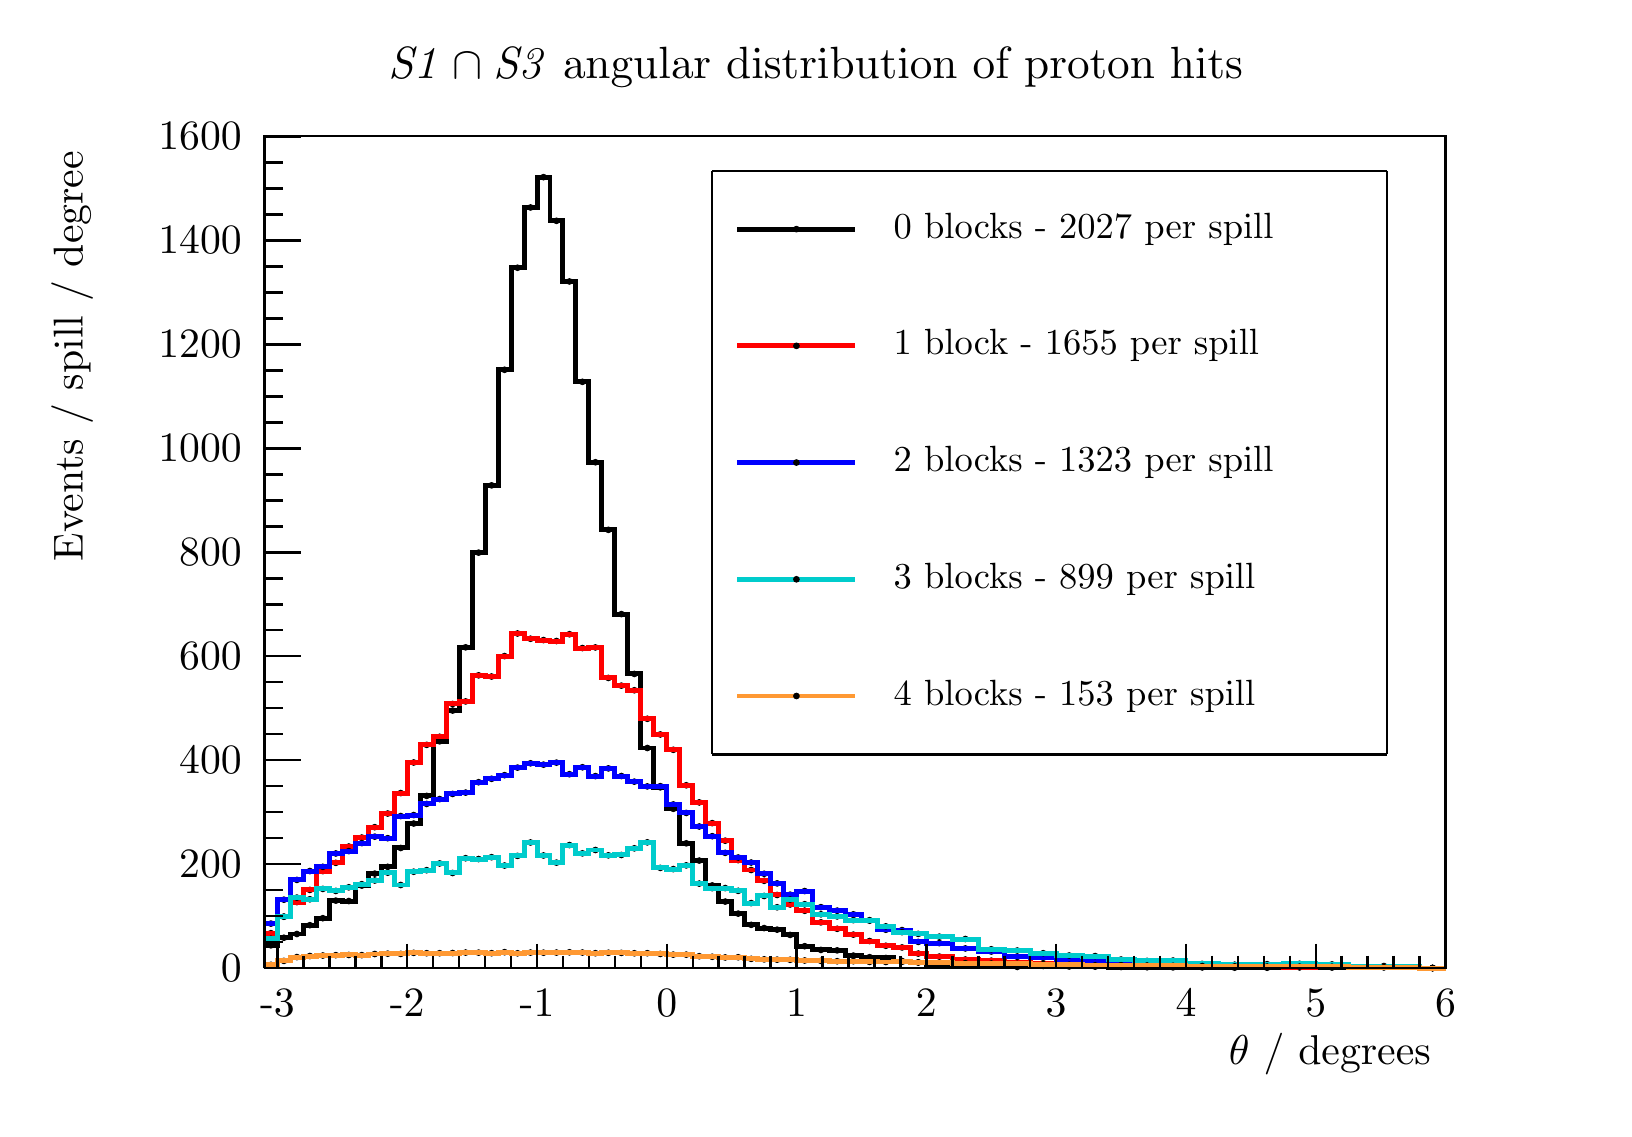
\begin{tikzpicture}
\pgfdeclareplotmark{cross} {
\pgfpathmoveto{\pgfpoint{-0.3\pgfplotmarksize}{\pgfplotmarksize}}
\pgfpathlineto{\pgfpoint{+0.3\pgfplotmarksize}{\pgfplotmarksize}}
\pgfpathlineto{\pgfpoint{+0.3\pgfplotmarksize}{0.3\pgfplotmarksize}}
\pgfpathlineto{\pgfpoint{+1\pgfplotmarksize}{0.3\pgfplotmarksize}}
\pgfpathlineto{\pgfpoint{+1\pgfplotmarksize}{-0.3\pgfplotmarksize}}
\pgfpathlineto{\pgfpoint{+0.3\pgfplotmarksize}{-0.3\pgfplotmarksize}}
\pgfpathlineto{\pgfpoint{+0.3\pgfplotmarksize}{-1.\pgfplotmarksize}}
\pgfpathlineto{\pgfpoint{-0.3\pgfplotmarksize}{-1.\pgfplotmarksize}}
\pgfpathlineto{\pgfpoint{-0.3\pgfplotmarksize}{-0.3\pgfplotmarksize}}
\pgfpathlineto{\pgfpoint{-1.\pgfplotmarksize}{-0.3\pgfplotmarksize}}
\pgfpathlineto{\pgfpoint{-1.\pgfplotmarksize}{0.3\pgfplotmarksize}}
\pgfpathlineto{\pgfpoint{-0.3\pgfplotmarksize}{0.3\pgfplotmarksize}}
\pgfpathclose
\pgfusepathqstroke
}
\pgfdeclareplotmark{cross*} {
\pgfpathmoveto{\pgfpoint{-0.3\pgfplotmarksize}{\pgfplotmarksize}}
\pgfpathlineto{\pgfpoint{+0.3\pgfplotmarksize}{\pgfplotmarksize}}
\pgfpathlineto{\pgfpoint{+0.3\pgfplotmarksize}{0.3\pgfplotmarksize}}
\pgfpathlineto{\pgfpoint{+1\pgfplotmarksize}{0.3\pgfplotmarksize}}
\pgfpathlineto{\pgfpoint{+1\pgfplotmarksize}{-0.3\pgfplotmarksize}}
\pgfpathlineto{\pgfpoint{+0.3\pgfplotmarksize}{-0.3\pgfplotmarksize}}
\pgfpathlineto{\pgfpoint{+0.3\pgfplotmarksize}{-1.\pgfplotmarksize}}
\pgfpathlineto{\pgfpoint{-0.3\pgfplotmarksize}{-1.\pgfplotmarksize}}
\pgfpathlineto{\pgfpoint{-0.3\pgfplotmarksize}{-0.3\pgfplotmarksize}}
\pgfpathlineto{\pgfpoint{-1.\pgfplotmarksize}{-0.3\pgfplotmarksize}}
\pgfpathlineto{\pgfpoint{-1.\pgfplotmarksize}{0.3\pgfplotmarksize}}
\pgfpathlineto{\pgfpoint{-0.3\pgfplotmarksize}{0.3\pgfplotmarksize}}
\pgfpathclose
\pgfusepathqfillstroke
}
\pgfdeclareplotmark{newstar} {
\pgfpathmoveto{\pgfqpoint{0pt}{\pgfplotmarksize}}
\pgfpathlineto{\pgfqpointpolar{44}{0.5\pgfplotmarksize}}
\pgfpathlineto{\pgfqpointpolar{18}{\pgfplotmarksize}}
\pgfpathlineto{\pgfqpointpolar{-20}{0.5\pgfplotmarksize}}
\pgfpathlineto{\pgfqpointpolar{-54}{\pgfplotmarksize}}
\pgfpathlineto{\pgfqpointpolar{-90}{0.5\pgfplotmarksize}}
\pgfpathlineto{\pgfqpointpolar{234}{\pgfplotmarksize}}
\pgfpathlineto{\pgfqpointpolar{198}{0.5\pgfplotmarksize}}
\pgfpathlineto{\pgfqpointpolar{162}{\pgfplotmarksize}}
\pgfpathlineto{\pgfqpointpolar{134}{0.5\pgfplotmarksize}}
\pgfpathclose
\pgfusepathqstroke
}
\pgfdeclareplotmark{newstar*} {
\pgfpathmoveto{\pgfqpoint{0pt}{\pgfplotmarksize}}
\pgfpathlineto{\pgfqpointpolar{44}{0.5\pgfplotmarksize}}
\pgfpathlineto{\pgfqpointpolar{18}{\pgfplotmarksize}}
\pgfpathlineto{\pgfqpointpolar{-20}{0.5\pgfplotmarksize}}
\pgfpathlineto{\pgfqpointpolar{-54}{\pgfplotmarksize}}
\pgfpathlineto{\pgfqpointpolar{-90}{0.5\pgfplotmarksize}}
\pgfpathlineto{\pgfqpointpolar{234}{\pgfplotmarksize}}
\pgfpathlineto{\pgfqpointpolar{198}{0.5\pgfplotmarksize}}
\pgfpathlineto{\pgfqpointpolar{162}{\pgfplotmarksize}}
\pgfpathlineto{\pgfqpointpolar{134}{0.5\pgfplotmarksize}}
\pgfpathclose
\pgfusepathqfillstroke
}
\definecolor{c}{rgb}{1,1,1};
\draw [color=c, fill=c] (0,0) rectangle (20,13.7199);
\draw [color=c, fill=c] (3,1.78359) rectangle (18,12.3479);
\definecolor{c}{rgb}{0,0,0};
\draw [c,line width=0.9] (3,1.78359) -- (3,12.3479) -- (18,12.3479) -- (18,1.78359) -- (3,1.78359);
\definecolor{c}{rgb}{1,1,1};
\draw [color=c, fill=c] (3,1.78359) rectangle (18,12.3479);
\definecolor{c}{rgb}{0,0,0};
\draw [c,line width=0.9] (3,1.78359) -- (3,12.3479) -- (18,12.3479) -- (18,1.78359) -- (3,1.78359);
\definecolor{c}{rgb}{0,0,0.6};
\draw [c,line width=0.9] (3,1.78359) -- (3.16484,1.78359) -- (3.16484,1.78359) -- (3.32967,1.78359) -- (3.32967,1.78359) -- (3.49451,1.78359) -- (3.49451,1.78359) -- (3.65934,1.78359) -- (3.65934,1.78359) -- (3.82418,1.78359) -- (3.82418,1.78359) --
 (3.98901,1.78359) -- (3.98901,1.78359) -- (4.15385,1.78359) -- (4.15385,1.78359) -- (4.31868,1.78359) -- (4.31868,1.78359) -- (4.48352,1.78359) -- (4.48352,1.78359) -- (4.64835,1.78359) -- (4.64835,1.78359) -- (4.81319,1.78359) -- (4.81319,1.78359)
 -- (4.97802,1.78359) -- (4.97802,1.78359) -- (5.14286,1.78359) -- (5.14286,1.78359) -- (5.30769,1.78359) -- (5.30769,1.78359) -- (5.47253,1.78359) -- (5.47253,1.78359) -- (5.63736,1.78359) -- (5.63736,1.78359) -- (5.8022,1.78359) -- (5.8022,1.78359)
 -- (5.96703,1.78359) -- (5.96703,1.78359) -- (6.13187,1.78359) -- (6.13187,1.78359) -- (6.2967,1.78359) -- (6.2967,1.78359) -- (6.46154,1.78359) -- (6.46154,1.78359) -- (6.62637,1.78359) -- (6.62637,1.78359) -- (6.79121,1.78359) -- (6.79121,1.78359)
 -- (6.95604,1.78359) -- (6.95604,1.78359) -- (7.12088,1.78359) -- (7.12088,1.78359) -- (7.28571,1.78359) -- (7.28571,1.78359) -- (7.45055,1.78359) -- (7.45055,1.78359) -- (7.61538,1.78359) -- (7.61538,1.78359) -- (7.78022,1.78359) --
 (7.78022,1.78359) -- (7.94506,1.78359) -- (7.94506,1.78359) -- (8.10989,1.78359) -- (8.10989,1.78359) -- (8.27472,1.78359) -- (8.27472,1.78359) -- (8.43956,1.78359) -- (8.43956,1.78359) -- (8.6044,1.78359) -- (8.6044,1.78359) -- (8.76923,1.78359) --
 (8.76923,1.78359) -- (8.93407,1.78359) -- (8.93407,1.78359) -- (9.0989,1.78359) -- (9.0989,1.78359) -- (9.26374,1.78359) -- (9.26374,1.78359) -- (9.42857,1.78359) -- (9.42857,1.78359) -- (9.59341,1.78359) -- (9.59341,1.78359) -- (9.75824,1.78359) --
 (9.75824,1.78359) -- (9.96429,1.78359) -- (9.96429,1.78359) -- (10.1703,1.78359) -- (10.1703,1.78359) -- (10.3764,1.78359) -- (10.3764,1.78359) -- (10.5824,1.78359) -- (10.5824,1.78359) -- (10.7885,1.78359) -- (10.7885,1.78359) -- (10.9945,1.78359)
 -- (10.9945,1.78359) -- (11.2005,1.78359) -- (11.2005,1.78359) -- (11.4066,1.78359) -- (11.4066,1.78359) -- (11.7363,1.78359) -- (11.7363,1.78359) -- (12.0659,1.78359) -- (12.0659,1.78359) -- (12.3956,1.78359) -- (12.3956,1.78359) --
 (12.7253,1.78359) -- (12.7253,1.78359) -- (13.0549,1.78359) -- (13.0549,1.78359) -- (13.3846,1.78359) -- (13.3846,1.78359) -- (13.7143,1.78359) -- (13.7143,1.78359) -- (14.044,1.78359) -- (14.044,1.78359) -- (14.3736,1.78359) -- (14.3736,1.78359) --
 (14.7033,1.78359) -- (14.7033,1.78359) -- (15.1154,1.78359) -- (15.1154,1.78359) -- (15.5275,1.78359) -- (15.5275,1.78359) -- (15.9396,1.78359) -- (15.9396,1.78359) -- (16.3516,1.78359) -- (16.3516,1.78359) -- (16.7637,1.78359) -- (16.7637,1.78359)
 -- (17.6703,1.78359) -- (17.6703,1.78359) -- (18,1.78359);
\definecolor{c}{rgb}{0,0,0};
\draw [c,line width=0.9] (3,1.78359) -- (18,1.78359);
\draw [c,line width=0.9] (3.16484,2.09229) -- (3.16484,1.78359);
\draw [c,line width=0.9] (3.49451,1.93794) -- (3.49451,1.78359);
\draw [c,line width=0.9] (3.82418,1.93794) -- (3.82418,1.78359);
\draw [c,line width=0.9] (4.15385,1.93794) -- (4.15385,1.78359);
\draw [c,line width=0.9] (4.48352,1.93794) -- (4.48352,1.78359);
\draw [c,line width=0.9] (4.81319,2.09229) -- (4.81319,1.78359);
\draw [c,line width=0.9] (5.14286,1.93794) -- (5.14286,1.78359);
\draw [c,line width=0.9] (5.47253,1.93794) -- (5.47253,1.78359);
\draw [c,line width=0.9] (5.8022,1.93794) -- (5.8022,1.78359);
\draw [c,line width=0.9] (6.13187,1.93794) -- (6.13187,1.78359);
\draw [c,line width=0.9] (6.46154,2.09229) -- (6.46154,1.78359);
\draw [c,line width=0.9] (6.79121,1.93794) -- (6.79121,1.78359);
\draw [c,line width=0.9] (7.12088,1.93794) -- (7.12088,1.78359);
\draw [c,line width=0.9] (7.45055,1.93794) -- (7.45055,1.78359);
\draw [c,line width=0.9] (7.78022,1.93794) -- (7.78022,1.78359);
\draw [c,line width=0.9] (8.10989,2.09229) -- (8.10989,1.78359);
\draw [c,line width=0.9] (8.43956,1.93794) -- (8.43956,1.78359);
\draw [c,line width=0.9] (8.76923,1.93794) -- (8.76923,1.78359);
\draw [c,line width=0.9] (9.0989,1.93794) -- (9.0989,1.78359);
\draw [c,line width=0.9] (9.42857,1.93794) -- (9.42857,1.78359);
\draw [c,line width=0.9] (9.75824,2.09229) -- (9.75824,1.78359);
\draw [c,line width=0.9] (10.0879,1.93794) -- (10.0879,1.78359);
\draw [c,line width=0.9] (10.4176,1.93794) -- (10.4176,1.78359);
\draw [c,line width=0.9] (10.7473,1.93794) -- (10.7473,1.78359);
\draw [c,line width=0.9] (11.0769,1.93794) -- (11.0769,1.78359);
\draw [c,line width=0.9] (11.4066,2.09229) -- (11.4066,1.78359);
\draw [c,line width=0.9] (11.7363,1.93794) -- (11.7363,1.78359);
\draw [c,line width=0.9] (12.0659,1.93794) -- (12.0659,1.78359);
\draw [c,line width=0.9] (12.3956,1.93794) -- (12.3956,1.78359);
\draw [c,line width=0.9] (12.7253,1.93794) -- (12.7253,1.78359);
\draw [c,line width=0.9] (13.0549,2.09229) -- (13.0549,1.78359);
\draw [c,line width=0.9] (13.3846,1.93794) -- (13.3846,1.78359);
\draw [c,line width=0.9] (13.7143,1.93794) -- (13.7143,1.78359);
\draw [c,line width=0.9] (14.044,1.93794) -- (14.044,1.78359);
\draw [c,line width=0.9] (14.3736,1.93794) -- (14.3736,1.78359);
\draw [c,line width=0.9] (14.7033,2.09229) -- (14.7033,1.78359);
\draw [c,line width=0.9] (15.033,1.93794) -- (15.033,1.78359);
\draw [c,line width=0.9] (15.3626,1.93794) -- (15.3626,1.78359);
\draw [c,line width=0.9] (15.6923,1.93794) -- (15.6923,1.78359);
\draw [c,line width=0.9] (16.022,1.93794) -- (16.022,1.78359);
\draw [c,line width=0.9] (16.3516,2.09229) -- (16.3516,1.78359);
\draw [c,line width=0.9] (16.6813,1.93794) -- (16.6813,1.78359);
\draw [c,line width=0.9] (17.011,1.93794) -- (17.011,1.78359);
\draw [c,line width=0.9] (17.3407,1.93794) -- (17.3407,1.78359);
\draw [c,line width=0.9] (17.6703,1.93794) -- (17.6703,1.78359);
\draw [c,line width=0.9] (18,2.09229) -- (18,1.78359);
\draw [c,line width=0.9] (3.16484,2.09229) -- (3.16484,1.78359);
\draw [anchor=base] (3.16484,1.1662) node[scale=1.50787, color=c, rotate=0]{-3};
\draw [anchor=base] (4.81319,1.1662) node[scale=1.50787, color=c, rotate=0]{-2};
\draw [anchor=base] (6.46154,1.1662) node[scale=1.50787, color=c, rotate=0]{-1};
\draw [anchor=base] (8.10989,1.1662) node[scale=1.50787, color=c, rotate=0]{0};
\draw [anchor=base] (9.75824,1.1662) node[scale=1.50787, color=c, rotate=0]{1};
\draw [anchor=base] (11.4066,1.1662) node[scale=1.50787, color=c, rotate=0]{2};
\draw [anchor=base] (13.0549,1.1662) node[scale=1.50787, color=c, rotate=0]{3};
\draw [anchor=base] (14.7033,1.1662) node[scale=1.50787, color=c, rotate=0]{4};
\draw [anchor=base] (16.3516,1.1662) node[scale=1.50787, color=c, rotate=0]{5};
\draw [anchor=base] (18,1.1662) node[scale=1.50787, color=c, rotate=0]{6};
\draw [anchor= east] (18,0.685997) node[scale=1.50787, color=c, rotate=0]{$\theta$ / degrees};
\draw [c,line width=0.9] (3,1.78359) -- (3,12.3479);
\draw [c,line width=0.9] (3.462,1.78359) -- (3,1.78359);
\draw [c,line width=0.9] (3.231,2.11364) -- (3,2.11364);
\draw [c,line width=0.9] (3.231,2.44368) -- (3,2.44368);
\draw [c,line width=0.9] (3.231,2.77373) -- (3,2.77373);
\draw [c,line width=0.9] (3.462,3.10378) -- (3,3.10378);
\draw [c,line width=0.9] (3.231,3.43382) -- (3,3.43382);
\draw [c,line width=0.9] (3.231,3.76387) -- (3,3.76387);
\draw [c,line width=0.9] (3.231,4.09391) -- (3,4.09391);
\draw [c,line width=0.9] (3.462,4.42396) -- (3,4.42396);
\draw [c,line width=0.9] (3.231,4.75401) -- (3,4.75401);
\draw [c,line width=0.9] (3.231,5.08405) -- (3,5.08405);
\draw [c,line width=0.9] (3.231,5.4141) -- (3,5.4141);
\draw [c,line width=0.9] (3.462,5.74414) -- (3,5.74414);
\draw [c,line width=0.9] (3.231,6.07419) -- (3,6.07419);
\draw [c,line width=0.9] (3.231,6.40424) -- (3,6.40424);
\draw [c,line width=0.9] (3.231,6.73428) -- (3,6.73428);
\draw [c,line width=0.9] (3.462,7.06433) -- (3,7.06433);
\draw [c,line width=0.9] (3.231,7.39437) -- (3,7.39437);
\draw [c,line width=0.9] (3.231,7.72442) -- (3,7.72442);
\draw [c,line width=0.9] (3.231,8.05447) -- (3,8.05447);
\draw [c,line width=0.9] (3.462,8.38451) -- (3,8.38451);
\draw [c,line width=0.9] (3.231,8.71456) -- (3,8.71456);
\draw [c,line width=0.9] (3.231,9.04461) -- (3,9.04461);
\draw [c,line width=0.9] (3.231,9.37465) -- (3,9.37465);
\draw [c,line width=0.9] (3.462,9.7047) -- (3,9.7047);
\draw [c,line width=0.9] (3.231,10.0347) -- (3,10.0347);
\draw [c,line width=0.9] (3.231,10.3648) -- (3,10.3648);
\draw [c,line width=0.9] (3.231,10.6948) -- (3,10.6948);
\draw [c,line width=0.9] (3.462,11.0249) -- (3,11.0249);
\draw [c,line width=0.9] (3.231,11.3549) -- (3,11.3549);
\draw [c,line width=0.9] (3.231,11.685) -- (3,11.685);
\draw [c,line width=0.9] (3.231,12.015) -- (3,12.015);
\draw [c,line width=0.9] (3.462,12.3451) -- (3,12.3451);
\draw [c,line width=0.9] (3.462,12.3451) -- (3,12.3451);
\draw [anchor= east] (2.9,1.78359) node[scale=1.50787, color=c, rotate=0]{0};
\draw [anchor= east] (2.9,3.10378) node[scale=1.50787, color=c, rotate=0]{200};
\draw [anchor= east] (2.9,4.42396) node[scale=1.50787, color=c, rotate=0]{400};
\draw [anchor= east] (2.9,5.74414) node[scale=1.50787, color=c, rotate=0]{600};
\draw [anchor= east] (2.9,7.06433) node[scale=1.50787, color=c, rotate=0]{800};
\draw [anchor= east] (2.9,8.38451) node[scale=1.50787, color=c, rotate=0]{1000};
\draw [anchor= east] (2.9,9.7047) node[scale=1.50787, color=c, rotate=0]{1200};
\draw [anchor= east] (2.9,11.0249) node[scale=1.50787, color=c, rotate=0]{1400};
\draw [anchor= east] (2.9,12.3451) node[scale=1.50787, color=c, rotate=0]{1600};
\draw [anchor= east] (0.557284,12.3479) node[scale=1.50787, color=c, rotate=90]{ Events / spill / degree};
\draw [c,line width=1.8] (3.08242,2.06958) -- (3.08242,2.07236);
\draw [c,line width=1.8] (3.08242,2.07236) -- (3.08242,2.07514);
\foreach \P in {(3.08242,2.07236)}{\draw[mark options={color=c,fill=c},mark size=2.402402pt,mark=*,mark size=1pt] plot coordinates {\P};}
\draw [c,line width=1.8] (3.24725,2.16558) -- (3.24725,2.16876);
\draw [c,line width=1.8] (3.24725,2.16876) -- (3.24725,2.17194);
\foreach \P in {(3.24725,2.16876)}{\draw[mark options={color=c,fill=c},mark size=2.402402pt,mark=*,mark size=1pt] plot coordinates {\P};}
\draw [c,line width=1.8] (3.41209,2.21319) -- (3.41209,2.21656);
\draw [c,line width=1.8] (3.41209,2.21656) -- (3.41209,2.21994);
\foreach \P in {(3.41209,2.21656)}{\draw[mark options={color=c,fill=c},mark size=2.402402pt,mark=*,mark size=1pt] plot coordinates {\P};}
\draw [c,line width=1.8] (3.57692,2.32486) -- (3.57692,2.32867);
\draw [c,line width=1.8] (3.57692,2.32867) -- (3.57692,2.33248);
\foreach \P in {(3.57692,2.32867)}{\draw[mark options={color=c,fill=c},mark size=2.402402pt,mark=*,mark size=1pt] plot coordinates {\P};}
\draw [c,line width=1.8] (3.74176,2.41324) -- (3.74176,2.41737);
\draw [c,line width=1.8] (3.74176,2.41737) -- (3.74176,2.42149);
\foreach \P in {(3.74176,2.41737)}{\draw[mark options={color=c,fill=c},mark size=2.402402pt,mark=*,mark size=1pt] plot coordinates {\P};}
\draw [c,line width=1.8] (3.90659,2.63567) -- (3.90659,2.64043);
\draw [c,line width=1.8] (3.90659,2.64043) -- (3.90659,2.6452);
\foreach \P in {(3.90659,2.64043)}{\draw[mark options={color=c,fill=c},mark size=2.402402pt,mark=*,mark size=1pt] plot coordinates {\P};}
\draw [c,line width=1.8] (4.07143,2.63056) -- (4.07143,2.63533);
\draw [c,line width=1.8] (4.07143,2.63533) -- (4.07143,2.6401);
\foreach \P in {(4.07143,2.63533)}{\draw[mark options={color=c,fill=c},mark size=2.402402pt,mark=*,mark size=1pt] plot coordinates {\P};}
\draw [c,line width=1.8] (4.23626,2.82605) -- (4.23626,2.83135);
\draw [c,line width=1.8] (4.23626,2.83135) -- (4.23626,2.83664);
\foreach \P in {(4.23626,2.83135)}{\draw[mark options={color=c,fill=c},mark size=2.402402pt,mark=*,mark size=1pt] plot coordinates {\P};}
\draw [c,line width=1.8] (4.4011,2.97748) -- (4.4011,2.98313);
\draw [c,line width=1.8] (4.4011,2.98313) -- (4.4011,2.98878);
\foreach \P in {(4.4011,2.98313)}{\draw[mark options={color=c,fill=c},mark size=2.402402pt,mark=*,mark size=1pt] plot coordinates {\P};}
\draw [c,line width=1.8] (4.56593,3.06354) -- (4.56593,3.0694);
\draw [c,line width=1.8] (4.56593,3.0694) -- (4.56593,3.07526);
\foreach \P in {(4.56593,3.0694)}{\draw[mark options={color=c,fill=c},mark size=2.402402pt,mark=*,mark size=1pt] plot coordinates {\P};}
\draw [c,line width=1.8] (4.73077,3.30247) -- (4.73077,3.30886);
\draw [c,line width=1.8] (4.73077,3.30886) -- (4.73077,3.31524);
\foreach \P in {(4.73077,3.30886)}{\draw[mark options={color=c,fill=c},mark size=2.402402pt,mark=*,mark size=1pt] plot coordinates {\P};}
\draw [c,line width=1.8] (4.8956,3.61245) -- (4.8956,3.61947);
\draw [c,line width=1.8] (4.8956,3.61947) -- (4.8956,3.62648);
\foreach \P in {(4.8956,3.61947)}{\draw[mark options={color=c,fill=c},mark size=2.402402pt,mark=*,mark size=1pt] plot coordinates {\P};}
\draw [c,line width=1.8] (5.06044,3.96283) -- (5.06044,3.97048);
\draw [c,line width=1.8] (5.06044,3.97048) -- (5.06044,3.97814);
\foreach \P in {(5.06044,3.97048)}{\draw[mark options={color=c,fill=c},mark size=2.402402pt,mark=*,mark size=1pt] plot coordinates {\P};}
\draw [c,line width=1.8] (5.22528,4.65515) -- (5.22528,4.66389);
\draw [c,line width=1.8] (5.22528,4.66389) -- (5.22528,4.67263);
\foreach \P in {(5.22528,4.66389)}{\draw[mark options={color=c,fill=c},mark size=2.402402pt,mark=*,mark size=1pt] plot coordinates {\P};}
\draw [c,line width=1.8] (5.39011,5.04466) -- (5.39011,5.054);
\draw [c,line width=1.8] (5.39011,5.054) -- (5.39011,5.06334);
\foreach \P in {(5.39011,5.054)}{\draw[mark options={color=c,fill=c},mark size=2.402402pt,mark=*,mark size=1pt] plot coordinates {\P};}
\draw [c,line width=1.8] (5.55494,5.84694) -- (5.55494,5.85736);
\draw [c,line width=1.8] (5.55494,5.85736) -- (5.55494,5.86779);
\foreach \P in {(5.55494,5.85736)}{\draw[mark options={color=c,fill=c},mark size=2.402402pt,mark=*,mark size=1pt] plot coordinates {\P};}
\draw [c,line width=1.8] (5.71978,7.04787) -- (5.71978,7.05971);
\draw [c,line width=1.8] (5.71978,7.05971) -- (5.71978,7.07155);
\foreach \P in {(5.71978,7.05971)}{\draw[mark options={color=c,fill=c},mark size=2.402402pt,mark=*,mark size=1pt] plot coordinates {\P};}
\draw [c,line width=1.8] (5.88462,7.90131) -- (5.88462,7.9141);
\draw [c,line width=1.8] (5.88462,7.9141) -- (5.88462,7.9269);
\foreach \P in {(5.88462,7.9141)}{\draw[mark options={color=c,fill=c},mark size=2.402402pt,mark=*,mark size=1pt] plot coordinates {\P};}
\draw [c,line width=1.8] (6.04945,9.36776) -- (6.04945,9.382);
\draw [c,line width=1.8] (6.04945,9.382) -- (6.04945,9.39624);
\foreach \P in {(6.04945,9.382)}{\draw[mark options={color=c,fill=c},mark size=2.402402pt,mark=*,mark size=1pt] plot coordinates {\P};}
\draw [c,line width=1.8] (6.21429,10.6624) -- (6.21429,10.6778);
\draw [c,line width=1.8] (6.21429,10.6778) -- (6.21429,10.6932);
\foreach \P in {(6.21429,10.6778)}{\draw[mark options={color=c,fill=c},mark size=2.402402pt,mark=*,mark size=1pt] plot coordinates {\P};}
\draw [c,line width=1.8] (6.37912,11.4275) -- (6.37912,11.4435);
\draw [c,line width=1.8] (6.37912,11.4435) -- (6.37912,11.4596);
\foreach \P in {(6.37912,11.4435)}{\draw[mark options={color=c,fill=c},mark size=2.402402pt,mark=*,mark size=1pt] plot coordinates {\P};}
\draw [c,line width=1.8] (6.54396,11.8121) -- (6.54396,11.8285);
\draw [c,line width=1.8] (6.54396,11.8285) -- (6.54396,11.8449);
\foreach \P in {(6.54396,11.8285)}{\draw[mark options={color=c,fill=c},mark size=2.402402pt,mark=*,mark size=1pt] plot coordinates {\P};}
\draw [c,line width=1.8] (6.70879,11.2579) -- (6.70879,11.2738);
\draw [c,line width=1.8] (6.70879,11.2738) -- (6.70879,11.2897);
\foreach \P in {(6.70879,11.2738)}{\draw[mark options={color=c,fill=c},mark size=2.402402pt,mark=*,mark size=1pt] plot coordinates {\P};}
\draw [c,line width=1.8] (6.87363,10.4885) -- (6.87363,10.5038);
\draw [c,line width=1.8] (6.87363,10.5038) -- (6.87363,10.5191);
\foreach \P in {(6.87363,10.5038)}{\draw[mark options={color=c,fill=c},mark size=2.402402pt,mark=*,mark size=1pt] plot coordinates {\P};}
\draw [c,line width=1.8] (7.03846,9.21489) -- (7.03846,9.22896);
\draw [c,line width=1.8] (7.03846,9.22896) -- (7.03846,9.24303);
\foreach \P in {(7.03846,9.22896)}{\draw[mark options={color=c,fill=c},mark size=2.402402pt,mark=*,mark size=1pt] plot coordinates {\P};}
\draw [c,line width=1.8] (7.2033,8.19444) -- (7.2033,8.20751);
\draw [c,line width=1.8] (7.2033,8.20751) -- (7.2033,8.22059);
\foreach \P in {(7.2033,8.20751)}{\draw[mark options={color=c,fill=c},mark size=2.402402pt,mark=*,mark size=1pt] plot coordinates {\P};}
\draw [c,line width=1.8] (7.36813,7.33704) -- (7.36813,7.34919);
\draw [c,line width=1.8] (7.36813,7.34919) -- (7.36813,7.36134);
\foreach \P in {(7.36813,7.34919)}{\draw[mark options={color=c,fill=c},mark size=2.402402pt,mark=*,mark size=1pt] plot coordinates {\P};}
\draw [c,line width=1.8] (7.53297,6.26824) -- (7.53297,6.2792);
\draw [c,line width=1.8] (7.53297,6.2792) -- (7.53297,6.29017);
\foreach \P in {(7.53297,6.2792)}{\draw[mark options={color=c,fill=c},mark size=2.402402pt,mark=*,mark size=1pt] plot coordinates {\P};}
\draw [c,line width=1.8] (7.6978,5.50934) -- (7.6978,5.51929);
\draw [c,line width=1.8] (7.6978,5.51929) -- (7.6978,5.52924);
\foreach \P in {(7.6978,5.51929)}{\draw[mark options={color=c,fill=c},mark size=2.402402pt,mark=*,mark size=1pt] plot coordinates {\P};}
\draw [c,line width=1.8] (7.86264,4.57005) -- (7.86264,4.57867);
\draw [c,line width=1.8] (7.86264,4.57867) -- (7.86264,4.58729);
\foreach \P in {(7.86264,4.57867)}{\draw[mark options={color=c,fill=c},mark size=2.402402pt,mark=*,mark size=1pt] plot coordinates {\P};}
\draw [c,line width=1.8] (8.02747,4.07146) -- (8.02747,4.07926);
\draw [c,line width=1.8] (8.02747,4.07926) -- (8.02747,4.08705);
\foreach \P in {(8.02747,4.07926)}{\draw[mark options={color=c,fill=c},mark size=2.402402pt,mark=*,mark size=1pt] plot coordinates {\P};}
\draw [c,line width=1.8] (8.19231,3.79913) -- (8.19231,3.80645);
\draw [c,line width=1.8] (8.19231,3.80645) -- (8.19231,3.81378);
\foreach \P in {(8.19231,3.80645)}{\draw[mark options={color=c,fill=c},mark size=2.402402pt,mark=*,mark size=1pt] plot coordinates {\P};}
\draw [c,line width=1.8] (8.35714,3.36179) -- (8.35714,3.36828);
\draw [c,line width=1.8] (8.35714,3.36828) -- (8.35714,3.37476);
\foreach \P in {(8.35714,3.36828)}{\draw[mark options={color=c,fill=c},mark size=2.402402pt,mark=*,mark size=1pt] plot coordinates {\P};}
\draw [c,line width=1.8] (8.52198,3.14311) -- (8.52198,3.14916);
\draw [c,line width=1.8] (8.52198,3.14916) -- (8.52198,3.1552);
\foreach \P in {(8.52198,3.14916)}{\draw[mark options={color=c,fill=c},mark size=2.402402pt,mark=*,mark size=1pt] plot coordinates {\P};}
\draw [c,line width=1.8] (8.68681,2.82799) -- (8.68681,2.83327);
\draw [c,line width=1.8] (8.68681,2.83327) -- (8.68681,2.83854);
\foreach \P in {(8.68681,2.83327)}{\draw[mark options={color=c,fill=c},mark size=2.402402pt,mark=*,mark size=1pt] plot coordinates {\P};}
\draw [c,line width=1.8] (8.85165,2.62351) -- (8.85165,2.62825);
\draw [c,line width=1.8] (8.85165,2.62825) -- (8.85165,2.63299);
\foreach \P in {(8.85165,2.62825)}{\draw[mark options={color=c,fill=c},mark size=2.402402pt,mark=*,mark size=1pt] plot coordinates {\P};}
\draw [c,line width=1.8] (9.01648,2.47099) -- (9.01648,2.47531);
\draw [c,line width=1.8] (9.01648,2.47531) -- (9.01648,2.47962);
\foreach \P in {(9.01648,2.47531)}{\draw[mark options={color=c,fill=c},mark size=2.402402pt,mark=*,mark size=1pt] plot coordinates {\P};}
\draw [c,line width=1.8] (9.18132,2.32873) -- (9.18132,2.33255);
\draw [c,line width=1.8] (9.18132,2.33255) -- (9.18132,2.33637);
\foreach \P in {(9.18132,2.33255)}{\draw[mark options={color=c,fill=c},mark size=2.402402pt,mark=*,mark size=1pt] plot coordinates {\P};}
\draw [c,line width=1.8] (9.34615,2.28812) -- (9.34615,2.29177);
\draw [c,line width=1.8] (9.34615,2.29177) -- (9.34615,2.29543);
\foreach \P in {(9.34615,2.29177)}{\draw[mark options={color=c,fill=c},mark size=2.402402pt,mark=*,mark size=1pt] plot coordinates {\P};}
\draw [c,line width=1.8] (9.51099,2.26803) -- (9.51099,2.27166);
\draw [c,line width=1.8] (9.51099,2.27166) -- (9.51099,2.27529);
\foreach \P in {(9.51099,2.27166)}{\draw[mark options={color=c,fill=c},mark size=2.402402pt,mark=*,mark size=1pt] plot coordinates {\P};}
\draw [c,line width=1.8] (9.67582,2.20151) -- (9.67582,2.20486);
\draw [c,line width=1.8] (9.67582,2.20486) -- (9.67582,2.20821);
\foreach \P in {(9.67582,2.20486)}{\draw[mark options={color=c,fill=c},mark size=2.402402pt,mark=*,mark size=1pt] plot coordinates {\P};}
\draw [c,line width=1.8] (9.86126,2.05878) -- (9.86126,2.06181);
\draw [c,line width=1.8] (9.86126,2.06181) -- (9.86126,2.06484);
\foreach \P in {(9.86126,2.06181)}{\draw[mark options={color=c,fill=c},mark size=2.402402pt,mark=*,mark size=1pt] plot coordinates {\P};}
\draw [c,line width=1.8] (10.0673,2.01154) -- (10.0673,2.01434);
\draw [c,line width=1.8] (10.0673,2.01434) -- (10.0673,2.01713);
\foreach \P in {(10.0673,2.01434)}{\draw[mark options={color=c,fill=c},mark size=2.402402pt,mark=*,mark size=1pt] plot coordinates {\P};}
\draw [c,line width=1.8] (10.2734,2.00588) -- (10.2734,2.00861);
\draw [c,line width=1.8] (10.2734,2.00861) -- (10.2734,2.01134);
\foreach \P in {(10.2734,2.00861)}{\draw[mark options={color=c,fill=c},mark size=2.402402pt,mark=*,mark size=1pt] plot coordinates {\P};}
\draw [c,line width=1.8] (10.4794,1.94002) -- (10.4794,1.94233);
\draw [c,line width=1.8] (10.4794,1.94233) -- (10.4794,1.94463);
\foreach \P in {(10.4794,1.94233)}{\draw[mark options={color=c,fill=c},mark size=2.402402pt,mark=*,mark size=1pt] plot coordinates {\P};}
\draw [c,line width=1.8] (10.6854,1.92022) -- (10.6854,1.92239);
\draw [c,line width=1.8] (10.6854,1.92239) -- (10.6854,1.92455);
\foreach \P in {(10.6854,1.92239)}{\draw[mark options={color=c,fill=c},mark size=2.402402pt,mark=*,mark size=1pt] plot coordinates {\P};}
\draw [c,line width=1.8] (10.8915,1.90989) -- (10.8915,1.91196);
\draw [c,line width=1.8] (10.8915,1.91196) -- (10.8915,1.91402);
\foreach \P in {(10.8915,1.91196)}{\draw[mark options={color=c,fill=c},mark size=2.402402pt,mark=*,mark size=1pt] plot coordinates {\P};}
\draw [c,line width=1.8] (11.0975,1.87185) -- (11.0975,1.87359);
\draw [c,line width=1.8] (11.0975,1.87359) -- (11.0975,1.87533);
\foreach \P in {(11.0975,1.87359)}{\draw[mark options={color=c,fill=c},mark size=2.402402pt,mark=*,mark size=1pt] plot coordinates {\P};}
\draw [c,line width=1.8] (11.3036,1.85511) -- (11.3036,1.85664);
\draw [c,line width=1.8] (11.3036,1.85664) -- (11.3036,1.85816);
\foreach \P in {(11.3036,1.85664)}{\draw[mark options={color=c,fill=c},mark size=2.402402pt,mark=*,mark size=1pt] plot coordinates {\P};}
\draw [c,line width=1.8] (11.5714,1.82366) -- (11.5714,1.82514);
\draw [c,line width=1.8] (11.5714,1.82514) -- (11.5714,1.82662);
\foreach \P in {(11.5714,1.82514)}{\draw[mark options={color=c,fill=c},mark size=2.402402pt,mark=*,mark size=1pt] plot coordinates {\P};}
\draw [c,line width=1.8] (11.9011,1.83059) -- (11.9011,1.83222);
\draw [c,line width=1.8] (11.9011,1.83222) -- (11.9011,1.83385);
\foreach \P in {(11.9011,1.83222)}{\draw[mark options={color=c,fill=c},mark size=2.402402pt,mark=*,mark size=1pt] plot coordinates {\P};}
\draw [c,line width=1.8] (12.2308,1.81449) -- (12.2308,1.81579);
\draw [c,line width=1.8] (12.2308,1.81579) -- (12.2308,1.81709);
\foreach \P in {(12.2308,1.81579)}{\draw[mark options={color=c,fill=c},mark size=2.402402pt,mark=*,mark size=1pt] plot coordinates {\P};}
\draw [c,line width=1.8] (12.5604,1.79787) -- (12.5604,1.79879);
\draw [c,line width=1.8] (12.5604,1.79879) -- (12.5604,1.79971);
\foreach \P in {(12.5604,1.79879)}{\draw[mark options={color=c,fill=c},mark size=2.402402pt,mark=*,mark size=1pt] plot coordinates {\P};}
\draw [c,line width=1.8] (12.8901,1.80983) -- (12.8901,1.81104);
\draw [c,line width=1.8] (12.8901,1.81104) -- (12.8901,1.81224);
\foreach \P in {(12.8901,1.81104)}{\draw[mark options={color=c,fill=c},mark size=2.402402pt,mark=*,mark size=1pt] plot coordinates {\P};}
\draw [c,line width=1.8] (13.2198,1.80291) -- (13.2198,1.80396);
\draw [c,line width=1.8] (13.2198,1.80396) -- (13.2198,1.80502);
\foreach \P in {(13.2198,1.80396)}{\draw[mark options={color=c,fill=c},mark size=2.402402pt,mark=*,mark size=1pt] plot coordinates {\P};}
\draw [c,line width=1.8] (13.5495,1.80101) -- (13.5495,1.80199);
\draw [c,line width=1.8] (13.5495,1.80199) -- (13.5495,1.80298);
\foreach \P in {(13.5495,1.80199)}{\draw[mark options={color=c,fill=c},mark size=2.402402pt,mark=*,mark size=1pt] plot coordinates {\P};}
\draw [c,line width=1.8] (13.8791,1.79634) -- (13.8791,1.7972);
\draw [c,line width=1.8] (13.8791,1.7972) -- (13.8791,1.79807);
\foreach \P in {(13.8791,1.7972)}{\draw[mark options={color=c,fill=c},mark size=2.402402pt,mark=*,mark size=1pt] plot coordinates {\P};}
\draw [c,line width=1.8] (14.2088,1.79354) -- (14.2088,1.7943);
\draw [c,line width=1.8] (14.2088,1.7943) -- (14.2088,1.79506);
\foreach \P in {(14.2088,1.7943)}{\draw[mark options={color=c,fill=c},mark size=2.402402pt,mark=*,mark size=1pt] plot coordinates {\P};}
\draw [c,line width=1.8] (14.5385,1.79198) -- (14.5385,1.79267);
\draw [c,line width=1.8] (14.5385,1.79267) -- (14.5385,1.79336);
\foreach \P in {(14.5385,1.79267)}{\draw[mark options={color=c,fill=c},mark size=2.402402pt,mark=*,mark size=1pt] plot coordinates {\P};}
\draw [c,line width=1.8] (14.9093,1.79118) -- (14.9093,1.79192);
\draw [c,line width=1.8] (14.9093,1.79192) -- (14.9093,1.79265);
\foreach \P in {(14.9093,1.79192)}{\draw[mark options={color=c,fill=c},mark size=2.402402pt,mark=*,mark size=1pt] plot coordinates {\P};}
\draw [c,line width=1.8] (15.3214,1.78811) -- (15.3214,1.78869);
\draw [c,line width=1.8] (15.3214,1.78869) -- (15.3214,1.78926);
\foreach \P in {(15.3214,1.78869)}{\draw[mark options={color=c,fill=c},mark size=2.402402pt,mark=*,mark size=1pt] plot coordinates {\P};}
\draw [c,line width=1.8] (15.7335,1.78719) -- (15.7335,1.7877);
\draw [c,line width=1.8] (15.7335,1.7877) -- (15.7335,1.78822);
\foreach \P in {(15.7335,1.7877)}{\draw[mark options={color=c,fill=c},mark size=2.402402pt,mark=*,mark size=1pt] plot coordinates {\P};}
\draw [c,line width=1.8] (16.1456,1.79238) -- (16.1456,1.79319);
\draw [c,line width=1.8] (16.1456,1.79319) -- (16.1456,1.79399);
\foreach \P in {(16.1456,1.79319)}{\draw[mark options={color=c,fill=c},mark size=2.402402pt,mark=*,mark size=1pt] plot coordinates {\P};}
\draw [c,line width=1.8] (16.5577,1.78968) -- (16.5577,1.79038);
\draw [c,line width=1.8] (16.5577,1.79038) -- (16.5577,1.79107);
\foreach \P in {(16.5577,1.79038)}{\draw[mark options={color=c,fill=c},mark size=2.402402pt,mark=*,mark size=1pt] plot coordinates {\P};}
\draw [c,line width=1.8] (17.217,1.7914) -- (17.217,1.79253);
\draw [c,line width=1.8] (17.217,1.79253) -- (17.217,1.79367);
\foreach \P in {(17.217,1.79253)}{\draw[mark options={color=c,fill=c},mark size=2.402402pt,mark=*,mark size=1pt] plot coordinates {\P};}
\draw [c,line width=1.8] (17.8352,1.7841) -- (17.8352,1.78462);
\draw [c,line width=1.8] (17.8352,1.78462) -- (17.8352,1.78513);
\foreach \P in {(17.8352,1.78462)}{\draw[mark options={color=c,fill=c},mark size=2.402402pt,mark=*,mark size=1pt] plot coordinates {\P};}
\draw [c,line width=1.8] (3,2.07236) -- (3.16484,2.07236) -- (3.16484,2.16876) -- (3.32967,2.16876) -- (3.32967,2.21656) -- (3.49451,2.21656) -- (3.49451,2.32867) -- (3.65934,2.32867) -- (3.65934,2.41737) -- (3.82418,2.41737) -- (3.82418,2.64043) --
 (3.98901,2.64043) -- (3.98901,2.63533) -- (4.15385,2.63533) -- (4.15385,2.83135) -- (4.31868,2.83135) -- (4.31868,2.98313) -- (4.48352,2.98313) -- (4.48352,3.0694) -- (4.64835,3.0694) -- (4.64835,3.30886) -- (4.81319,3.30886) -- (4.81319,3.61947) --
 (4.97802,3.61947) -- (4.97802,3.97048) -- (5.14286,3.97048) -- (5.14286,4.66389) -- (5.30769,4.66389) -- (5.30769,5.054) -- (5.47253,5.054) -- (5.47253,5.85736) -- (5.63736,5.85736) -- (5.63736,7.05971) -- (5.8022,7.05971) -- (5.8022,7.9141) --
 (5.96703,7.9141) -- (5.96703,9.382) -- (6.13187,9.382) -- (6.13187,10.6778) -- (6.2967,10.6778) -- (6.2967,11.4435) -- (6.46154,11.4435) -- (6.46154,11.8285) -- (6.62637,11.8285) -- (6.62637,11.2738) -- (6.79121,11.2738) -- (6.79121,10.5038) --
 (6.95604,10.5038) -- (6.95604,9.22896) -- (7.12088,9.22896) -- (7.12088,8.20751) -- (7.28571,8.20751) -- (7.28571,7.34919) -- (7.45055,7.34919) -- (7.45055,6.2792) -- (7.61538,6.2792) -- (7.61538,5.51929) -- (7.78022,5.51929) -- (7.78022,4.57867) --
 (7.94506,4.57867) -- (7.94506,4.07926) -- (8.10989,4.07926) -- (8.10989,3.80645) -- (8.27472,3.80645) -- (8.27472,3.36828) -- (8.43956,3.36828) -- (8.43956,3.14916) -- (8.6044,3.14916) -- (8.6044,2.83327) -- (8.76923,2.83327) -- (8.76923,2.62825) --
 (8.93407,2.62825) -- (8.93407,2.47531) -- (9.0989,2.47531) -- (9.0989,2.33255) -- (9.26374,2.33255) -- (9.26374,2.29177) -- (9.42857,2.29177) -- (9.42857,2.27166) -- (9.59341,2.27166) -- (9.59341,2.20486) -- (9.75824,2.20486) -- (9.75824,2.06181) --
 (9.96429,2.06181) -- (9.96429,2.01434) -- (10.1703,2.01434) -- (10.1703,2.00861) -- (10.3764,2.00861) -- (10.3764,1.94233) -- (10.5824,1.94233) -- (10.5824,1.92239) -- (10.7885,1.92239) -- (10.7885,1.91196) -- (10.9945,1.91196) -- (10.9945,1.87359)
 -- (11.2005,1.87359) -- (11.2005,1.85664) -- (11.4066,1.85664) -- (11.4066,1.82514) -- (11.7363,1.82514) -- (11.7363,1.83222) -- (12.0659,1.83222) -- (12.0659,1.81579) -- (12.3956,1.81579) -- (12.3956,1.79879) -- (12.7253,1.79879) --
 (12.7253,1.81104) -- (13.0549,1.81104) -- (13.0549,1.80396) -- (13.3846,1.80396) -- (13.3846,1.80199) -- (13.7143,1.80199) -- (13.7143,1.7972) -- (14.044,1.7972) -- (14.044,1.7943) -- (14.3736,1.7943) -- (14.3736,1.79267) -- (14.7033,1.79267) --
 (14.7033,1.79192) -- (15.1154,1.79192) -- (15.1154,1.78869) -- (15.5275,1.78869) -- (15.5275,1.7877) -- (15.9396,1.7877) -- (15.9396,1.79319) -- (16.3516,1.79319) -- (16.3516,1.79038) -- (16.7637,1.79038) -- (16.7637,1.79253) -- (17.6703,1.79253) --
 (17.6703,1.78359) -- (18,1.78359);
\definecolor{c}{rgb}{1,0,0};
\draw [c,line width=1.8] (3.08242,2.22427) -- (3.08242,2.22712);
\draw [c,line width=1.8] (3.08242,2.22712) -- (3.08242,2.22997);
\definecolor{c}{rgb}{0,0,0};
\foreach \P in {(3.08242,2.22712)}{\draw[mark options={color=c,fill=c},mark size=2.402402pt,mark=*,mark size=1pt] plot coordinates {\P};}
\definecolor{c}{rgb}{1,0,0};
\draw [c,line width=1.8] (3.24725,2.43254) -- (3.24725,2.436);
\draw [c,line width=1.8] (3.24725,2.436) -- (3.24725,2.43945);
\definecolor{c}{rgb}{0,0,0};
\foreach \P in {(3.24725,2.436)}{\draw[mark options={color=c,fill=c},mark size=2.402402pt,mark=*,mark size=1pt] plot coordinates {\P};}
\definecolor{c}{rgb}{1,0,0};
\draw [c,line width=1.8] (3.41209,2.61816) -- (3.41209,2.62207);
\draw [c,line width=1.8] (3.41209,2.62207) -- (3.41209,2.62598);
\definecolor{c}{rgb}{0,0,0};
\foreach \P in {(3.41209,2.62207)}{\draw[mark options={color=c,fill=c},mark size=2.402402pt,mark=*,mark size=1pt] plot coordinates {\P};}
\definecolor{c}{rgb}{1,0,0};
\draw [c,line width=1.8] (3.57692,2.77196) -- (3.57692,2.77623);
\draw [c,line width=1.8] (3.57692,2.77623) -- (3.57692,2.7805);
\definecolor{c}{rgb}{0,0,0};
\foreach \P in {(3.57692,2.77623)}{\draw[mark options={color=c,fill=c},mark size=2.402402pt,mark=*,mark size=1pt] plot coordinates {\P};}
\definecolor{c}{rgb}{1,0,0};
\draw [c,line width=1.8] (3.74176,3.01057) -- (3.74176,3.01529);
\draw [c,line width=1.8] (3.74176,3.01529) -- (3.74176,3.02002);
\definecolor{c}{rgb}{0,0,0};
\foreach \P in {(3.74176,3.01529)}{\draw[mark options={color=c,fill=c},mark size=2.402402pt,mark=*,mark size=1pt] plot coordinates {\P};}
\definecolor{c}{rgb}{1,0,0};
\draw [c,line width=1.8] (3.90659,3.11529) -- (3.90659,3.12021);
\draw [c,line width=1.8] (3.90659,3.12021) -- (3.90659,3.12512);
\definecolor{c}{rgb}{0,0,0};
\foreach \P in {(3.90659,3.12021)}{\draw[mark options={color=c,fill=c},mark size=2.402402pt,mark=*,mark size=1pt] plot coordinates {\P};}
\definecolor{c}{rgb}{1,0,0};
\draw [c,line width=1.8] (4.07143,3.32198) -- (4.07143,3.32729);
\draw [c,line width=1.8] (4.07143,3.32729) -- (4.07143,3.33261);
\definecolor{c}{rgb}{0,0,0};
\foreach \P in {(4.07143,3.32729)}{\draw[mark options={color=c,fill=c},mark size=2.402402pt,mark=*,mark size=1pt] plot coordinates {\P};}
\definecolor{c}{rgb}{1,0,0};
\draw [c,line width=1.8] (4.23626,3.43592) -- (4.23626,3.44141);
\draw [c,line width=1.8] (4.23626,3.44141) -- (4.23626,3.44689);
\definecolor{c}{rgb}{0,0,0};
\foreach \P in {(4.23626,3.44141)}{\draw[mark options={color=c,fill=c},mark size=2.402402pt,mark=*,mark size=1pt] plot coordinates {\P};}
\definecolor{c}{rgb}{1,0,0};
\draw [c,line width=1.8] (4.4011,3.56762) -- (4.4011,3.57336);
\draw [c,line width=1.8] (4.4011,3.57336) -- (4.4011,3.5791);
\definecolor{c}{rgb}{0,0,0};
\foreach \P in {(4.4011,3.57336)}{\draw[mark options={color=c,fill=c},mark size=2.402402pt,mark=*,mark size=1pt] plot coordinates {\P};}
\definecolor{c}{rgb}{1,0,0};
\draw [c,line width=1.8] (4.56593,3.74068) -- (4.56593,3.74667);
\draw [c,line width=1.8] (4.56593,3.74667) -- (4.56593,3.75266);
\definecolor{c}{rgb}{0,0,0};
\foreach \P in {(4.56593,3.74667)}{\draw[mark options={color=c,fill=c},mark size=2.402402pt,mark=*,mark size=1pt] plot coordinates {\P};}
\definecolor{c}{rgb}{1,0,0};
\draw [c,line width=1.8] (4.73077,3.99987) -- (4.73077,4.00622);
\draw [c,line width=1.8] (4.73077,4.00622) -- (4.73077,4.01258);
\definecolor{c}{rgb}{0,0,0};
\foreach \P in {(4.73077,4.00622)}{\draw[mark options={color=c,fill=c},mark size=2.402402pt,mark=*,mark size=1pt] plot coordinates {\P};}
\definecolor{c}{rgb}{1,0,0};
\draw [c,line width=1.8] (4.8956,4.38771) -- (4.8956,4.3946);
\draw [c,line width=1.8] (4.8956,4.3946) -- (4.8956,4.40148);
\definecolor{c}{rgb}{0,0,0};
\foreach \P in {(4.8956,4.3946)}{\draw[mark options={color=c,fill=c},mark size=2.402402pt,mark=*,mark size=1pt] plot coordinates {\P};}
\definecolor{c}{rgb}{1,0,0};
\draw [c,line width=1.8] (5.06044,4.61128) -- (5.06044,4.61847);
\draw [c,line width=1.8] (5.06044,4.61847) -- (5.06044,4.62566);
\definecolor{c}{rgb}{0,0,0};
\foreach \P in {(5.06044,4.61847)}{\draw[mark options={color=c,fill=c},mark size=2.402402pt,mark=*,mark size=1pt] plot coordinates {\P};}
\definecolor{c}{rgb}{1,0,0};
\draw [c,line width=1.8] (5.22528,4.71391) -- (5.22528,4.7212);
\draw [c,line width=1.8] (5.22528,4.7212) -- (5.22528,4.72849);
\definecolor{c}{rgb}{0,0,0};
\foreach \P in {(5.22528,4.7212)}{\draw[mark options={color=c,fill=c},mark size=2.402402pt,mark=*,mark size=1pt] plot coordinates {\P};}
\definecolor{c}{rgb}{1,0,0};
\draw [c,line width=1.8] (5.39011,5.12986) -- (5.39011,5.13767);
\draw [c,line width=1.8] (5.39011,5.13767) -- (5.39011,5.14549);
\definecolor{c}{rgb}{0,0,0};
\foreach \P in {(5.39011,5.13767)}{\draw[mark options={color=c,fill=c},mark size=2.402402pt,mark=*,mark size=1pt] plot coordinates {\P};}
\definecolor{c}{rgb}{1,0,0};
\draw [c,line width=1.8] (5.55494,5.1625) -- (5.55494,5.17034);
\draw [c,line width=1.8] (5.55494,5.17034) -- (5.55494,5.17819);
\definecolor{c}{rgb}{0,0,0};
\foreach \P in {(5.55494,5.17034)}{\draw[mark options={color=c,fill=c},mark size=2.402402pt,mark=*,mark size=1pt] plot coordinates {\P};}
\definecolor{c}{rgb}{1,0,0};
\draw [c,line width=1.8] (5.71978,5.49334) -- (5.71978,5.50155);
\draw [c,line width=1.8] (5.71978,5.50155) -- (5.71978,5.50976);
\definecolor{c}{rgb}{0,0,0};
\foreach \P in {(5.71978,5.50155)}{\draw[mark options={color=c,fill=c},mark size=2.402402pt,mark=*,mark size=1pt] plot coordinates {\P};}
\definecolor{c}{rgb}{1,0,0};
\draw [c,line width=1.8] (5.88462,5.47831) -- (5.88462,5.48654);
\draw [c,line width=1.8] (5.88462,5.48654) -- (5.88462,5.49476);
\definecolor{c}{rgb}{0,0,0};
\foreach \P in {(5.88462,5.48654)}{\draw[mark options={color=c,fill=c},mark size=2.402402pt,mark=*,mark size=1pt] plot coordinates {\P};}
\definecolor{c}{rgb}{1,0,0};
\draw [c,line width=1.8] (6.04945,5.73748) -- (6.04945,5.74598);
\draw [c,line width=1.8] (6.04945,5.74598) -- (6.04945,5.75448);
\definecolor{c}{rgb}{0,0,0};
\foreach \P in {(6.04945,5.74598)}{\draw[mark options={color=c,fill=c},mark size=2.402402pt,mark=*,mark size=1pt] plot coordinates {\P};}
\definecolor{c}{rgb}{1,0,0};
\draw [c,line width=1.8] (6.21429,6.0244) -- (6.21429,6.03319);
\draw [c,line width=1.8] (6.21429,6.03319) -- (6.21429,6.04198);
\definecolor{c}{rgb}{0,0,0};
\foreach \P in {(6.21429,6.03319)}{\draw[mark options={color=c,fill=c},mark size=2.402402pt,mark=*,mark size=1pt] plot coordinates {\P};}
\definecolor{c}{rgb}{1,0,0};
\draw [c,line width=1.8] (6.37912,5.9575) -- (6.37912,5.96625);
\draw [c,line width=1.8] (6.37912,5.96625) -- (6.37912,5.97501);
\definecolor{c}{rgb}{0,0,0};
\foreach \P in {(6.37912,5.96625)}{\draw[mark options={color=c,fill=c},mark size=2.402402pt,mark=*,mark size=1pt] plot coordinates {\P};}
\definecolor{c}{rgb}{1,0,0};
\draw [c,line width=1.8] (6.54396,5.9409) -- (6.54396,5.94961);
\draw [c,line width=1.8] (6.54396,5.94961) -- (6.54396,5.95833);
\definecolor{c}{rgb}{0,0,0};
\foreach \P in {(6.54396,5.94961)}{\draw[mark options={color=c,fill=c},mark size=2.402402pt,mark=*,mark size=1pt] plot coordinates {\P};}
\definecolor{c}{rgb}{1,0,0};
\draw [c,line width=1.8] (6.70879,5.92867) -- (6.70879,5.93738);
\draw [c,line width=1.8] (6.70879,5.93738) -- (6.70879,5.94608);
\definecolor{c}{rgb}{0,0,0};
\foreach \P in {(6.70879,5.93738)}{\draw[mark options={color=c,fill=c},mark size=2.402402pt,mark=*,mark size=1pt] plot coordinates {\P};}
\definecolor{c}{rgb}{1,0,0};
\draw [c,line width=1.8] (6.87363,6.01485) -- (6.87363,6.02367);
\draw [c,line width=1.8] (6.87363,6.02367) -- (6.87363,6.03249);
\definecolor{c}{rgb}{0,0,0};
\foreach \P in {(6.87363,6.02367)}{\draw[mark options={color=c,fill=c},mark size=2.402402pt,mark=*,mark size=1pt] plot coordinates {\P};}
\definecolor{c}{rgb}{1,0,0};
\draw [c,line width=1.8] (7.03846,5.83959) -- (7.03846,5.84817);
\draw [c,line width=1.8] (7.03846,5.84817) -- (7.03846,5.85675);
\definecolor{c}{rgb}{0,0,0};
\foreach \P in {(7.03846,5.84817)}{\draw[mark options={color=c,fill=c},mark size=2.402402pt,mark=*,mark size=1pt] plot coordinates {\P};}
\definecolor{c}{rgb}{1,0,0};
\draw [c,line width=1.8] (7.2033,5.84737) -- (7.2033,5.856);
\draw [c,line width=1.8] (7.2033,5.856) -- (7.2033,5.86464);
\definecolor{c}{rgb}{0,0,0};
\foreach \P in {(7.2033,5.856)}{\draw[mark options={color=c,fill=c},mark size=2.402402pt,mark=*,mark size=1pt] plot coordinates {\P};}
\definecolor{c}{rgb}{1,0,0};
\draw [c,line width=1.8] (7.36813,5.46039) -- (7.36813,5.4686);
\draw [c,line width=1.8] (7.36813,5.4686) -- (7.36813,5.4768);
\definecolor{c}{rgb}{0,0,0};
\foreach \P in {(7.36813,5.4686)}{\draw[mark options={color=c,fill=c},mark size=2.402402pt,mark=*,mark size=1pt] plot coordinates {\P};}
\definecolor{c}{rgb}{1,0,0};
\draw [c,line width=1.8] (7.53297,5.36276) -- (7.53297,5.37084);
\draw [c,line width=1.8] (7.53297,5.37084) -- (7.53297,5.37893);
\definecolor{c}{rgb}{0,0,0};
\foreach \P in {(7.53297,5.37084)}{\draw[mark options={color=c,fill=c},mark size=2.402402pt,mark=*,mark size=1pt] plot coordinates {\P};}
\definecolor{c}{rgb}{1,0,0};
\draw [c,line width=1.8] (7.6978,5.30408) -- (7.6978,5.31212);
\draw [c,line width=1.8] (7.6978,5.31212) -- (7.6978,5.32016);
\definecolor{c}{rgb}{0,0,0};
\foreach \P in {(7.6978,5.31212)}{\draw[mark options={color=c,fill=c},mark size=2.402402pt,mark=*,mark size=1pt] plot coordinates {\P};}
\definecolor{c}{rgb}{1,0,0};
\draw [c,line width=1.8] (7.86264,4.94216) -- (7.86264,4.94975);
\draw [c,line width=1.8] (7.86264,4.94975) -- (7.86264,4.95734);
\definecolor{c}{rgb}{0,0,0};
\foreach \P in {(7.86264,4.94975)}{\draw[mark options={color=c,fill=c},mark size=2.402402pt,mark=*,mark size=1pt] plot coordinates {\P};}
\definecolor{c}{rgb}{1,0,0};
\draw [c,line width=1.8] (8.02747,4.74325) -- (8.02747,4.75061);
\draw [c,line width=1.8] (8.02747,4.75061) -- (8.02747,4.75798);
\definecolor{c}{rgb}{0,0,0};
\foreach \P in {(8.02747,4.75061)}{\draw[mark options={color=c,fill=c},mark size=2.402402pt,mark=*,mark size=1pt] plot coordinates {\P};}
\definecolor{c}{rgb}{1,0,0};
\draw [c,line width=1.8] (8.19231,4.54864) -- (8.19231,4.55573);
\draw [c,line width=1.8] (8.19231,4.55573) -- (8.19231,4.56283);
\definecolor{c}{rgb}{0,0,0};
\foreach \P in {(8.19231,4.55573)}{\draw[mark options={color=c,fill=c},mark size=2.402402pt,mark=*,mark size=1pt] plot coordinates {\P};}
\definecolor{c}{rgb}{1,0,0};
\draw [c,line width=1.8] (8.35714,4.09901) -- (8.35714,4.10554);
\draw [c,line width=1.8] (8.35714,4.10554) -- (8.35714,4.11207);
\definecolor{c}{rgb}{0,0,0};
\foreach \P in {(8.35714,4.10554)}{\draw[mark options={color=c,fill=c},mark size=2.402402pt,mark=*,mark size=1pt] plot coordinates {\P};}
\definecolor{c}{rgb}{1,0,0};
\draw [c,line width=1.8] (8.52198,3.88173) -- (8.52198,3.88792);
\draw [c,line width=1.8] (8.52198,3.88792) -- (8.52198,3.89411);
\definecolor{c}{rgb}{0,0,0};
\foreach \P in {(8.52198,3.88792)}{\draw[mark options={color=c,fill=c},mark size=2.402402pt,mark=*,mark size=1pt] plot coordinates {\P};}
\definecolor{c}{rgb}{1,0,0};
\draw [c,line width=1.8] (8.68681,3.61894) -- (8.68681,3.62474);
\draw [c,line width=1.8] (8.68681,3.62474) -- (8.68681,3.63053);
\definecolor{c}{rgb}{0,0,0};
\foreach \P in {(8.68681,3.62474)}{\draw[mark options={color=c,fill=c},mark size=2.402402pt,mark=*,mark size=1pt] plot coordinates {\P};}
\definecolor{c}{rgb}{1,0,0};
\draw [c,line width=1.8] (8.85165,3.39616) -- (8.85165,3.40156);
\draw [c,line width=1.8] (8.85165,3.40156) -- (8.85165,3.40696);
\definecolor{c}{rgb}{0,0,0};
\foreach \P in {(8.85165,3.40156)}{\draw[mark options={color=c,fill=c},mark size=2.402402pt,mark=*,mark size=1pt] plot coordinates {\P};}
\definecolor{c}{rgb}{1,0,0};
\draw [c,line width=1.8] (9.01648,3.14986) -- (9.01648,3.15485);
\draw [c,line width=1.8] (9.01648,3.15485) -- (9.01648,3.15984);
\definecolor{c}{rgb}{0,0,0};
\foreach \P in {(9.01648,3.15485)}{\draw[mark options={color=c,fill=c},mark size=2.402402pt,mark=*,mark size=1pt] plot coordinates {\P};}
\definecolor{c}{rgb}{1,0,0};
\draw [c,line width=1.8] (9.18132,3.02449) -- (9.18132,3.02926);
\draw [c,line width=1.8] (9.18132,3.02926) -- (9.18132,3.03402);
\definecolor{c}{rgb}{0,0,0};
\foreach \P in {(9.18132,3.02926)}{\draw[mark options={color=c,fill=c},mark size=2.402402pt,mark=*,mark size=1pt] plot coordinates {\P};}
\definecolor{c}{rgb}{1,0,0};
\draw [c,line width=1.8] (9.34615,2.88758) -- (9.34615,2.89207);
\draw [c,line width=1.8] (9.34615,2.89207) -- (9.34615,2.89657);
\definecolor{c}{rgb}{0,0,0};
\foreach \P in {(9.34615,2.89207)}{\draw[mark options={color=c,fill=c},mark size=2.402402pt,mark=*,mark size=1pt] plot coordinates {\P};}
\definecolor{c}{rgb}{1,0,0};
\draw [c,line width=1.8] (9.51099,2.70786) -- (9.51099,2.71198);
\draw [c,line width=1.8] (9.51099,2.71198) -- (9.51099,2.7161);
\definecolor{c}{rgb}{0,0,0};
\foreach \P in {(9.51099,2.71198)}{\draw[mark options={color=c,fill=c},mark size=2.402402pt,mark=*,mark size=1pt] plot coordinates {\P};}
\definecolor{c}{rgb}{1,0,0};
\draw [c,line width=1.8] (9.67582,2.58775) -- (9.67582,2.59161);
\draw [c,line width=1.8] (9.67582,2.59161) -- (9.67582,2.59546);
\definecolor{c}{rgb}{0,0,0};
\foreach \P in {(9.67582,2.59161)}{\draw[mark options={color=c,fill=c},mark size=2.402402pt,mark=*,mark size=1pt] plot coordinates {\P};}
\definecolor{c}{rgb}{1,0,0};
\draw [c,line width=1.8] (9.86126,2.50745) -- (9.86126,2.51154);
\draw [c,line width=1.8] (9.86126,2.51154) -- (9.86126,2.51563);
\definecolor{c}{rgb}{0,0,0};
\foreach \P in {(9.86126,2.51154)}{\draw[mark options={color=c,fill=c},mark size=2.402402pt,mark=*,mark size=1pt] plot coordinates {\P};}
\definecolor{c}{rgb}{1,0,0};
\draw [c,line width=1.8] (10.0673,2.36074) -- (10.0673,2.36439);
\draw [c,line width=1.8] (10.0673,2.36439) -- (10.0673,2.36804);
\definecolor{c}{rgb}{0,0,0};
\foreach \P in {(10.0673,2.36439)}{\draw[mark options={color=c,fill=c},mark size=2.402402pt,mark=*,mark size=1pt] plot coordinates {\P};}
\definecolor{c}{rgb}{1,0,0};
\draw [c,line width=1.8] (10.2734,2.27917) -- (10.2734,2.28252);
\draw [c,line width=1.8] (10.2734,2.28252) -- (10.2734,2.28587);
\definecolor{c}{rgb}{0,0,0};
\foreach \P in {(10.2734,2.28252)}{\draw[mark options={color=c,fill=c},mark size=2.402402pt,mark=*,mark size=1pt] plot coordinates {\P};}
\definecolor{c}{rgb}{1,0,0};
\draw [c,line width=1.8] (10.4794,2.20558) -- (10.4794,2.20871);
\draw [c,line width=1.8] (10.4794,2.20871) -- (10.4794,2.21184);
\definecolor{c}{rgb}{0,0,0};
\foreach \P in {(10.4794,2.20871)}{\draw[mark options={color=c,fill=c},mark size=2.402402pt,mark=*,mark size=1pt] plot coordinates {\P};}
\definecolor{c}{rgb}{1,0,0};
\draw [c,line width=1.8] (10.6854,2.12459) -- (10.6854,2.12736);
\draw [c,line width=1.8] (10.6854,2.12736) -- (10.6854,2.13013);
\definecolor{c}{rgb}{0,0,0};
\foreach \P in {(10.6854,2.12736)}{\draw[mark options={color=c,fill=c},mark size=2.402402pt,mark=*,mark size=1pt] plot coordinates {\P};}
\definecolor{c}{rgb}{1,0,0};
\draw [c,line width=1.8] (10.8915,2.06442) -- (10.8915,2.06698);
\draw [c,line width=1.8] (10.8915,2.06698) -- (10.8915,2.06953);
\definecolor{c}{rgb}{0,0,0};
\foreach \P in {(10.8915,2.06698)}{\draw[mark options={color=c,fill=c},mark size=2.402402pt,mark=*,mark size=1pt] plot coordinates {\P};}
\definecolor{c}{rgb}{1,0,0};
\draw [c,line width=1.8] (11.0975,2.04335) -- (11.0975,2.0458);
\draw [c,line width=1.8] (11.0975,2.0458) -- (11.0975,2.04825);
\definecolor{c}{rgb}{0,0,0};
\foreach \P in {(11.0975,2.0458)}{\draw[mark options={color=c,fill=c},mark size=2.402402pt,mark=*,mark size=1pt] plot coordinates {\P};}
\definecolor{c}{rgb}{1,0,0};
\draw [c,line width=1.8] (11.3036,1.96599) -- (11.3036,1.96805);
\draw [c,line width=1.8] (11.3036,1.96805) -- (11.3036,1.97011);
\definecolor{c}{rgb}{0,0,0};
\foreach \P in {(11.3036,1.96805)}{\draw[mark options={color=c,fill=c},mark size=2.402402pt,mark=*,mark size=1pt] plot coordinates {\P};}
\definecolor{c}{rgb}{1,0,0};
\draw [c,line width=1.8] (11.5714,1.92765) -- (11.5714,1.92994);
\draw [c,line width=1.8] (11.5714,1.92994) -- (11.5714,1.93222);
\definecolor{c}{rgb}{0,0,0};
\foreach \P in {(11.5714,1.92994)}{\draw[mark options={color=c,fill=c},mark size=2.402402pt,mark=*,mark size=1pt] plot coordinates {\P};}
\definecolor{c}{rgb}{1,0,0};
\draw [c,line width=1.8] (11.9011,1.89066) -- (11.9011,1.89264);
\draw [c,line width=1.8] (11.9011,1.89264) -- (11.9011,1.89461);
\definecolor{c}{rgb}{0,0,0};
\foreach \P in {(11.9011,1.89264)}{\draw[mark options={color=c,fill=c},mark size=2.402402pt,mark=*,mark size=1pt] plot coordinates {\P};}
\definecolor{c}{rgb}{1,0,0};
\draw [c,line width=1.8] (12.2308,1.87609) -- (12.2308,1.87795);
\draw [c,line width=1.8] (12.2308,1.87795) -- (12.2308,1.87981);
\definecolor{c}{rgb}{0,0,0};
\foreach \P in {(12.2308,1.87795)}{\draw[mark options={color=c,fill=c},mark size=2.402402pt,mark=*,mark size=1pt] plot coordinates {\P};}
\definecolor{c}{rgb}{1,0,0};
\draw [c,line width=1.8] (12.5604,1.84861) -- (12.5604,1.85014);
\draw [c,line width=1.8] (12.5604,1.85014) -- (12.5604,1.85167);
\definecolor{c}{rgb}{0,0,0};
\foreach \P in {(12.5604,1.85014)}{\draw[mark options={color=c,fill=c},mark size=2.402402pt,mark=*,mark size=1pt] plot coordinates {\P};}
\definecolor{c}{rgb}{1,0,0};
\draw [c,line width=1.8] (12.8901,1.84071) -- (12.8901,1.84217);
\draw [c,line width=1.8] (12.8901,1.84217) -- (12.8901,1.84364);
\definecolor{c}{rgb}{0,0,0};
\foreach \P in {(12.8901,1.84217)}{\draw[mark options={color=c,fill=c},mark size=2.402402pt,mark=*,mark size=1pt] plot coordinates {\P};}
\definecolor{c}{rgb}{1,0,0};
\draw [c,line width=1.8] (13.2198,1.83015) -- (13.2198,1.83147);
\draw [c,line width=1.8] (13.2198,1.83147) -- (13.2198,1.83279);
\definecolor{c}{rgb}{0,0,0};
\foreach \P in {(13.2198,1.83147)}{\draw[mark options={color=c,fill=c},mark size=2.402402pt,mark=*,mark size=1pt] plot coordinates {\P};}
\definecolor{c}{rgb}{1,0,0};
\draw [c,line width=1.8] (13.5495,1.80723) -- (13.5495,1.80816);
\draw [c,line width=1.8] (13.5495,1.80816) -- (13.5495,1.80909);
\definecolor{c}{rgb}{0,0,0};
\foreach \P in {(13.5495,1.80816)}{\draw[mark options={color=c,fill=c},mark size=2.402402pt,mark=*,mark size=1pt] plot coordinates {\P};}
\definecolor{c}{rgb}{1,0,0};
\draw [c,line width=1.8] (13.8791,1.81145) -- (13.8791,1.81247);
\draw [c,line width=1.8] (13.8791,1.81247) -- (13.8791,1.8135);
\definecolor{c}{rgb}{0,0,0};
\foreach \P in {(13.8791,1.81247)}{\draw[mark options={color=c,fill=c},mark size=2.402402pt,mark=*,mark size=1pt] plot coordinates {\P};}
\definecolor{c}{rgb}{1,0,0};
\draw [c,line width=1.8] (14.2088,1.80244) -- (14.2088,1.80328);
\draw [c,line width=1.8] (14.2088,1.80328) -- (14.2088,1.80411);
\definecolor{c}{rgb}{0,0,0};
\foreach \P in {(14.2088,1.80328)}{\draw[mark options={color=c,fill=c},mark size=2.402402pt,mark=*,mark size=1pt] plot coordinates {\P};}
\definecolor{c}{rgb}{1,0,0};
\draw [c,line width=1.8] (14.5385,1.80653) -- (14.5385,1.80745);
\draw [c,line width=1.8] (14.5385,1.80745) -- (14.5385,1.80836);
\definecolor{c}{rgb}{0,0,0};
\foreach \P in {(14.5385,1.80745)}{\draw[mark options={color=c,fill=c},mark size=2.402402pt,mark=*,mark size=1pt] plot coordinates {\P};}
\definecolor{c}{rgb}{1,0,0};
\draw [c,line width=1.8] (14.9093,1.80024) -- (14.9093,1.80118);
\draw [c,line width=1.8] (14.9093,1.80118) -- (14.9093,1.80211);
\definecolor{c}{rgb}{0,0,0};
\foreach \P in {(14.9093,1.80118)}{\draw[mark options={color=c,fill=c},mark size=2.402402pt,mark=*,mark size=1pt] plot coordinates {\P};}
\definecolor{c}{rgb}{1,0,0};
\draw [c,line width=1.8] (15.3214,1.79933) -- (15.3214,1.8002);
\draw [c,line width=1.8] (15.3214,1.8002) -- (15.3214,1.80108);
\definecolor{c}{rgb}{0,0,0};
\foreach \P in {(15.3214,1.8002)}{\draw[mark options={color=c,fill=c},mark size=2.402402pt,mark=*,mark size=1pt] plot coordinates {\P};}
\definecolor{c}{rgb}{1,0,0};
\draw [c,line width=1.8] (15.7335,1.80056) -- (15.7335,1.80147);
\draw [c,line width=1.8] (15.7335,1.80147) -- (15.7335,1.80237);
\definecolor{c}{rgb}{0,0,0};
\foreach \P in {(15.7335,1.80147)}{\draw[mark options={color=c,fill=c},mark size=2.402402pt,mark=*,mark size=1pt] plot coordinates {\P};}
\definecolor{c}{rgb}{1,0,0};
\draw [c,line width=1.8] (16.1456,1.79434) -- (16.1456,1.79504);
\draw [c,line width=1.8] (16.1456,1.79504) -- (16.1456,1.79574);
\definecolor{c}{rgb}{0,0,0};
\foreach \P in {(16.1456,1.79504)}{\draw[mark options={color=c,fill=c},mark size=2.402402pt,mark=*,mark size=1pt] plot coordinates {\P};}
\definecolor{c}{rgb}{1,0,0};
\draw [c,line width=1.8] (16.5577,1.79997) -- (16.5577,1.80084);
\draw [c,line width=1.8] (16.5577,1.80084) -- (16.5577,1.80171);
\definecolor{c}{rgb}{0,0,0};
\foreach \P in {(16.5577,1.80084)}{\draw[mark options={color=c,fill=c},mark size=2.402402pt,mark=*,mark size=1pt] plot coordinates {\P};}
\definecolor{c}{rgb}{1,0,0};
\draw [c,line width=1.8] (17.217,1.79948) -- (17.217,1.80082);
\draw [c,line width=1.8] (17.217,1.80082) -- (17.217,1.80216);
\definecolor{c}{rgb}{0,0,0};
\foreach \P in {(17.217,1.80082)}{\draw[mark options={color=c,fill=c},mark size=2.402402pt,mark=*,mark size=1pt] plot coordinates {\P};}
\definecolor{c}{rgb}{1,0,0};
\draw [c,line width=1.8] (17.8352,1.78422) -- (17.8352,1.78466);
\draw [c,line width=1.8] (17.8352,1.78466) -- (17.8352,1.78511);
\definecolor{c}{rgb}{0,0,0};
\foreach \P in {(17.8352,1.78466)}{\draw[mark options={color=c,fill=c},mark size=2.402402pt,mark=*,mark size=1pt] plot coordinates {\P};}
\definecolor{c}{rgb}{1,0,0};
\draw [c,line width=1.8] (3,2.22712) -- (3.16484,2.22712) -- (3.16484,2.436) -- (3.32967,2.436) -- (3.32967,2.62207) -- (3.49451,2.62207) -- (3.49451,2.77623) -- (3.65934,2.77623) -- (3.65934,3.01529) -- (3.82418,3.01529) -- (3.82418,3.12021) --
 (3.98901,3.12021) -- (3.98901,3.32729) -- (4.15385,3.32729) -- (4.15385,3.44141) -- (4.31868,3.44141) -- (4.31868,3.57336) -- (4.48352,3.57336) -- (4.48352,3.74667) -- (4.64835,3.74667) -- (4.64835,4.00622) -- (4.81319,4.00622) -- (4.81319,4.3946)
 -- (4.97802,4.3946) -- (4.97802,4.61847) -- (5.14286,4.61847) -- (5.14286,4.7212) -- (5.30769,4.7212) -- (5.30769,5.13767) -- (5.47253,5.13767) -- (5.47253,5.17034) -- (5.63736,5.17034) -- (5.63736,5.50155) -- (5.8022,5.50155) -- (5.8022,5.48654) --
 (5.96703,5.48654) -- (5.96703,5.74598) -- (6.13187,5.74598) -- (6.13187,6.03319) -- (6.2967,6.03319) -- (6.2967,5.96625) -- (6.46154,5.96625) -- (6.46154,5.94961) -- (6.62637,5.94961) -- (6.62637,5.93738) -- (6.79121,5.93738) -- (6.79121,6.02367) --
 (6.95604,6.02367) -- (6.95604,5.84817) -- (7.12088,5.84817) -- (7.12088,5.856) -- (7.28571,5.856) -- (7.28571,5.4686) -- (7.45055,5.4686) -- (7.45055,5.37084) -- (7.61538,5.37084) -- (7.61538,5.31212) -- (7.78022,5.31212) -- (7.78022,4.94975) --
 (7.94506,4.94975) -- (7.94506,4.75061) -- (8.10989,4.75061) -- (8.10989,4.55573) -- (8.27472,4.55573) -- (8.27472,4.10554) -- (8.43956,4.10554) -- (8.43956,3.88792) -- (8.6044,3.88792) -- (8.6044,3.62474) -- (8.76923,3.62474) -- (8.76923,3.40156) --
 (8.93407,3.40156) -- (8.93407,3.15485) -- (9.0989,3.15485) -- (9.0989,3.02926) -- (9.26374,3.02926) -- (9.26374,2.89207) -- (9.42857,2.89207) -- (9.42857,2.71198) -- (9.59341,2.71198) -- (9.59341,2.59161) -- (9.75824,2.59161) -- (9.75824,2.51154) --
 (9.96429,2.51154) -- (9.96429,2.36439) -- (10.1703,2.36439) -- (10.1703,2.28252) -- (10.3764,2.28252) -- (10.3764,2.20871) -- (10.5824,2.20871) -- (10.5824,2.12736) -- (10.7885,2.12736) -- (10.7885,2.06698) -- (10.9945,2.06698) -- (10.9945,2.0458)
 -- (11.2005,2.0458) -- (11.2005,1.96805) -- (11.4066,1.96805) -- (11.4066,1.92994) -- (11.7363,1.92994) -- (11.7363,1.89264) -- (12.0659,1.89264) -- (12.0659,1.87795) -- (12.3956,1.87795) -- (12.3956,1.85014) -- (12.7253,1.85014) --
 (12.7253,1.84217) -- (13.0549,1.84217) -- (13.0549,1.83147) -- (13.3846,1.83147) -- (13.3846,1.80816) -- (13.7143,1.80816) -- (13.7143,1.81247) -- (14.044,1.81247) -- (14.044,1.80328) -- (14.3736,1.80328) -- (14.3736,1.80745) -- (14.7033,1.80745) --
 (14.7033,1.80118) -- (15.1154,1.80118) -- (15.1154,1.8002) -- (15.5275,1.8002) -- (15.5275,1.80147) -- (15.9396,1.80147) -- (15.9396,1.79504) -- (16.3516,1.79504) -- (16.3516,1.80084) -- (16.7637,1.80084) -- (16.7637,1.80082) -- (17.6703,1.80082) --
 (17.6703,1.78466) -- (18,1.78466);
\definecolor{c}{rgb}{0,0,1};
\draw [c,line width=1.8] (3.08242,2.34546) -- (3.08242,2.3485);
\draw [c,line width=1.8] (3.08242,2.3485) -- (3.08242,2.35155);
\definecolor{c}{rgb}{0,0,0};
\foreach \P in {(3.08242,2.3485)}{\draw[mark options={color=c,fill=c},mark size=2.402402pt,mark=*,mark size=1pt] plot coordinates {\P};}
\definecolor{c}{rgb}{0,0,1};
\draw [c,line width=1.8] (3.24725,2.64855) -- (3.24725,2.65232);
\draw [c,line width=1.8] (3.24725,2.65232) -- (3.24725,2.65609);
\definecolor{c}{rgb}{0,0,0};
\foreach \P in {(3.24725,2.65232)}{\draw[mark options={color=c,fill=c},mark size=2.402402pt,mark=*,mark size=1pt] plot coordinates {\P};}
\definecolor{c}{rgb}{0,0,1};
\draw [c,line width=1.8] (3.41209,2.89936) -- (3.41209,2.90363);
\draw [c,line width=1.8] (3.41209,2.90363) -- (3.41209,2.9079);
\definecolor{c}{rgb}{0,0,0};
\foreach \P in {(3.41209,2.90363)}{\draw[mark options={color=c,fill=c},mark size=2.402402pt,mark=*,mark size=1pt] plot coordinates {\P};}
\definecolor{c}{rgb}{0,0,1};
\draw [c,line width=1.8] (3.57692,3.01166) -- (3.57692,3.01612);
\draw [c,line width=1.8] (3.57692,3.01612) -- (3.57692,3.02058);
\definecolor{c}{rgb}{0,0,0};
\foreach \P in {(3.57692,3.01612)}{\draw[mark options={color=c,fill=c},mark size=2.402402pt,mark=*,mark size=1pt] plot coordinates {\P};}
\definecolor{c}{rgb}{0,0,1};
\draw [c,line width=1.8] (3.74176,3.06521) -- (3.74176,3.06977);
\draw [c,line width=1.8] (3.74176,3.06977) -- (3.74176,3.07433);
\definecolor{c}{rgb}{0,0,0};
\foreach \P in {(3.74176,3.06977)}{\draw[mark options={color=c,fill=c},mark size=2.402402pt,mark=*,mark size=1pt] plot coordinates {\P};}
\definecolor{c}{rgb}{0,0,1};
\draw [c,line width=1.8] (3.90659,3.23443) -- (3.90659,3.23929);
\draw [c,line width=1.8] (3.90659,3.23929) -- (3.90659,3.24415);
\definecolor{c}{rgb}{0,0,0};
\foreach \P in {(3.90659,3.23929)}{\draw[mark options={color=c,fill=c},mark size=2.402402pt,mark=*,mark size=1pt] plot coordinates {\P};}
\definecolor{c}{rgb}{0,0,1};
\draw [c,line width=1.8] (4.07143,3.26423) -- (4.07143,3.26914);
\draw [c,line width=1.8] (4.07143,3.26914) -- (4.07143,3.27404);
\definecolor{c}{rgb}{0,0,0};
\foreach \P in {(4.07143,3.26914)}{\draw[mark options={color=c,fill=c},mark size=2.402402pt,mark=*,mark size=1pt] plot coordinates {\P};}
\definecolor{c}{rgb}{0,0,1};
\draw [c,line width=1.8] (4.23626,3.36602) -- (4.23626,3.3711);
\draw [c,line width=1.8] (4.23626,3.3711) -- (4.23626,3.37617);
\definecolor{c}{rgb}{0,0,0};
\foreach \P in {(4.23626,3.3711)}{\draw[mark options={color=c,fill=c},mark size=2.402402pt,mark=*,mark size=1pt] plot coordinates {\P};}
\definecolor{c}{rgb}{0,0,1};
\draw [c,line width=1.8] (4.4011,3.44748) -- (4.4011,3.45267);
\draw [c,line width=1.8] (4.4011,3.45267) -- (4.4011,3.45786);
\definecolor{c}{rgb}{0,0,0};
\foreach \P in {(4.4011,3.45267)}{\draw[mark options={color=c,fill=c},mark size=2.402402pt,mark=*,mark size=1pt] plot coordinates {\P};}
\definecolor{c}{rgb}{0,0,1};
\draw [c,line width=1.8] (4.56593,3.42839) -- (4.56593,3.43354);
\draw [c,line width=1.8] (4.56593,3.43354) -- (4.56593,3.43868);
\definecolor{c}{rgb}{0,0,0};
\foreach \P in {(4.56593,3.43354)}{\draw[mark options={color=c,fill=c},mark size=2.402402pt,mark=*,mark size=1pt] plot coordinates {\P};}
\definecolor{c}{rgb}{0,0,1};
\draw [c,line width=1.8] (4.73077,3.70895) -- (4.73077,3.71453);
\draw [c,line width=1.8] (4.73077,3.71453) -- (4.73077,3.72011);
\definecolor{c}{rgb}{0,0,0};
\foreach \P in {(4.73077,3.71453)}{\draw[mark options={color=c,fill=c},mark size=2.402402pt,mark=*,mark size=1pt] plot coordinates {\P};}
\definecolor{c}{rgb}{0,0,1};
\draw [c,line width=1.8] (4.8956,3.72138) -- (4.8956,3.727);
\draw [c,line width=1.8] (4.8956,3.727) -- (4.8956,3.73263);
\definecolor{c}{rgb}{0,0,0};
\foreach \P in {(4.8956,3.727)}{\draw[mark options={color=c,fill=c},mark size=2.402402pt,mark=*,mark size=1pt] plot coordinates {\P};}
\definecolor{c}{rgb}{0,0,1};
\draw [c,line width=1.8] (5.06044,3.8627) -- (5.06044,3.86848);
\draw [c,line width=1.8] (5.06044,3.86848) -- (5.06044,3.87427);
\definecolor{c}{rgb}{0,0,0};
\foreach \P in {(5.06044,3.86848)}{\draw[mark options={color=c,fill=c},mark size=2.402402pt,mark=*,mark size=1pt] plot coordinates {\P};}
\definecolor{c}{rgb}{0,0,1};
\draw [c,line width=1.8] (5.22528,3.92413) -- (5.22528,3.93001);
\draw [c,line width=1.8] (5.22528,3.93001) -- (5.22528,3.93589);
\definecolor{c}{rgb}{0,0,0};
\foreach \P in {(5.22528,3.93001)}{\draw[mark options={color=c,fill=c},mark size=2.402402pt,mark=*,mark size=1pt] plot coordinates {\P};}
\definecolor{c}{rgb}{0,0,1};
\draw [c,line width=1.8] (5.39011,3.98936) -- (5.39011,3.99533);
\draw [c,line width=1.8] (5.39011,3.99533) -- (5.39011,4.0013);
\definecolor{c}{rgb}{0,0,0};
\foreach \P in {(5.39011,3.99533)}{\draw[mark options={color=c,fill=c},mark size=2.402402pt,mark=*,mark size=1pt] plot coordinates {\P};}
\definecolor{c}{rgb}{0,0,1};
\draw [c,line width=1.8] (5.55494,4.0062) -- (5.55494,4.01221);
\draw [c,line width=1.8] (5.55494,4.01221) -- (5.55494,4.01821);
\definecolor{c}{rgb}{0,0,0};
\foreach \P in {(5.55494,4.01221)}{\draw[mark options={color=c,fill=c},mark size=2.402402pt,mark=*,mark size=1pt] plot coordinates {\P};}
\definecolor{c}{rgb}{0,0,1};
\draw [c,line width=1.8] (5.71978,4.13813) -- (5.71978,4.14429);
\draw [c,line width=1.8] (5.71978,4.14429) -- (5.71978,4.15045);
\definecolor{c}{rgb}{0,0,0};
\foreach \P in {(5.71978,4.14429)}{\draw[mark options={color=c,fill=c},mark size=2.402402pt,mark=*,mark size=1pt] plot coordinates {\P};}
\definecolor{c}{rgb}{0,0,1};
\draw [c,line width=1.8] (5.88462,4.18121) -- (5.88462,4.18744);
\draw [c,line width=1.8] (5.88462,4.18744) -- (5.88462,4.19366);
\definecolor{c}{rgb}{0,0,0};
\foreach \P in {(5.88462,4.18744)}{\draw[mark options={color=c,fill=c},mark size=2.402402pt,mark=*,mark size=1pt] plot coordinates {\P};}
\definecolor{c}{rgb}{0,0,1};
\draw [c,line width=1.8] (6.04945,4.22745) -- (6.04945,4.23375);
\draw [c,line width=1.8] (6.04945,4.23375) -- (6.04945,4.24005);
\definecolor{c}{rgb}{0,0,0};
\foreach \P in {(6.04945,4.23375)}{\draw[mark options={color=c,fill=c},mark size=2.402402pt,mark=*,mark size=1pt] plot coordinates {\P};}
\definecolor{c}{rgb}{0,0,1};
\draw [c,line width=1.8] (6.21429,4.32313) -- (6.21429,4.32957);
\draw [c,line width=1.8] (6.21429,4.32957) -- (6.21429,4.33601);
\definecolor{c}{rgb}{0,0,0};
\foreach \P in {(6.21429,4.32957)}{\draw[mark options={color=c,fill=c},mark size=2.402402pt,mark=*,mark size=1pt] plot coordinates {\P};}
\definecolor{c}{rgb}{0,0,1};
\draw [c,line width=1.8] (6.37912,4.37785) -- (6.37912,4.38433);
\draw [c,line width=1.8] (6.37912,4.38433) -- (6.37912,4.3908);
\definecolor{c}{rgb}{0,0,0};
\foreach \P in {(6.37912,4.38433)}{\draw[mark options={color=c,fill=c},mark size=2.402402pt,mark=*,mark size=1pt] plot coordinates {\P};}
\definecolor{c}{rgb}{0,0,1};
\draw [c,line width=1.8] (6.54396,4.36082) -- (6.54396,4.36727);
\draw [c,line width=1.8] (6.54396,4.36727) -- (6.54396,4.37372);
\definecolor{c}{rgb}{0,0,0};
\foreach \P in {(6.54396,4.36727)}{\draw[mark options={color=c,fill=c},mark size=2.402402pt,mark=*,mark size=1pt] plot coordinates {\P};}
\definecolor{c}{rgb}{0,0,1};
\draw [c,line width=1.8] (6.70879,4.38627) -- (6.70879,4.39277);
\draw [c,line width=1.8] (6.70879,4.39277) -- (6.70879,4.39926);
\definecolor{c}{rgb}{0,0,0};
\foreach \P in {(6.70879,4.39277)}{\draw[mark options={color=c,fill=c},mark size=2.402402pt,mark=*,mark size=1pt] plot coordinates {\P};}
\definecolor{c}{rgb}{0,0,1};
\draw [c,line width=1.8] (6.87363,4.23963) -- (6.87363,4.24593);
\draw [c,line width=1.8] (6.87363,4.24593) -- (6.87363,4.25223);
\definecolor{c}{rgb}{0,0,0};
\foreach \P in {(6.87363,4.24593)}{\draw[mark options={color=c,fill=c},mark size=2.402402pt,mark=*,mark size=1pt] plot coordinates {\P};}
\definecolor{c}{rgb}{0,0,1};
\draw [c,line width=1.8] (7.03846,4.32767) -- (7.03846,4.33407);
\draw [c,line width=1.8] (7.03846,4.33407) -- (7.03846,4.34046);
\definecolor{c}{rgb}{0,0,0};
\foreach \P in {(7.03846,4.33407)}{\draw[mark options={color=c,fill=c},mark size=2.402402pt,mark=*,mark size=1pt] plot coordinates {\P};}
\definecolor{c}{rgb}{0,0,1};
\draw [c,line width=1.8] (7.2033,4.21548) -- (7.2033,4.22177);
\draw [c,line width=1.8] (7.2033,4.22177) -- (7.2033,4.22806);
\definecolor{c}{rgb}{0,0,0};
\foreach \P in {(7.2033,4.22177)}{\draw[mark options={color=c,fill=c},mark size=2.402402pt,mark=*,mark size=1pt] plot coordinates {\P};}
\definecolor{c}{rgb}{0,0,1};
\draw [c,line width=1.8] (7.36813,4.31341) -- (7.36813,4.31982);
\draw [c,line width=1.8] (7.36813,4.31982) -- (7.36813,4.32624);
\definecolor{c}{rgb}{0,0,0};
\foreach \P in {(7.36813,4.31982)}{\draw[mark options={color=c,fill=c},mark size=2.402402pt,mark=*,mark size=1pt] plot coordinates {\P};}
\definecolor{c}{rgb}{0,0,1};
\draw [c,line width=1.8] (7.53297,4.21661) -- (7.53297,4.22288);
\draw [c,line width=1.8] (7.53297,4.22288) -- (7.53297,4.22915);
\definecolor{c}{rgb}{0,0,0};
\foreach \P in {(7.53297,4.22288)}{\draw[mark options={color=c,fill=c},mark size=2.402402pt,mark=*,mark size=1pt] plot coordinates {\P};}
\definecolor{c}{rgb}{0,0,1};
\draw [c,line width=1.8] (7.6978,4.14525) -- (7.6978,4.15143);
\draw [c,line width=1.8] (7.6978,4.15143) -- (7.6978,4.15761);
\definecolor{c}{rgb}{0,0,0};
\foreach \P in {(7.6978,4.15143)}{\draw[mark options={color=c,fill=c},mark size=2.402402pt,mark=*,mark size=1pt] plot coordinates {\P};}
\definecolor{c}{rgb}{0,0,1};
\draw [c,line width=1.8] (7.86264,4.08498) -- (7.86264,4.09108);
\draw [c,line width=1.8] (7.86264,4.09108) -- (7.86264,4.09718);
\definecolor{c}{rgb}{0,0,0};
\foreach \P in {(7.86264,4.09108)}{\draw[mark options={color=c,fill=c},mark size=2.402402pt,mark=*,mark size=1pt] plot coordinates {\P};}
\definecolor{c}{rgb}{0,0,1};
\draw [c,line width=1.8] (8.02747,4.08828) -- (8.02747,4.09441);
\draw [c,line width=1.8] (8.02747,4.09441) -- (8.02747,4.10055);
\definecolor{c}{rgb}{0,0,0};
\foreach \P in {(8.02747,4.09441)}{\draw[mark options={color=c,fill=c},mark size=2.402402pt,mark=*,mark size=1pt] plot coordinates {\P};}
\definecolor{c}{rgb}{0,0,1};
\draw [c,line width=1.8] (8.19231,3.8559) -- (8.19231,3.86172);
\draw [c,line width=1.8] (8.19231,3.86172) -- (8.19231,3.86755);
\definecolor{c}{rgb}{0,0,0};
\foreach \P in {(8.19231,3.86172)}{\draw[mark options={color=c,fill=c},mark size=2.402402pt,mark=*,mark size=1pt] plot coordinates {\P};}
\definecolor{c}{rgb}{0,0,1};
\draw [c,line width=1.8] (8.35714,3.74841) -- (8.35714,3.75406);
\draw [c,line width=1.8] (8.35714,3.75406) -- (8.35714,3.75971);
\definecolor{c}{rgb}{0,0,0};
\foreach \P in {(8.35714,3.75406)}{\draw[mark options={color=c,fill=c},mark size=2.402402pt,mark=*,mark size=1pt] plot coordinates {\P};}
\definecolor{c}{rgb}{0,0,1};
\draw [c,line width=1.8] (8.52198,3.57647) -- (8.52198,3.58188);
\draw [c,line width=1.8] (8.52198,3.58188) -- (8.52198,3.58728);
\definecolor{c}{rgb}{0,0,0};
\foreach \P in {(8.52198,3.58188)}{\draw[mark options={color=c,fill=c},mark size=2.402402pt,mark=*,mark size=1pt] plot coordinates {\P};}
\definecolor{c}{rgb}{0,0,1};
\draw [c,line width=1.8] (8.68681,3.45378) -- (8.68681,3.45898);
\draw [c,line width=1.8] (8.68681,3.45898) -- (8.68681,3.46419);
\definecolor{c}{rgb}{0,0,0};
\foreach \P in {(8.68681,3.45898)}{\draw[mark options={color=c,fill=c},mark size=2.402402pt,mark=*,mark size=1pt] plot coordinates {\P};}
\definecolor{c}{rgb}{0,0,1};
\draw [c,line width=1.8] (8.85165,3.24216) -- (8.85165,3.24703);
\draw [c,line width=1.8] (8.85165,3.24703) -- (8.85165,3.2519);
\definecolor{c}{rgb}{0,0,0};
\foreach \P in {(8.85165,3.24703)}{\draw[mark options={color=c,fill=c},mark size=2.402402pt,mark=*,mark size=1pt] plot coordinates {\P};}
\definecolor{c}{rgb}{0,0,1};
\draw [c,line width=1.8] (9.01648,3.18318) -- (9.01648,3.18795);
\draw [c,line width=1.8] (9.01648,3.18795) -- (9.01648,3.19272);
\definecolor{c}{rgb}{0,0,0};
\foreach \P in {(9.01648,3.18795)}{\draw[mark options={color=c,fill=c},mark size=2.402402pt,mark=*,mark size=1pt] plot coordinates {\P};}
\definecolor{c}{rgb}{0,0,1};
\draw [c,line width=1.8] (9.18132,3.1195) -- (9.18132,3.12414);
\draw [c,line width=1.8] (9.18132,3.12414) -- (9.18132,3.12878);
\definecolor{c}{rgb}{0,0,0};
\foreach \P in {(9.18132,3.12414)}{\draw[mark options={color=c,fill=c},mark size=2.402402pt,mark=*,mark size=1pt] plot coordinates {\P};}
\definecolor{c}{rgb}{0,0,1};
\draw [c,line width=1.8] (9.34615,2.97669) -- (9.34615,2.9811);
\draw [c,line width=1.8] (9.34615,2.9811) -- (9.34615,2.9855);
\definecolor{c}{rgb}{0,0,0};
\foreach \P in {(9.34615,2.9811)}{\draw[mark options={color=c,fill=c},mark size=2.402402pt,mark=*,mark size=1pt] plot coordinates {\P};}
\definecolor{c}{rgb}{0,0,1};
\draw [c,line width=1.8] (9.51099,2.85516) -- (9.51099,2.85931);
\draw [c,line width=1.8] (9.51099,2.85931) -- (9.51099,2.86346);
\definecolor{c}{rgb}{0,0,0};
\foreach \P in {(9.51099,2.85931)}{\draw[mark options={color=c,fill=c},mark size=2.402402pt,mark=*,mark size=1pt] plot coordinates {\P};}
\definecolor{c}{rgb}{0,0,1};
\draw [c,line width=1.8] (9.67582,2.71212) -- (9.67582,2.71602);
\draw [c,line width=1.8] (9.67582,2.71602) -- (9.67582,2.71992);
\definecolor{c}{rgb}{0,0,0};
\foreach \P in {(9.67582,2.71602)}{\draw[mark options={color=c,fill=c},mark size=2.402402pt,mark=*,mark size=1pt] plot coordinates {\P};}
\definecolor{c}{rgb}{0,0,1};
\draw [c,line width=1.8] (9.86126,2.75763) -- (9.86126,2.76207);
\draw [c,line width=1.8] (9.86126,2.76207) -- (9.86126,2.76652);
\definecolor{c}{rgb}{0,0,0};
\foreach \P in {(9.86126,2.76207)}{\draw[mark options={color=c,fill=c},mark size=2.402402pt,mark=*,mark size=1pt] plot coordinates {\P};}
\definecolor{c}{rgb}{0,0,1};
\draw [c,line width=1.8] (10.0673,2.55353) -- (10.0673,2.55749);
\draw [c,line width=1.8] (10.0673,2.55749) -- (10.0673,2.56145);
\definecolor{c}{rgb}{0,0,0};
\foreach \P in {(10.0673,2.55749)}{\draw[mark options={color=c,fill=c},mark size=2.402402pt,mark=*,mark size=1pt] plot coordinates {\P};}
\definecolor{c}{rgb}{0,0,1};
\draw [c,line width=1.8] (10.2734,2.50986) -- (10.2734,2.51371);
\draw [c,line width=1.8] (10.2734,2.51371) -- (10.2734,2.51756);
\definecolor{c}{rgb}{0,0,0};
\foreach \P in {(10.2734,2.51371)}{\draw[mark options={color=c,fill=c},mark size=2.402402pt,mark=*,mark size=1pt] plot coordinates {\P};}
\definecolor{c}{rgb}{0,0,1};
\draw [c,line width=1.8] (10.4794,2.46256) -- (10.4794,2.46628);
\draw [c,line width=1.8] (10.4794,2.46628) -- (10.4794,2.46999);
\definecolor{c}{rgb}{0,0,0};
\foreach \P in {(10.4794,2.46628)}{\draw[mark options={color=c,fill=c},mark size=2.402402pt,mark=*,mark size=1pt] plot coordinates {\P};}
\definecolor{c}{rgb}{0,0,1};
\draw [c,line width=1.8] (10.6854,2.3821) -- (10.6854,2.3856);
\draw [c,line width=1.8] (10.6854,2.3856) -- (10.6854,2.3891);
\definecolor{c}{rgb}{0,0,0};
\foreach \P in {(10.6854,2.3856)}{\draw[mark options={color=c,fill=c},mark size=2.402402pt,mark=*,mark size=1pt] plot coordinates {\P};}
\definecolor{c}{rgb}{0,0,1};
\draw [c,line width=1.8] (10.8915,2.26739) -- (10.8915,2.27056);
\draw [c,line width=1.8] (10.8915,2.27056) -- (10.8915,2.27373);
\definecolor{c}{rgb}{0,0,0};
\foreach \P in {(10.8915,2.27056)}{\draw[mark options={color=c,fill=c},mark size=2.402402pt,mark=*,mark size=1pt] plot coordinates {\P};}
\definecolor{c}{rgb}{0,0,1};
\draw [c,line width=1.8] (11.0975,2.26316) -- (11.0975,2.26627);
\draw [c,line width=1.8] (11.0975,2.26627) -- (11.0975,2.26938);
\definecolor{c}{rgb}{0,0,0};
\foreach \P in {(11.0975,2.26627)}{\draw[mark options={color=c,fill=c},mark size=2.402402pt,mark=*,mark size=1pt] plot coordinates {\P};}
\definecolor{c}{rgb}{0,0,1};
\draw [c,line width=1.8] (11.3036,2.11375) -- (11.3036,2.11631);
\draw [c,line width=1.8] (11.3036,2.11631) -- (11.3036,2.11887);
\definecolor{c}{rgb}{0,0,0};
\foreach \P in {(11.3036,2.11631)}{\draw[mark options={color=c,fill=c},mark size=2.402402pt,mark=*,mark size=1pt] plot coordinates {\P};}
\definecolor{c}{rgb}{0,0,1};
\draw [c,line width=1.8] (11.5714,2.09776) -- (11.5714,2.10097);
\draw [c,line width=1.8] (11.5714,2.10097) -- (11.5714,2.10418);
\definecolor{c}{rgb}{0,0,0};
\foreach \P in {(11.5714,2.10097)}{\draw[mark options={color=c,fill=c},mark size=2.402402pt,mark=*,mark size=1pt] plot coordinates {\P};}
\definecolor{c}{rgb}{0,0,1};
\draw [c,line width=1.8] (11.9011,2.03044) -- (11.9011,2.03327);
\draw [c,line width=1.8] (11.9011,2.03327) -- (11.9011,2.03609);
\definecolor{c}{rgb}{0,0,0};
\foreach \P in {(11.9011,2.03327)}{\draw[mark options={color=c,fill=c},mark size=2.402402pt,mark=*,mark size=1pt] plot coordinates {\P};}
\definecolor{c}{rgb}{0,0,1};
\draw [c,line width=1.8] (12.2308,1.99103) -- (12.2308,1.99363);
\draw [c,line width=1.8] (12.2308,1.99363) -- (12.2308,1.99624);
\definecolor{c}{rgb}{0,0,0};
\foreach \P in {(12.2308,1.99363)}{\draw[mark options={color=c,fill=c},mark size=2.402402pt,mark=*,mark size=1pt] plot coordinates {\P};}
\definecolor{c}{rgb}{0,0,1};
\draw [c,line width=1.8] (12.5604,1.9245) -- (12.5604,1.9266);
\draw [c,line width=1.8] (12.5604,1.9266) -- (12.5604,1.9287);
\definecolor{c}{rgb}{0,0,0};
\foreach \P in {(12.5604,1.9266)}{\draw[mark options={color=c,fill=c},mark size=2.402402pt,mark=*,mark size=1pt] plot coordinates {\P};}
\definecolor{c}{rgb}{0,0,1};
\draw [c,line width=1.8] (12.8901,1.9138) -- (12.8901,1.91587);
\draw [c,line width=1.8] (12.8901,1.91587) -- (12.8901,1.91795);
\definecolor{c}{rgb}{0,0,0};
\foreach \P in {(12.8901,1.91587)}{\draw[mark options={color=c,fill=c},mark size=2.402402pt,mark=*,mark size=1pt] plot coordinates {\P};}
\definecolor{c}{rgb}{0,0,1};
\draw [c,line width=1.8] (13.2198,1.87907) -- (13.2198,1.88084);
\draw [c,line width=1.8] (13.2198,1.88084) -- (13.2198,1.88262);
\definecolor{c}{rgb}{0,0,0};
\foreach \P in {(13.2198,1.88084)}{\draw[mark options={color=c,fill=c},mark size=2.402402pt,mark=*,mark size=1pt] plot coordinates {\P};}
\definecolor{c}{rgb}{0,0,1};
\draw [c,line width=1.8] (13.5495,1.86605) -- (13.5495,1.86771);
\draw [c,line width=1.8] (13.5495,1.86771) -- (13.5495,1.86936);
\definecolor{c}{rgb}{0,0,0};
\foreach \P in {(13.5495,1.86771)}{\draw[mark options={color=c,fill=c},mark size=2.402402pt,mark=*,mark size=1pt] plot coordinates {\P};}
\definecolor{c}{rgb}{0,0,1};
\draw [c,line width=1.8] (13.8791,1.85545) -- (13.8791,1.85697);
\draw [c,line width=1.8] (13.8791,1.85697) -- (13.8791,1.8585);
\definecolor{c}{rgb}{0,0,0};
\foreach \P in {(13.8791,1.85697)}{\draw[mark options={color=c,fill=c},mark size=2.402402pt,mark=*,mark size=1pt] plot coordinates {\P};}
\definecolor{c}{rgb}{0,0,1};
\draw [c,line width=1.8] (14.2088,1.84132) -- (14.2088,1.8427);
\draw [c,line width=1.8] (14.2088,1.8427) -- (14.2088,1.84408);
\definecolor{c}{rgb}{0,0,0};
\foreach \P in {(14.2088,1.8427)}{\draw[mark options={color=c,fill=c},mark size=2.402402pt,mark=*,mark size=1pt] plot coordinates {\P};}
\definecolor{c}{rgb}{0,0,1};
\draw [c,line width=1.8] (14.5385,1.82783) -- (14.5385,1.82903);
\draw [c,line width=1.8] (14.5385,1.82903) -- (14.5385,1.83023);
\definecolor{c}{rgb}{0,0,0};
\foreach \P in {(14.5385,1.82903)}{\draw[mark options={color=c,fill=c},mark size=2.402402pt,mark=*,mark size=1pt] plot coordinates {\P};}
\definecolor{c}{rgb}{0,0,1};
\draw [c,line width=1.8] (14.9093,1.82333) -- (14.9093,1.82464);
\draw [c,line width=1.8] (14.9093,1.82464) -- (14.9093,1.82596);
\definecolor{c}{rgb}{0,0,0};
\foreach \P in {(14.9093,1.82464)}{\draw[mark options={color=c,fill=c},mark size=2.402402pt,mark=*,mark size=1pt] plot coordinates {\P};}
\definecolor{c}{rgb}{0,0,1};
\draw [c,line width=1.8] (15.3214,1.82309) -- (15.3214,1.8244);
\draw [c,line width=1.8] (15.3214,1.8244) -- (15.3214,1.82571);
\definecolor{c}{rgb}{0,0,0};
\foreach \P in {(15.3214,1.8244)}{\draw[mark options={color=c,fill=c},mark size=2.402402pt,mark=*,mark size=1pt] plot coordinates {\P};}
\definecolor{c}{rgb}{0,0,1};
\draw [c,line width=1.8] (15.7335,1.81142) -- (15.7335,1.81247);
\draw [c,line width=1.8] (15.7335,1.81247) -- (15.7335,1.81353);
\definecolor{c}{rgb}{0,0,0};
\foreach \P in {(15.7335,1.81247)}{\draw[mark options={color=c,fill=c},mark size=2.402402pt,mark=*,mark size=1pt] plot coordinates {\P};}
\definecolor{c}{rgb}{0,0,1};
\draw [c,line width=1.8] (16.1456,1.80929) -- (16.1456,1.81033);
\draw [c,line width=1.8] (16.1456,1.81033) -- (16.1456,1.81137);
\definecolor{c}{rgb}{0,0,0};
\foreach \P in {(16.1456,1.81033)}{\draw[mark options={color=c,fill=c},mark size=2.402402pt,mark=*,mark size=1pt] plot coordinates {\P};}
\definecolor{c}{rgb}{0,0,1};
\draw [c,line width=1.8] (16.5577,1.8107) -- (16.5577,1.81177);
\draw [c,line width=1.8] (16.5577,1.81177) -- (16.5577,1.81284);
\definecolor{c}{rgb}{0,0,0};
\foreach \P in {(16.5577,1.81177)}{\draw[mark options={color=c,fill=c},mark size=2.402402pt,mark=*,mark size=1pt] plot coordinates {\P};}
\definecolor{c}{rgb}{0,0,1};
\draw [c,line width=1.8] (17.217,1.80316) -- (17.217,1.80449);
\draw [c,line width=1.8] (17.217,1.80449) -- (17.217,1.80583);
\definecolor{c}{rgb}{0,0,0};
\foreach \P in {(17.217,1.80449)}{\draw[mark options={color=c,fill=c},mark size=2.402402pt,mark=*,mark size=1pt] plot coordinates {\P};}
\definecolor{c}{rgb}{0,0,1};
\draw [c,line width=1.8] (17.8352,1.78407) -- (17.8352,1.78447);
\draw [c,line width=1.8] (17.8352,1.78447) -- (17.8352,1.78487);
\definecolor{c}{rgb}{0,0,0};
\foreach \P in {(17.8352,1.78447)}{\draw[mark options={color=c,fill=c},mark size=2.402402pt,mark=*,mark size=1pt] plot coordinates {\P};}
\definecolor{c}{rgb}{0,0,1};
\draw [c,line width=1.8] (3,2.3485) -- (3.16484,2.3485) -- (3.16484,2.65232) -- (3.32967,2.65232) -- (3.32967,2.90363) -- (3.49451,2.90363) -- (3.49451,3.01612) -- (3.65934,3.01612) -- (3.65934,3.06977) -- (3.82418,3.06977) -- (3.82418,3.23929) --
 (3.98901,3.23929) -- (3.98901,3.26914) -- (4.15385,3.26914) -- (4.15385,3.3711) -- (4.31868,3.3711) -- (4.31868,3.45267) -- (4.48352,3.45267) -- (4.48352,3.43354) -- (4.64835,3.43354) -- (4.64835,3.71453) -- (4.81319,3.71453) -- (4.81319,3.727) --
 (4.97802,3.727) -- (4.97802,3.86848) -- (5.14286,3.86848) -- (5.14286,3.93001) -- (5.30769,3.93001) -- (5.30769,3.99533) -- (5.47253,3.99533) -- (5.47253,4.01221) -- (5.63736,4.01221) -- (5.63736,4.14429) -- (5.8022,4.14429) -- (5.8022,4.18744) --
 (5.96703,4.18744) -- (5.96703,4.23375) -- (6.13187,4.23375) -- (6.13187,4.32957) -- (6.2967,4.32957) -- (6.2967,4.38433) -- (6.46154,4.38433) -- (6.46154,4.36727) -- (6.62637,4.36727) -- (6.62637,4.39277) -- (6.79121,4.39277) -- (6.79121,4.24593) --
 (6.95604,4.24593) -- (6.95604,4.33407) -- (7.12088,4.33407) -- (7.12088,4.22177) -- (7.28571,4.22177) -- (7.28571,4.31982) -- (7.45055,4.31982) -- (7.45055,4.22288) -- (7.61538,4.22288) -- (7.61538,4.15143) -- (7.78022,4.15143) -- (7.78022,4.09108)
 -- (7.94506,4.09108) -- (7.94506,4.09441) -- (8.10989,4.09441) -- (8.10989,3.86172) -- (8.27472,3.86172) -- (8.27472,3.75406) -- (8.43956,3.75406) -- (8.43956,3.58188) -- (8.6044,3.58188) -- (8.6044,3.45898) -- (8.76923,3.45898) -- (8.76923,3.24703)
 -- (8.93407,3.24703) -- (8.93407,3.18795) -- (9.0989,3.18795) -- (9.0989,3.12414) -- (9.26374,3.12414) -- (9.26374,2.9811) -- (9.42857,2.9811) -- (9.42857,2.85931) -- (9.59341,2.85931) -- (9.59341,2.71602) -- (9.75824,2.71602) -- (9.75824,2.76207)
 -- (9.96429,2.76207) -- (9.96429,2.55749) -- (10.1703,2.55749) -- (10.1703,2.51371) -- (10.3764,2.51371) -- (10.3764,2.46628) -- (10.5824,2.46628) -- (10.5824,2.3856) -- (10.7885,2.3856) -- (10.7885,2.27056) -- (10.9945,2.27056) -- (10.9945,2.26627)
 -- (11.2005,2.26627) -- (11.2005,2.11631) -- (11.4066,2.11631) -- (11.4066,2.10097) -- (11.7363,2.10097) -- (11.7363,2.03327) -- (12.0659,2.03327) -- (12.0659,1.99363) -- (12.3956,1.99363) -- (12.3956,1.9266) -- (12.7253,1.9266) -- (12.7253,1.91587)
 -- (13.0549,1.91587) -- (13.0549,1.88084) -- (13.3846,1.88084) -- (13.3846,1.86771) -- (13.7143,1.86771) -- (13.7143,1.85697) -- (14.044,1.85697) -- (14.044,1.8427) -- (14.3736,1.8427) -- (14.3736,1.82903) -- (14.7033,1.82903) -- (14.7033,1.82464)
 -- (15.1154,1.82464) -- (15.1154,1.8244) -- (15.5275,1.8244) -- (15.5275,1.81247) -- (15.9396,1.81247) -- (15.9396,1.81033) -- (16.3516,1.81033) -- (16.3516,1.81177) -- (16.7637,1.81177) -- (16.7637,1.80449) -- (17.6703,1.80449) -- (17.6703,1.78359)
 -- (18,1.78359);
\definecolor{c}{rgb}{0,0.8,0.8};
\draw [c,line width=1.8] (3.08242,2.15191) -- (3.08242,2.15547);
\draw [c,line width=1.8] (3.08242,2.15547) -- (3.08242,2.15904);
\definecolor{c}{rgb}{0,0,0};
\foreach \P in {(3.08242,2.15547)}{\draw[mark options={color=c,fill=c},mark size=2.402402pt,mark=*,mark size=1pt] plot coordinates {\P};}
\definecolor{c}{rgb}{0,0.8,0.8};
\draw [c,line width=1.8] (3.24725,2.43242) -- (3.24725,2.43717);
\draw [c,line width=1.8] (3.24725,2.43717) -- (3.24725,2.44191);
\definecolor{c}{rgb}{0,0,0};
\foreach \P in {(3.24725,2.43717)}{\draw[mark options={color=c,fill=c},mark size=2.402402pt,mark=*,mark size=1pt] plot coordinates {\P};}
\definecolor{c}{rgb}{0,0.8,0.8};
\draw [c,line width=1.8] (3.41209,2.67313) -- (3.41209,2.67867);
\draw [c,line width=1.8] (3.41209,2.67867) -- (3.41209,2.68421);
\definecolor{c}{rgb}{0,0,0};
\foreach \P in {(3.41209,2.67867)}{\draw[mark options={color=c,fill=c},mark size=2.402402pt,mark=*,mark size=1pt] plot coordinates {\P};}
\definecolor{c}{rgb}{0,0.8,0.8};
\draw [c,line width=1.8] (3.57692,2.65242) -- (3.57692,2.65793);
\draw [c,line width=1.8] (3.57692,2.65793) -- (3.57692,2.66344);
\definecolor{c}{rgb}{0,0,0};
\foreach \P in {(3.57692,2.65793)}{\draw[mark options={color=c,fill=c},mark size=2.402402pt,mark=*,mark size=1pt] plot coordinates {\P};}
\definecolor{c}{rgb}{0,0.8,0.8};
\draw [c,line width=1.8] (3.74176,2.78342) -- (3.74176,2.7893);
\draw [c,line width=1.8] (3.74176,2.7893) -- (3.74176,2.79518);
\definecolor{c}{rgb}{0,0,0};
\foreach \P in {(3.74176,2.7893)}{\draw[mark options={color=c,fill=c},mark size=2.402402pt,mark=*,mark size=1pt] plot coordinates {\P};}
\definecolor{c}{rgb}{0,0.8,0.8};
\draw [c,line width=1.8] (3.90659,2.75763) -- (3.90659,2.76341);
\draw [c,line width=1.8] (3.90659,2.76341) -- (3.90659,2.7692);
\definecolor{c}{rgb}{0,0,0};
\foreach \P in {(3.90659,2.76341)}{\draw[mark options={color=c,fill=c},mark size=2.402402pt,mark=*,mark size=1pt] plot coordinates {\P};}
\definecolor{c}{rgb}{0,0.8,0.8};
\draw [c,line width=1.8] (4.07143,2.80384) -- (4.07143,2.80977);
\draw [c,line width=1.8] (4.07143,2.80977) -- (4.07143,2.81569);
\definecolor{c}{rgb}{0,0,0};
\foreach \P in {(4.07143,2.80977)}{\draw[mark options={color=c,fill=c},mark size=2.402402pt,mark=*,mark size=1pt] plot coordinates {\P};}
\definecolor{c}{rgb}{0,0.8,0.8};
\draw [c,line width=1.8] (4.23626,2.84322) -- (4.23626,2.84927);
\draw [c,line width=1.8] (4.23626,2.84927) -- (4.23626,2.85533);
\definecolor{c}{rgb}{0,0,0};
\foreach \P in {(4.23626,2.84927)}{\draw[mark options={color=c,fill=c},mark size=2.402402pt,mark=*,mark size=1pt] plot coordinates {\P};}
\definecolor{c}{rgb}{0,0.8,0.8};
\draw [c,line width=1.8] (4.4011,2.88982) -- (4.4011,2.89601);
\draw [c,line width=1.8] (4.4011,2.89601) -- (4.4011,2.90219);
\definecolor{c}{rgb}{0,0,0};
\foreach \P in {(4.4011,2.89601)}{\draw[mark options={color=c,fill=c},mark size=2.402402pt,mark=*,mark size=1pt] plot coordinates {\P};}
\definecolor{c}{rgb}{0,0.8,0.8};
\draw [c,line width=1.8] (4.56593,2.9887) -- (4.56593,2.99515);
\draw [c,line width=1.8] (4.56593,2.99515) -- (4.56593,3.00161);
\definecolor{c}{rgb}{0,0,0};
\foreach \P in {(4.56593,2.99515)}{\draw[mark options={color=c,fill=c},mark size=2.402402pt,mark=*,mark size=1pt] plot coordinates {\P};}
\definecolor{c}{rgb}{0,0.8,0.8};
\draw [c,line width=1.8] (4.73077,2.83289) -- (4.73077,2.83887);
\draw [c,line width=1.8] (4.73077,2.83887) -- (4.73077,2.84485);
\definecolor{c}{rgb}{0,0,0};
\foreach \P in {(4.73077,2.83887)}{\draw[mark options={color=c,fill=c},mark size=2.402402pt,mark=*,mark size=1pt] plot coordinates {\P};}
\definecolor{c}{rgb}{0,0.8,0.8};
\draw [c,line width=1.8] (4.8956,3.00069) -- (4.8956,3.00719);
\draw [c,line width=1.8] (4.8956,3.00719) -- (4.8956,3.01368);
\definecolor{c}{rgb}{0,0,0};
\foreach \P in {(4.8956,3.00719)}{\draw[mark options={color=c,fill=c},mark size=2.402402pt,mark=*,mark size=1pt] plot coordinates {\P};}
\definecolor{c}{rgb}{0,0.8,0.8};
\draw [c,line width=1.8] (5.06044,3.02059) -- (5.06044,3.02714);
\draw [c,line width=1.8] (5.06044,3.02714) -- (5.06044,3.03369);
\definecolor{c}{rgb}{0,0,0};
\foreach \P in {(5.06044,3.02714)}{\draw[mark options={color=c,fill=c},mark size=2.402402pt,mark=*,mark size=1pt] plot coordinates {\P};}
\definecolor{c}{rgb}{0,0.8,0.8};
\draw [c,line width=1.8] (5.22528,3.10562) -- (5.22528,3.11237);
\draw [c,line width=1.8] (5.22528,3.11237) -- (5.22528,3.11912);
\definecolor{c}{rgb}{0,0,0};
\foreach \P in {(5.22528,3.11237)}{\draw[mark options={color=c,fill=c},mark size=2.402402pt,mark=*,mark size=1pt] plot coordinates {\P};}
\definecolor{c}{rgb}{0,0.8,0.8};
\draw [c,line width=1.8] (5.39011,2.98493) -- (5.39011,2.99138);
\draw [c,line width=1.8] (5.39011,2.99138) -- (5.39011,2.99783);
\definecolor{c}{rgb}{0,0,0};
\foreach \P in {(5.39011,2.99138)}{\draw[mark options={color=c,fill=c},mark size=2.402402pt,mark=*,mark size=1pt] plot coordinates {\P};}
\definecolor{c}{rgb}{0,0.8,0.8};
\draw [c,line width=1.8] (5.55494,3.17223) -- (5.55494,3.17917);
\draw [c,line width=1.8] (5.55494,3.17917) -- (5.55494,3.18611);
\definecolor{c}{rgb}{0,0,0};
\foreach \P in {(5.55494,3.17917)}{\draw[mark options={color=c,fill=c},mark size=2.402402pt,mark=*,mark size=1pt] plot coordinates {\P};}
\definecolor{c}{rgb}{0,0.8,0.8};
\draw [c,line width=1.8] (5.71978,3.16165) -- (5.71978,3.16853);
\draw [c,line width=1.8] (5.71978,3.16853) -- (5.71978,3.17541);
\definecolor{c}{rgb}{0,0,0};
\foreach \P in {(5.71978,3.16853)}{\draw[mark options={color=c,fill=c},mark size=2.402402pt,mark=*,mark size=1pt] plot coordinates {\P};}
\definecolor{c}{rgb}{0,0.8,0.8};
\draw [c,line width=1.8] (5.88462,3.18494) -- (5.88462,3.19191);
\draw [c,line width=1.8] (5.88462,3.19191) -- (5.88462,3.19888);
\definecolor{c}{rgb}{0,0,0};
\foreach \P in {(5.88462,3.19191)}{\draw[mark options={color=c,fill=c},mark size=2.402402pt,mark=*,mark size=1pt] plot coordinates {\P};}
\definecolor{c}{rgb}{0,0.8,0.8};
\draw [c,line width=1.8] (6.04945,3.07906) -- (6.04945,3.08574);
\draw [c,line width=1.8] (6.04945,3.08574) -- (6.04945,3.09242);
\definecolor{c}{rgb}{0,0,0};
\foreach \P in {(6.04945,3.08574)}{\draw[mark options={color=c,fill=c},mark size=2.402402pt,mark=*,mark size=1pt] plot coordinates {\P};}
\definecolor{c}{rgb}{0,0.8,0.8};
\draw [c,line width=1.8] (6.21429,3.20165) -- (6.21429,3.20866);
\draw [c,line width=1.8] (6.21429,3.20866) -- (6.21429,3.21567);
\definecolor{c}{rgb}{0,0,0};
\foreach \P in {(6.21429,3.20866)}{\draw[mark options={color=c,fill=c},mark size=2.402402pt,mark=*,mark size=1pt] plot coordinates {\P};}
\definecolor{c}{rgb}{0,0.8,0.8};
\draw [c,line width=1.8] (6.37912,3.37156) -- (6.37912,3.37898);
\draw [c,line width=1.8] (6.37912,3.37898) -- (6.37912,3.3864);
\definecolor{c}{rgb}{0,0,0};
\foreach \P in {(6.37912,3.37898)}{\draw[mark options={color=c,fill=c},mark size=2.402402pt,mark=*,mark size=1pt] plot coordinates {\P};}
\definecolor{c}{rgb}{0,0.8,0.8};
\draw [c,line width=1.8] (6.54396,3.20685) -- (6.54396,3.21388);
\draw [c,line width=1.8] (6.54396,3.21388) -- (6.54396,3.22092);
\definecolor{c}{rgb}{0,0,0};
\foreach \P in {(6.54396,3.21388)}{\draw[mark options={color=c,fill=c},mark size=2.402402pt,mark=*,mark size=1pt] plot coordinates {\P};}
\definecolor{c}{rgb}{0,0.8,0.8};
\draw [c,line width=1.8] (6.70879,3.11603) -- (6.70879,3.12282);
\draw [c,line width=1.8] (6.70879,3.12282) -- (6.70879,3.12961);
\definecolor{c}{rgb}{0,0,0};
\foreach \P in {(6.70879,3.12282)}{\draw[mark options={color=c,fill=c},mark size=2.402402pt,mark=*,mark size=1pt] plot coordinates {\P};}
\definecolor{c}{rgb}{0,0.8,0.8};
\draw [c,line width=1.8] (6.87363,3.33856) -- (6.87363,3.3459);
\draw [c,line width=1.8] (6.87363,3.3459) -- (6.87363,3.35324);
\definecolor{c}{rgb}{0,0,0};
\foreach \P in {(6.87363,3.3459)}{\draw[mark options={color=c,fill=c},mark size=2.402402pt,mark=*,mark size=1pt] plot coordinates {\P};}
\definecolor{c}{rgb}{0,0.8,0.8};
\draw [c,line width=1.8] (7.03846,3.23383) -- (7.03846,3.24092);
\draw [c,line width=1.8] (7.03846,3.24092) -- (7.03846,3.24801);
\definecolor{c}{rgb}{0,0,0};
\foreach \P in {(7.03846,3.24092)}{\draw[mark options={color=c,fill=c},mark size=2.402402pt,mark=*,mark size=1pt] plot coordinates {\P};}
\definecolor{c}{rgb}{0,0.8,0.8};
\draw [c,line width=1.8] (7.2033,3.27622) -- (7.2033,3.28338);
\draw [c,line width=1.8] (7.2033,3.28338) -- (7.2033,3.29054);
\definecolor{c}{rgb}{0,0,0};
\foreach \P in {(7.2033,3.28338)}{\draw[mark options={color=c,fill=c},mark size=2.402402pt,mark=*,mark size=1pt] plot coordinates {\P};}
\definecolor{c}{rgb}{0,0.8,0.8};
\draw [c,line width=1.8] (7.36813,3.20852) -- (7.36813,3.21556);
\draw [c,line width=1.8] (7.36813,3.21556) -- (7.36813,3.22259);
\definecolor{c}{rgb}{0,0,0};
\foreach \P in {(7.36813,3.21556)}{\draw[mark options={color=c,fill=c},mark size=2.402402pt,mark=*,mark size=1pt] plot coordinates {\P};}
\definecolor{c}{rgb}{0,0.8,0.8};
\draw [c,line width=1.8] (7.53297,3.21309) -- (7.53297,3.22011);
\draw [c,line width=1.8] (7.53297,3.22011) -- (7.53297,3.22713);
\definecolor{c}{rgb}{0,0,0};
\foreach \P in {(7.53297,3.22011)}{\draw[mark options={color=c,fill=c},mark size=2.402402pt,mark=*,mark size=1pt] plot coordinates {\P};}
\definecolor{c}{rgb}{0,0.8,0.8};
\draw [c,line width=1.8] (7.6978,3.29746) -- (7.6978,3.30471);
\draw [c,line width=1.8] (7.6978,3.30471) -- (7.6978,3.31196);
\definecolor{c}{rgb}{0,0,0};
\foreach \P in {(7.6978,3.30471)}{\draw[mark options={color=c,fill=c},mark size=2.402402pt,mark=*,mark size=1pt] plot coordinates {\P};}
\definecolor{c}{rgb}{0,0.8,0.8};
\draw [c,line width=1.8] (7.86264,3.37319) -- (7.86264,3.38061);
\draw [c,line width=1.8] (7.86264,3.38061) -- (7.86264,3.38803);
\definecolor{c}{rgb}{0,0,0};
\foreach \P in {(7.86264,3.38061)}{\draw[mark options={color=c,fill=c},mark size=2.402402pt,mark=*,mark size=1pt] plot coordinates {\P};}
\definecolor{c}{rgb}{0,0.8,0.8};
\draw [c,line width=1.8] (8.02747,3.0496) -- (8.02747,3.05621);
\draw [c,line width=1.8] (8.02747,3.05621) -- (8.02747,3.06282);
\definecolor{c}{rgb}{0,0,0};
\foreach \P in {(8.02747,3.05621)}{\draw[mark options={color=c,fill=c},mark size=2.402402pt,mark=*,mark size=1pt] plot coordinates {\P};}
\definecolor{c}{rgb}{0,0.8,0.8};
\draw [c,line width=1.8] (8.19231,3.03432) -- (8.19231,3.04087);
\draw [c,line width=1.8] (8.19231,3.04087) -- (8.19231,3.04742);
\definecolor{c}{rgb}{0,0,0};
\foreach \P in {(8.19231,3.04087)}{\draw[mark options={color=c,fill=c},mark size=2.402402pt,mark=*,mark size=1pt] plot coordinates {\P};}
\definecolor{c}{rgb}{0,0.8,0.8};
\draw [c,line width=1.8] (8.35714,3.08151) -- (8.35714,3.08817);
\draw [c,line width=1.8] (8.35714,3.08817) -- (8.35714,3.09483);
\definecolor{c}{rgb}{0,0,0};
\foreach \P in {(8.35714,3.08817)}{\draw[mark options={color=c,fill=c},mark size=2.402402pt,mark=*,mark size=1pt] plot coordinates {\P};}
\definecolor{c}{rgb}{0,0.8,0.8};
\draw [c,line width=1.8] (8.52198,2.85048) -- (8.52198,2.85656);
\draw [c,line width=1.8] (8.52198,2.85656) -- (8.52198,2.86264);
\definecolor{c}{rgb}{0,0,0};
\foreach \P in {(8.52198,2.85656)}{\draw[mark options={color=c,fill=c},mark size=2.402402pt,mark=*,mark size=1pt] plot coordinates {\P};}
\definecolor{c}{rgb}{0,0.8,0.8};
\draw [c,line width=1.8] (8.68681,2.79335) -- (8.68681,2.79924);
\draw [c,line width=1.8] (8.68681,2.79924) -- (8.68681,2.80513);
\definecolor{c}{rgb}{0,0,0};
\foreach \P in {(8.68681,2.79924)}{\draw[mark options={color=c,fill=c},mark size=2.402402pt,mark=*,mark size=1pt] plot coordinates {\P};}
\definecolor{c}{rgb}{0,0.8,0.8};
\draw [c,line width=1.8] (8.85165,2.79396) -- (8.85165,2.79988);
\draw [c,line width=1.8] (8.85165,2.79988) -- (8.85165,2.8058);
\definecolor{c}{rgb}{0,0,0};
\foreach \P in {(8.85165,2.79988)}{\draw[mark options={color=c,fill=c},mark size=2.402402pt,mark=*,mark size=1pt] plot coordinates {\P};}
\definecolor{c}{rgb}{0,0.8,0.8};
\draw [c,line width=1.8] (9.01648,2.75885) -- (9.01648,2.76468);
\draw [c,line width=1.8] (9.01648,2.76468) -- (9.01648,2.7705);
\definecolor{c}{rgb}{0,0,0};
\foreach \P in {(9.01648,2.76468)}{\draw[mark options={color=c,fill=c},mark size=2.402402pt,mark=*,mark size=1pt] plot coordinates {\P};}
\definecolor{c}{rgb}{0,0.8,0.8};
\draw [c,line width=1.8] (9.18132,2.60351) -- (9.18132,2.60884);
\draw [c,line width=1.8] (9.18132,2.60884) -- (9.18132,2.61418);
\definecolor{c}{rgb}{0,0,0};
\foreach \P in {(9.18132,2.60884)}{\draw[mark options={color=c,fill=c},mark size=2.402402pt,mark=*,mark size=1pt] plot coordinates {\P};}
\definecolor{c}{rgb}{0,0.8,0.8};
\draw [c,line width=1.8] (9.34615,2.69387) -- (9.34615,2.69952);
\draw [c,line width=1.8] (9.34615,2.69952) -- (9.34615,2.70517);
\definecolor{c}{rgb}{0,0,0};
\foreach \P in {(9.34615,2.69952)}{\draw[mark options={color=c,fill=c},mark size=2.402402pt,mark=*,mark size=1pt] plot coordinates {\P};}
\definecolor{c}{rgb}{0,0.8,0.8};
\draw [c,line width=1.8] (9.51099,2.55078) -- (9.51099,2.55592);
\draw [c,line width=1.8] (9.51099,2.55592) -- (9.51099,2.56106);
\definecolor{c}{rgb}{0,0,0};
\foreach \P in {(9.51099,2.55592)}{\draw[mark options={color=c,fill=c},mark size=2.402402pt,mark=*,mark size=1pt] plot coordinates {\P};}
\definecolor{c}{rgb}{0,0.8,0.8};
\draw [c,line width=1.8] (9.67582,2.64876) -- (9.67582,2.65421);
\draw [c,line width=1.8] (9.67582,2.65421) -- (9.67582,2.65965);
\definecolor{c}{rgb}{0,0,0};
\foreach \P in {(9.67582,2.65421)}{\draw[mark options={color=c,fill=c},mark size=2.402402pt,mark=*,mark size=1pt] plot coordinates {\P};}
\definecolor{c}{rgb}{0,0.8,0.8};
\draw [c,line width=1.8] (9.86126,2.58857) -- (9.86126,2.59446);
\draw [c,line width=1.8] (9.86126,2.59446) -- (9.86126,2.60035);
\definecolor{c}{rgb}{0,0,0};
\foreach \P in {(9.86126,2.59446)}{\draw[mark options={color=c,fill=c},mark size=2.402402pt,mark=*,mark size=1pt] plot coordinates {\P};}
\definecolor{c}{rgb}{0,0.8,0.8};
\draw [c,line width=1.8] (10.0673,2.46167) -- (10.0673,2.46709);
\draw [c,line width=1.8] (10.0673,2.46709) -- (10.0673,2.47251);
\definecolor{c}{rgb}{0,0,0};
\foreach \P in {(10.0673,2.46709)}{\draw[mark options={color=c,fill=c},mark size=2.402402pt,mark=*,mark size=1pt] plot coordinates {\P};}
\definecolor{c}{rgb}{0,0.8,0.8};
\draw [c,line width=1.8] (10.2734,2.43457) -- (10.2734,2.43988);
\draw [c,line width=1.8] (10.2734,2.43988) -- (10.2734,2.4452);
\definecolor{c}{rgb}{0,0,0};
\foreach \P in {(10.2734,2.43988)}{\draw[mark options={color=c,fill=c},mark size=2.402402pt,mark=*,mark size=1pt] plot coordinates {\P};}
\definecolor{c}{rgb}{0,0.8,0.8};
\draw [c,line width=1.8] (10.4794,2.38776) -- (10.4794,2.39286);
\draw [c,line width=1.8] (10.4794,2.39286) -- (10.4794,2.39796);
\definecolor{c}{rgb}{0,0,0};
\foreach \P in {(10.4794,2.39286)}{\draw[mark options={color=c,fill=c},mark size=2.402402pt,mark=*,mark size=1pt] plot coordinates {\P};}
\definecolor{c}{rgb}{0,0.8,0.8};
\draw [c,line width=1.8] (10.6854,2.38692) -- (10.6854,2.39202);
\draw [c,line width=1.8] (10.6854,2.39202) -- (10.6854,2.39711);
\definecolor{c}{rgb}{0,0,0};
\foreach \P in {(10.6854,2.39202)}{\draw[mark options={color=c,fill=c},mark size=2.402402pt,mark=*,mark size=1pt] plot coordinates {\P};}
\definecolor{c}{rgb}{0,0.8,0.8};
\draw [c,line width=1.8] (10.8915,2.30903) -- (10.8915,2.31376);
\draw [c,line width=1.8] (10.8915,2.31376) -- (10.8915,2.31848);
\definecolor{c}{rgb}{0,0,0};
\foreach \P in {(10.8915,2.31376)}{\draw[mark options={color=c,fill=c},mark size=2.402402pt,mark=*,mark size=1pt] plot coordinates {\P};}
\definecolor{c}{rgb}{0,0.8,0.8};
\draw [c,line width=1.8] (11.0975,2.23588) -- (11.0975,2.24034);
\draw [c,line width=1.8] (11.0975,2.24034) -- (11.0975,2.2448);
\definecolor{c}{rgb}{0,0,0};
\foreach \P in {(11.0975,2.24034)}{\draw[mark options={color=c,fill=c},mark size=2.402402pt,mark=*,mark size=1pt] plot coordinates {\P};}
\definecolor{c}{rgb}{0,0.8,0.8};
\draw [c,line width=1.8] (11.3036,2.21371) -- (11.3036,2.21803);
\draw [c,line width=1.8] (11.3036,2.21803) -- (11.3036,2.22235);
\definecolor{c}{rgb}{0,0,0};
\foreach \P in {(11.3036,2.21803)}{\draw[mark options={color=c,fill=c},mark size=2.402402pt,mark=*,mark size=1pt] plot coordinates {\P};}
\definecolor{c}{rgb}{0,0.8,0.8};
\draw [c,line width=1.8] (11.5714,2.17801) -- (11.5714,2.18327);
\draw [c,line width=1.8] (11.5714,2.18327) -- (11.5714,2.18852);
\definecolor{c}{rgb}{0,0,0};
\foreach \P in {(11.5714,2.18327)}{\draw[mark options={color=c,fill=c},mark size=2.402402pt,mark=*,mark size=1pt] plot coordinates {\P};}
\definecolor{c}{rgb}{0,0.8,0.8};
\draw [c,line width=1.8] (11.9011,2.14785) -- (11.9011,2.1529);
\draw [c,line width=1.8] (11.9011,2.1529) -- (11.9011,2.15794);
\definecolor{c}{rgb}{0,0,0};
\foreach \P in {(11.9011,2.1529)}{\draw[mark options={color=c,fill=c},mark size=2.402402pt,mark=*,mark size=1pt] plot coordinates {\P};}
\definecolor{c}{rgb}{0,0.8,0.8};
\draw [c,line width=1.8] (12.2308,2.01841) -- (12.2308,2.02245);
\draw [c,line width=1.8] (12.2308,2.02245) -- (12.2308,2.02649);
\definecolor{c}{rgb}{0,0,0};
\foreach \P in {(12.2308,2.02245)}{\draw[mark options={color=c,fill=c},mark size=2.402402pt,mark=*,mark size=1pt] plot coordinates {\P};}
\definecolor{c}{rgb}{0,0.8,0.8};
\draw [c,line width=1.8] (12.5604,2.00276) -- (12.5604,2.00669);
\draw [c,line width=1.8] (12.5604,2.00669) -- (12.5604,2.01063);
\definecolor{c}{rgb}{0,0,0};
\foreach \P in {(12.5604,2.00669)}{\draw[mark options={color=c,fill=c},mark size=2.402402pt,mark=*,mark size=1pt] plot coordinates {\P};}
\definecolor{c}{rgb}{0,0.8,0.8};
\draw [c,line width=1.8] (12.8901,1.96891) -- (12.8901,1.9725);
\draw [c,line width=1.8] (12.8901,1.9725) -- (12.8901,1.97608);
\definecolor{c}{rgb}{0,0,0};
\foreach \P in {(12.8901,1.9725)}{\draw[mark options={color=c,fill=c},mark size=2.402402pt,mark=*,mark size=1pt] plot coordinates {\P};}
\definecolor{c}{rgb}{0,0.8,0.8};
\draw [c,line width=1.8] (13.2198,1.94035) -- (13.2198,1.94368);
\draw [c,line width=1.8] (13.2198,1.94368) -- (13.2198,1.94701);
\definecolor{c}{rgb}{0,0,0};
\foreach \P in {(13.2198,1.94368)}{\draw[mark options={color=c,fill=c},mark size=2.402402pt,mark=*,mark size=1pt] plot coordinates {\P};}
\definecolor{c}{rgb}{0,0.8,0.8};
\draw [c,line width=1.8] (13.5495,1.93288) -- (13.5495,1.9361);
\draw [c,line width=1.8] (13.5495,1.9361) -- (13.5495,1.93933);
\definecolor{c}{rgb}{0,0,0};
\foreach \P in {(13.5495,1.9361)}{\draw[mark options={color=c,fill=c},mark size=2.402402pt,mark=*,mark size=1pt] plot coordinates {\P};}
\definecolor{c}{rgb}{0,0.8,0.8};
\draw [c,line width=1.8] (13.8791,1.88913) -- (13.8791,1.89191);
\draw [c,line width=1.8] (13.8791,1.89191) -- (13.8791,1.89469);
\definecolor{c}{rgb}{0,0,0};
\foreach \P in {(13.8791,1.89191)}{\draw[mark options={color=c,fill=c},mark size=2.402402pt,mark=*,mark size=1pt] plot coordinates {\P};}
\definecolor{c}{rgb}{0,0.8,0.8};
\draw [c,line width=1.8] (14.2088,1.87238) -- (14.2088,1.87489);
\draw [c,line width=1.8] (14.2088,1.87489) -- (14.2088,1.8774);
\definecolor{c}{rgb}{0,0,0};
\foreach \P in {(14.2088,1.87489)}{\draw[mark options={color=c,fill=c},mark size=2.402402pt,mark=*,mark size=1pt] plot coordinates {\P};}
\definecolor{c}{rgb}{0,0.8,0.8};
\draw [c,line width=1.8] (14.5385,1.87671) -- (14.5385,1.87929);
\draw [c,line width=1.8] (14.5385,1.87929) -- (14.5385,1.88187);
\definecolor{c}{rgb}{0,0,0};
\foreach \P in {(14.5385,1.87929)}{\draw[mark options={color=c,fill=c},mark size=2.402402pt,mark=*,mark size=1pt] plot coordinates {\P};}
\definecolor{c}{rgb}{0,0.8,0.8};
\draw [c,line width=1.8] (14.9093,1.83458) -- (14.9093,1.83667);
\draw [c,line width=1.8] (14.9093,1.83667) -- (14.9093,1.83876);
\definecolor{c}{rgb}{0,0,0};
\foreach \P in {(14.9093,1.83667)}{\draw[mark options={color=c,fill=c},mark size=2.402402pt,mark=*,mark size=1pt] plot coordinates {\P};}
\definecolor{c}{rgb}{0,0.8,0.8};
\draw [c,line width=1.8] (15.3214,1.82363) -- (15.3214,1.82546);
\draw [c,line width=1.8] (15.3214,1.82546) -- (15.3214,1.8273);
\definecolor{c}{rgb}{0,0,0};
\foreach \P in {(15.3214,1.82546)}{\draw[mark options={color=c,fill=c},mark size=2.402402pt,mark=*,mark size=1pt] plot coordinates {\P};}
\definecolor{c}{rgb}{0,0.8,0.8};
\draw [c,line width=1.8] (15.7335,1.83112) -- (15.7335,1.8332);
\draw [c,line width=1.8] (15.7335,1.8332) -- (15.7335,1.83528);
\definecolor{c}{rgb}{0,0,0};
\foreach \P in {(15.7335,1.8332)}{\draw[mark options={color=c,fill=c},mark size=2.402402pt,mark=*,mark size=1pt] plot coordinates {\P};}
\definecolor{c}{rgb}{0,0.8,0.8};
\draw [c,line width=1.8] (16.1456,1.83584) -- (16.1456,1.83798);
\draw [c,line width=1.8] (16.1456,1.83798) -- (16.1456,1.84013);
\definecolor{c}{rgb}{0,0,0};
\foreach \P in {(16.1456,1.83798)}{\draw[mark options={color=c,fill=c},mark size=2.402402pt,mark=*,mark size=1pt] plot coordinates {\P};}
\definecolor{c}{rgb}{0,0.8,0.8};
\draw [c,line width=1.8] (16.5577,1.8282) -- (16.5577,1.83022);
\draw [c,line width=1.8] (16.5577,1.83022) -- (16.5577,1.83224);
\definecolor{c}{rgb}{0,0,0};
\foreach \P in {(16.5577,1.83022)}{\draw[mark options={color=c,fill=c},mark size=2.402402pt,mark=*,mark size=1pt] plot coordinates {\P};}
\definecolor{c}{rgb}{0,0.8,0.8};
\draw [c,line width=1.8] (17.217,1.80705) -- (17.217,1.80927);
\draw [c,line width=1.8] (17.217,1.80927) -- (17.217,1.81148);
\definecolor{c}{rgb}{0,0,0};
\foreach \P in {(17.217,1.80927)}{\draw[mark options={color=c,fill=c},mark size=2.402402pt,mark=*,mark size=1pt] plot coordinates {\P};}
\definecolor{c}{rgb}{0,0.8,0.8};
\draw [c,line width=1.8] (17.8352,1.78379) -- (17.8352,1.78425);
\draw [c,line width=1.8] (17.8352,1.78425) -- (17.8352,1.78472);
\definecolor{c}{rgb}{0,0,0};
\foreach \P in {(17.8352,1.78425)}{\draw[mark options={color=c,fill=c},mark size=2.402402pt,mark=*,mark size=1pt] plot coordinates {\P};}
\definecolor{c}{rgb}{0,0.8,0.8};
\draw [c,line width=1.8] (3,2.15547) -- (3.16484,2.15547) -- (3.16484,2.43717) -- (3.32967,2.43717) -- (3.32967,2.67867) -- (3.49451,2.67867) -- (3.49451,2.65793) -- (3.65934,2.65793) -- (3.65934,2.7893) -- (3.82418,2.7893) -- (3.82418,2.76341) --
 (3.98901,2.76341) -- (3.98901,2.80977) -- (4.15385,2.80977) -- (4.15385,2.84927) -- (4.31868,2.84927) -- (4.31868,2.89601) -- (4.48352,2.89601) -- (4.48352,2.99515) -- (4.64835,2.99515) -- (4.64835,2.83887) -- (4.81319,2.83887) -- (4.81319,3.00719)
 -- (4.97802,3.00719) -- (4.97802,3.02714) -- (5.14286,3.02714) -- (5.14286,3.11237) -- (5.30769,3.11237) -- (5.30769,2.99138) -- (5.47253,2.99138) -- (5.47253,3.17917) -- (5.63736,3.17917) -- (5.63736,3.16853) -- (5.8022,3.16853) -- (5.8022,3.19191)
 -- (5.96703,3.19191) -- (5.96703,3.08574) -- (6.13187,3.08574) -- (6.13187,3.20866) -- (6.2967,3.20866) -- (6.2967,3.37898) -- (6.46154,3.37898) -- (6.46154,3.21388) -- (6.62637,3.21388) -- (6.62637,3.12282) -- (6.79121,3.12282) -- (6.79121,3.3459)
 -- (6.95604,3.3459) -- (6.95604,3.24092) -- (7.12088,3.24092) -- (7.12088,3.28338) -- (7.28571,3.28338) -- (7.28571,3.21556) -- (7.45055,3.21556) -- (7.45055,3.22011) -- (7.61538,3.22011) -- (7.61538,3.30471) -- (7.78022,3.30471) --
 (7.78022,3.38061) -- (7.94506,3.38061) -- (7.94506,3.05621) -- (8.10989,3.05621) -- (8.10989,3.04087) -- (8.27472,3.04087) -- (8.27472,3.08817) -- (8.43956,3.08817) -- (8.43956,2.85656) -- (8.6044,2.85656) -- (8.6044,2.79924) -- (8.76923,2.79924) --
 (8.76923,2.79988) -- (8.93407,2.79988) -- (8.93407,2.76468) -- (9.0989,2.76468) -- (9.0989,2.60884) -- (9.26374,2.60884) -- (9.26374,2.69952) -- (9.42857,2.69952) -- (9.42857,2.55592) -- (9.59341,2.55592) -- (9.59341,2.65421) -- (9.75824,2.65421) --
 (9.75824,2.59446) -- (9.96429,2.59446) -- (9.96429,2.46709) -- (10.1703,2.46709) -- (10.1703,2.43988) -- (10.3764,2.43988) -- (10.3764,2.39286) -- (10.5824,2.39286) -- (10.5824,2.39202) -- (10.7885,2.39202) -- (10.7885,2.31376) -- (10.9945,2.31376)
 -- (10.9945,2.24034) -- (11.2005,2.24034) -- (11.2005,2.21803) -- (11.4066,2.21803) -- (11.4066,2.18327) -- (11.7363,2.18327) -- (11.7363,2.1529) -- (12.0659,2.1529) -- (12.0659,2.02245) -- (12.3956,2.02245) -- (12.3956,2.00669) -- (12.7253,2.00669)
 -- (12.7253,1.9725) -- (13.0549,1.9725) -- (13.0549,1.94368) -- (13.3846,1.94368) -- (13.3846,1.9361) -- (13.7143,1.9361) -- (13.7143,1.89191) -- (14.044,1.89191) -- (14.044,1.87489) -- (14.3736,1.87489) -- (14.3736,1.87929) -- (14.7033,1.87929) --
 (14.7033,1.83667) -- (15.1154,1.83667) -- (15.1154,1.82546) -- (15.5275,1.82546) -- (15.5275,1.8332) -- (15.9396,1.8332) -- (15.9396,1.83798) -- (16.3516,1.83798) -- (16.3516,1.83022) -- (16.7637,1.83022) -- (16.7637,1.80927) -- (17.6703,1.80927) --
 (17.6703,1.78359) -- (18,1.78359);
\definecolor{c}{rgb}{1,0.6,0.2};
\draw [c,line width=1.8] (3.08242,1.82468) -- (3.08242,1.82489);
\draw [c,line width=1.8] (3.08242,1.82489) -- (3.08242,1.82509);
\definecolor{c}{rgb}{0,0,0};
\foreach \P in {(3.08242,1.82489)}{\draw[mark options={color=c,fill=c},mark size=2.402402pt,mark=*,mark size=1pt] plot coordinates {\P};}
\definecolor{c}{rgb}{1,0.6,0.2};
\draw [c,line width=1.8] (3.24725,1.87491) -- (3.24725,1.87522);
\draw [c,line width=1.8] (3.24725,1.87522) -- (3.24725,1.87552);
\definecolor{c}{rgb}{0,0,0};
\foreach \P in {(3.24725,1.87522)}{\draw[mark options={color=c,fill=c},mark size=2.402402pt,mark=*,mark size=1pt] plot coordinates {\P};}
\definecolor{c}{rgb}{1,0.6,0.2};
\draw [c,line width=1.8] (3.41209,1.92291) -- (3.41209,1.92329);
\draw [c,line width=1.8] (3.41209,1.92329) -- (3.41209,1.92367);
\definecolor{c}{rgb}{0,0,0};
\foreach \P in {(3.41209,1.92329)}{\draw[mark options={color=c,fill=c},mark size=2.402402pt,mark=*,mark size=1pt] plot coordinates {\P};}
\definecolor{c}{rgb}{1,0.6,0.2};
\draw [c,line width=1.8] (3.57692,1.93661) -- (3.57692,1.937);
\draw [c,line width=1.8] (3.57692,1.937) -- (3.57692,1.93739);
\definecolor{c}{rgb}{0,0,0};
\foreach \P in {(3.57692,1.937)}{\draw[mark options={color=c,fill=c},mark size=2.402402pt,mark=*,mark size=1pt] plot coordinates {\P};}
\definecolor{c}{rgb}{1,0.6,0.2};
\draw [c,line width=1.8] (3.74176,1.94259) -- (3.74176,1.94299);
\draw [c,line width=1.8] (3.74176,1.94299) -- (3.74176,1.9434);
\definecolor{c}{rgb}{0,0,0};
\foreach \P in {(3.74176,1.94299)}{\draw[mark options={color=c,fill=c},mark size=2.402402pt,mark=*,mark size=1pt] plot coordinates {\P};}
\definecolor{c}{rgb}{1,0.6,0.2};
\draw [c,line width=1.8] (3.90659,1.94744) -- (3.90659,1.94784);
\draw [c,line width=1.8] (3.90659,1.94784) -- (3.90659,1.94825);
\definecolor{c}{rgb}{0,0,0};
\foreach \P in {(3.90659,1.94784)}{\draw[mark options={color=c,fill=c},mark size=2.402402pt,mark=*,mark size=1pt] plot coordinates {\P};}
\definecolor{c}{rgb}{1,0.6,0.2};
\draw [c,line width=1.8] (4.07143,1.94995) -- (4.07143,1.95035);
\draw [c,line width=1.8] (4.07143,1.95035) -- (4.07143,1.95076);
\definecolor{c}{rgb}{0,0,0};
\foreach \P in {(4.07143,1.95035)}{\draw[mark options={color=c,fill=c},mark size=2.402402pt,mark=*,mark size=1pt] plot coordinates {\P};}
\definecolor{c}{rgb}{1,0.6,0.2};
\draw [c,line width=1.8] (4.23626,1.94781) -- (4.23626,1.94822);
\draw [c,line width=1.8] (4.23626,1.94822) -- (4.23626,1.94863);
\definecolor{c}{rgb}{0,0,0};
\foreach \P in {(4.23626,1.94822)}{\draw[mark options={color=c,fill=c},mark size=2.402402pt,mark=*,mark size=1pt] plot coordinates {\P};}
\definecolor{c}{rgb}{1,0.6,0.2};
\draw [c,line width=1.8] (4.4011,1.96205) -- (4.4011,1.96247);
\draw [c,line width=1.8] (4.4011,1.96247) -- (4.4011,1.9629);
\definecolor{c}{rgb}{0,0,0};
\foreach \P in {(4.4011,1.96247)}{\draw[mark options={color=c,fill=c},mark size=2.402402pt,mark=*,mark size=1pt] plot coordinates {\P};}
\definecolor{c}{rgb}{1,0.6,0.2};
\draw [c,line width=1.8] (4.56593,1.96603) -- (4.56593,1.96646);
\draw [c,line width=1.8] (4.56593,1.96646) -- (4.56593,1.9669);
\definecolor{c}{rgb}{0,0,0};
\foreach \P in {(4.56593,1.96646)}{\draw[mark options={color=c,fill=c},mark size=2.402402pt,mark=*,mark size=1pt] plot coordinates {\P};}
\definecolor{c}{rgb}{1,0.6,0.2};
\draw [c,line width=1.8] (4.73077,1.96356) -- (4.73077,1.96399);
\draw [c,line width=1.8] (4.73077,1.96399) -- (4.73077,1.96441);
\definecolor{c}{rgb}{0,0,0};
\foreach \P in {(4.73077,1.96399)}{\draw[mark options={color=c,fill=c},mark size=2.402402pt,mark=*,mark size=1pt] plot coordinates {\P};}
\definecolor{c}{rgb}{1,0.6,0.2};
\draw [c,line width=1.8] (4.8956,1.97664) -- (4.8956,1.97708);
\draw [c,line width=1.8] (4.8956,1.97708) -- (4.8956,1.97753);
\definecolor{c}{rgb}{0,0,0};
\foreach \P in {(4.8956,1.97708)}{\draw[mark options={color=c,fill=c},mark size=2.402402pt,mark=*,mark size=1pt] plot coordinates {\P};}
\definecolor{c}{rgb}{1,0.6,0.2};
\draw [c,line width=1.8] (5.06044,1.97214) -- (5.06044,1.97257);
\draw [c,line width=1.8] (5.06044,1.97257) -- (5.06044,1.97301);
\definecolor{c}{rgb}{0,0,0};
\foreach \P in {(5.06044,1.97257)}{\draw[mark options={color=c,fill=c},mark size=2.402402pt,mark=*,mark size=1pt] plot coordinates {\P};}
\definecolor{c}{rgb}{1,0.6,0.2};
\draw [c,line width=1.8] (5.22528,1.97227) -- (5.22528,1.97271);
\draw [c,line width=1.8] (5.22528,1.97271) -- (5.22528,1.97315);
\definecolor{c}{rgb}{0,0,0};
\foreach \P in {(5.22528,1.97271)}{\draw[mark options={color=c,fill=c},mark size=2.402402pt,mark=*,mark size=1pt] plot coordinates {\P};}
\definecolor{c}{rgb}{1,0.6,0.2};
\draw [c,line width=1.8] (5.39011,1.97423) -- (5.39011,1.97467);
\draw [c,line width=1.8] (5.39011,1.97467) -- (5.39011,1.97512);
\definecolor{c}{rgb}{0,0,0};
\foreach \P in {(5.39011,1.97467)}{\draw[mark options={color=c,fill=c},mark size=2.402402pt,mark=*,mark size=1pt] plot coordinates {\P};}
\definecolor{c}{rgb}{1,0.6,0.2};
\draw [c,line width=1.8] (5.55494,1.9804) -- (5.55494,1.98085);
\draw [c,line width=1.8] (5.55494,1.98085) -- (5.55494,1.9813);
\definecolor{c}{rgb}{0,0,0};
\foreach \P in {(5.55494,1.98085)}{\draw[mark options={color=c,fill=c},mark size=2.402402pt,mark=*,mark size=1pt] plot coordinates {\P};}
\definecolor{c}{rgb}{1,0.6,0.2};
\draw [c,line width=1.8] (5.71978,1.97943) -- (5.71978,1.97988);
\draw [c,line width=1.8] (5.71978,1.97988) -- (5.71978,1.98033);
\definecolor{c}{rgb}{0,0,0};
\foreach \P in {(5.71978,1.97988)}{\draw[mark options={color=c,fill=c},mark size=2.402402pt,mark=*,mark size=1pt] plot coordinates {\P};}
\definecolor{c}{rgb}{1,0.6,0.2};
\draw [c,line width=1.8] (5.88462,1.97264) -- (5.88462,1.97308);
\draw [c,line width=1.8] (5.88462,1.97308) -- (5.88462,1.97352);
\definecolor{c}{rgb}{0,0,0};
\foreach \P in {(5.88462,1.97308)}{\draw[mark options={color=c,fill=c},mark size=2.402402pt,mark=*,mark size=1pt] plot coordinates {\P};}
\definecolor{c}{rgb}{1,0.6,0.2};
\draw [c,line width=1.8] (6.04945,1.98537) -- (6.04945,1.98583);
\draw [c,line width=1.8] (6.04945,1.98583) -- (6.04945,1.98628);
\definecolor{c}{rgb}{0,0,0};
\foreach \P in {(6.04945,1.98583)}{\draw[mark options={color=c,fill=c},mark size=2.402402pt,mark=*,mark size=1pt] plot coordinates {\P};}
\definecolor{c}{rgb}{1,0.6,0.2};
\draw [c,line width=1.8] (6.21429,1.97082) -- (6.21429,1.97126);
\draw [c,line width=1.8] (6.21429,1.97126) -- (6.21429,1.9717);
\definecolor{c}{rgb}{0,0,0};
\foreach \P in {(6.21429,1.97126)}{\draw[mark options={color=c,fill=c},mark size=2.402402pt,mark=*,mark size=1pt] plot coordinates {\P};}
\definecolor{c}{rgb}{1,0.6,0.2};
\draw [c,line width=1.8] (6.37912,1.98015) -- (6.37912,1.9806);
\draw [c,line width=1.8] (6.37912,1.9806) -- (6.37912,1.98106);
\definecolor{c}{rgb}{0,0,0};
\foreach \P in {(6.37912,1.9806)}{\draw[mark options={color=c,fill=c},mark size=2.402402pt,mark=*,mark size=1pt] plot coordinates {\P};}
\definecolor{c}{rgb}{1,0.6,0.2};
\draw [c,line width=1.8] (6.54396,1.97869) -- (6.54396,1.97913);
\draw [c,line width=1.8] (6.54396,1.97913) -- (6.54396,1.97958);
\definecolor{c}{rgb}{0,0,0};
\foreach \P in {(6.54396,1.97913)}{\draw[mark options={color=c,fill=c},mark size=2.402402pt,mark=*,mark size=1pt] plot coordinates {\P};}
\definecolor{c}{rgb}{1,0.6,0.2};
\draw [c,line width=1.8] (6.70879,1.98036) -- (6.70879,1.98081);
\draw [c,line width=1.8] (6.70879,1.98081) -- (6.70879,1.98125);
\definecolor{c}{rgb}{0,0,0};
\foreach \P in {(6.70879,1.98081)}{\draw[mark options={color=c,fill=c},mark size=2.402402pt,mark=*,mark size=1pt] plot coordinates {\P};}
\definecolor{c}{rgb}{1,0.6,0.2};
\draw [c,line width=1.8] (6.87363,1.98388) -- (6.87363,1.98434);
\draw [c,line width=1.8] (6.87363,1.98434) -- (6.87363,1.98479);
\definecolor{c}{rgb}{0,0,0};
\foreach \P in {(6.87363,1.98434)}{\draw[mark options={color=c,fill=c},mark size=2.402402pt,mark=*,mark size=1pt] plot coordinates {\P};}
\definecolor{c}{rgb}{1,0.6,0.2};
\draw [c,line width=1.8] (7.03846,1.98041) -- (7.03846,1.98085);
\draw [c,line width=1.8] (7.03846,1.98085) -- (7.03846,1.9813);
\definecolor{c}{rgb}{0,0,0};
\foreach \P in {(7.03846,1.98085)}{\draw[mark options={color=c,fill=c},mark size=2.402402pt,mark=*,mark size=1pt] plot coordinates {\P};}
\definecolor{c}{rgb}{1,0.6,0.2};
\draw [c,line width=1.8] (7.2033,1.97239) -- (7.2033,1.97283);
\draw [c,line width=1.8] (7.2033,1.97283) -- (7.2033,1.97327);
\definecolor{c}{rgb}{0,0,0};
\foreach \P in {(7.2033,1.97283)}{\draw[mark options={color=c,fill=c},mark size=2.402402pt,mark=*,mark size=1pt] plot coordinates {\P};}
\definecolor{c}{rgb}{1,0.6,0.2};
\draw [c,line width=1.8] (7.36813,1.97777) -- (7.36813,1.97822);
\draw [c,line width=1.8] (7.36813,1.97822) -- (7.36813,1.97867);
\definecolor{c}{rgb}{0,0,0};
\foreach \P in {(7.36813,1.97822)}{\draw[mark options={color=c,fill=c},mark size=2.402402pt,mark=*,mark size=1pt] plot coordinates {\P};}
\definecolor{c}{rgb}{1,0.6,0.2};
\draw [c,line width=1.8] (7.53297,1.97623) -- (7.53297,1.97667);
\draw [c,line width=1.8] (7.53297,1.97667) -- (7.53297,1.97712);
\definecolor{c}{rgb}{0,0,0};
\foreach \P in {(7.53297,1.97667)}{\draw[mark options={color=c,fill=c},mark size=2.402402pt,mark=*,mark size=1pt] plot coordinates {\P};}
\definecolor{c}{rgb}{1,0.6,0.2};
\draw [c,line width=1.8] (7.6978,1.97158) -- (7.6978,1.97202);
\draw [c,line width=1.8] (7.6978,1.97202) -- (7.6978,1.97246);
\definecolor{c}{rgb}{0,0,0};
\foreach \P in {(7.6978,1.97202)}{\draw[mark options={color=c,fill=c},mark size=2.402402pt,mark=*,mark size=1pt] plot coordinates {\P};}
\definecolor{c}{rgb}{1,0.6,0.2};
\draw [c,line width=1.8] (7.86264,1.97229) -- (7.86264,1.97273);
\draw [c,line width=1.8] (7.86264,1.97273) -- (7.86264,1.97317);
\definecolor{c}{rgb}{0,0,0};
\foreach \P in {(7.86264,1.97273)}{\draw[mark options={color=c,fill=c},mark size=2.402402pt,mark=*,mark size=1pt] plot coordinates {\P};}
\definecolor{c}{rgb}{1,0.6,0.2};
\draw [c,line width=1.8] (8.02747,1.96316) -- (8.02747,1.96359);
\draw [c,line width=1.8] (8.02747,1.96359) -- (8.02747,1.96401);
\definecolor{c}{rgb}{0,0,0};
\foreach \P in {(8.02747,1.96359)}{\draw[mark options={color=c,fill=c},mark size=2.402402pt,mark=*,mark size=1pt] plot coordinates {\P};}
\definecolor{c}{rgb}{1,0.6,0.2};
\draw [c,line width=1.8] (8.19231,1.95414) -- (8.19231,1.95456);
\draw [c,line width=1.8] (8.19231,1.95456) -- (8.19231,1.95498);
\definecolor{c}{rgb}{0,0,0};
\foreach \P in {(8.19231,1.95456)}{\draw[mark options={color=c,fill=c},mark size=2.402402pt,mark=*,mark size=1pt] plot coordinates {\P};}
\definecolor{c}{rgb}{1,0.6,0.2};
\draw [c,line width=1.8] (8.35714,1.95393) -- (8.35714,1.95434);
\draw [c,line width=1.8] (8.35714,1.95434) -- (8.35714,1.95476);
\definecolor{c}{rgb}{0,0,0};
\foreach \P in {(8.35714,1.95434)}{\draw[mark options={color=c,fill=c},mark size=2.402402pt,mark=*,mark size=1pt] plot coordinates {\P};}
\definecolor{c}{rgb}{1,0.6,0.2};
\draw [c,line width=1.8] (8.52198,1.93404) -- (8.52198,1.93443);
\draw [c,line width=1.8] (8.52198,1.93443) -- (8.52198,1.93481);
\definecolor{c}{rgb}{0,0,0};
\foreach \P in {(8.52198,1.93443)}{\draw[mark options={color=c,fill=c},mark size=2.402402pt,mark=*,mark size=1pt] plot coordinates {\P};}
\definecolor{c}{rgb}{1,0.6,0.2};
\draw [c,line width=1.8] (8.68681,1.92704) -- (8.68681,1.92743);
\draw [c,line width=1.8] (8.68681,1.92743) -- (8.68681,1.92781);
\definecolor{c}{rgb}{0,0,0};
\foreach \P in {(8.68681,1.92743)}{\draw[mark options={color=c,fill=c},mark size=2.402402pt,mark=*,mark size=1pt] plot coordinates {\P};}
\definecolor{c}{rgb}{1,0.6,0.2};
\draw [c,line width=1.8] (8.85165,1.91838) -- (8.85165,1.91875);
\draw [c,line width=1.8] (8.85165,1.91875) -- (8.85165,1.91912);
\definecolor{c}{rgb}{0,0,0};
\foreach \P in {(8.85165,1.91875)}{\draw[mark options={color=c,fill=c},mark size=2.402402pt,mark=*,mark size=1pt] plot coordinates {\P};}
\definecolor{c}{rgb}{1,0.6,0.2};
\draw [c,line width=1.8] (9.01648,1.92087) -- (9.01648,1.92125);
\draw [c,line width=1.8] (9.01648,1.92125) -- (9.01648,1.92163);
\definecolor{c}{rgb}{0,0,0};
\foreach \P in {(9.01648,1.92125)}{\draw[mark options={color=c,fill=c},mark size=2.402402pt,mark=*,mark size=1pt] plot coordinates {\P};}
\definecolor{c}{rgb}{1,0.6,0.2};
\draw [c,line width=1.8] (9.18132,1.90075) -- (9.18132,1.9011);
\draw [c,line width=1.8] (9.18132,1.9011) -- (9.18132,1.90144);
\definecolor{c}{rgb}{0,0,0};
\foreach \P in {(9.18132,1.9011)}{\draw[mark options={color=c,fill=c},mark size=2.402402pt,mark=*,mark size=1pt] plot coordinates {\P};}
\definecolor{c}{rgb}{1,0.6,0.2};
\draw [c,line width=1.8] (9.34615,1.89429) -- (9.34615,1.89463);
\draw [c,line width=1.8] (9.34615,1.89463) -- (9.34615,1.89497);
\definecolor{c}{rgb}{0,0,0};
\foreach \P in {(9.34615,1.89463)}{\draw[mark options={color=c,fill=c},mark size=2.402402pt,mark=*,mark size=1pt] plot coordinates {\P};}
\definecolor{c}{rgb}{1,0.6,0.2};
\draw [c,line width=1.8] (9.51099,1.89023) -- (9.51099,1.89056);
\draw [c,line width=1.8] (9.51099,1.89056) -- (9.51099,1.89089);
\definecolor{c}{rgb}{0,0,0};
\foreach \P in {(9.51099,1.89056)}{\draw[mark options={color=c,fill=c},mark size=2.402402pt,mark=*,mark size=1pt] plot coordinates {\P};}
\definecolor{c}{rgb}{1,0.6,0.2};
\draw [c,line width=1.8] (9.67582,1.88873) -- (9.67582,1.88905);
\draw [c,line width=1.8] (9.67582,1.88905) -- (9.67582,1.88938);
\definecolor{c}{rgb}{0,0,0};
\foreach \P in {(9.67582,1.88905)}{\draw[mark options={color=c,fill=c},mark size=2.402402pt,mark=*,mark size=1pt] plot coordinates {\P};}
\definecolor{c}{rgb}{1,0.6,0.2};
\draw [c,line width=1.8] (9.86126,1.87976) -- (9.86126,1.88011);
\draw [c,line width=1.8] (9.86126,1.88011) -- (9.86126,1.88046);
\definecolor{c}{rgb}{0,0,0};
\foreach \P in {(9.86126,1.88011)}{\draw[mark options={color=c,fill=c},mark size=2.402402pt,mark=*,mark size=1pt] plot coordinates {\P};}
\definecolor{c}{rgb}{1,0.6,0.2};
\draw [c,line width=1.8] (10.0673,1.87537) -- (10.0673,1.87571);
\draw [c,line width=1.8] (10.0673,1.87571) -- (10.0673,1.87605);
\definecolor{c}{rgb}{0,0,0};
\foreach \P in {(10.0673,1.87571)}{\draw[mark options={color=c,fill=c},mark size=2.402402pt,mark=*,mark size=1pt] plot coordinates {\P};}
\definecolor{c}{rgb}{1,0.6,0.2};
\draw [c,line width=1.8] (10.2734,1.87053) -- (10.2734,1.87086);
\draw [c,line width=1.8] (10.2734,1.87086) -- (10.2734,1.87119);
\definecolor{c}{rgb}{0,0,0};
\foreach \P in {(10.2734,1.87086)}{\draw[mark options={color=c,fill=c},mark size=2.402402pt,mark=*,mark size=1pt] plot coordinates {\P};}
\definecolor{c}{rgb}{1,0.6,0.2};
\draw [c,line width=1.8] (10.4794,1.87092) -- (10.4794,1.87126);
\draw [c,line width=1.8] (10.4794,1.87126) -- (10.4794,1.8716);
\definecolor{c}{rgb}{0,0,0};
\foreach \P in {(10.4794,1.87126)}{\draw[mark options={color=c,fill=c},mark size=2.402402pt,mark=*,mark size=1pt] plot coordinates {\P};}
\definecolor{c}{rgb}{1,0.6,0.2};
\draw [c,line width=1.8] (10.6854,1.86183) -- (10.6854,1.86215);
\draw [c,line width=1.8] (10.6854,1.86215) -- (10.6854,1.86247);
\definecolor{c}{rgb}{0,0,0};
\foreach \P in {(10.6854,1.86215)}{\draw[mark options={color=c,fill=c},mark size=2.402402pt,mark=*,mark size=1pt] plot coordinates {\P};}
\definecolor{c}{rgb}{1,0.6,0.2};
\draw [c,line width=1.8] (10.8915,1.86075) -- (10.8915,1.86107);
\draw [c,line width=1.8] (10.8915,1.86107) -- (10.8915,1.86138);
\definecolor{c}{rgb}{0,0,0};
\foreach \P in {(10.8915,1.86107)}{\draw[mark options={color=c,fill=c},mark size=2.402402pt,mark=*,mark size=1pt] plot coordinates {\P};}
\definecolor{c}{rgb}{1,0.6,0.2};
\draw [c,line width=1.8] (11.0975,1.86323) -- (11.0975,1.86355);
\draw [c,line width=1.8] (11.0975,1.86355) -- (11.0975,1.86387);
\definecolor{c}{rgb}{0,0,0};
\foreach \P in {(11.0975,1.86355)}{\draw[mark options={color=c,fill=c},mark size=2.402402pt,mark=*,mark size=1pt] plot coordinates {\P};}
\definecolor{c}{rgb}{1,0.6,0.2};
\draw [c,line width=1.8] (11.3036,1.85424) -- (11.3036,1.85454);
\draw [c,line width=1.8] (11.3036,1.85454) -- (11.3036,1.85484);
\definecolor{c}{rgb}{0,0,0};
\foreach \P in {(11.3036,1.85454)}{\draw[mark options={color=c,fill=c},mark size=2.402402pt,mark=*,mark size=1pt] plot coordinates {\P};}
\definecolor{c}{rgb}{1,0.6,0.2};
\draw [c,line width=1.8] (11.5714,1.85138) -- (11.5714,1.85176);
\draw [c,line width=1.8] (11.5714,1.85176) -- (11.5714,1.85213);
\definecolor{c}{rgb}{0,0,0};
\foreach \P in {(11.5714,1.85176)}{\draw[mark options={color=c,fill=c},mark size=2.402402pt,mark=*,mark size=1pt] plot coordinates {\P};}
\definecolor{c}{rgb}{1,0.6,0.2};
\draw [c,line width=1.8] (11.9011,1.84552) -- (11.9011,1.84588);
\draw [c,line width=1.8] (11.9011,1.84588) -- (11.9011,1.84623);
\definecolor{c}{rgb}{0,0,0};
\foreach \P in {(11.9011,1.84588)}{\draw[mark options={color=c,fill=c},mark size=2.402402pt,mark=*,mark size=1pt] plot coordinates {\P};}
\definecolor{c}{rgb}{1,0.6,0.2};
\draw [c,line width=1.8] (12.2308,1.8411) -- (12.2308,1.84145);
\draw [c,line width=1.8] (12.2308,1.84145) -- (12.2308,1.84179);
\definecolor{c}{rgb}{0,0,0};
\foreach \P in {(12.2308,1.84145)}{\draw[mark options={color=c,fill=c},mark size=2.402402pt,mark=*,mark size=1pt] plot coordinates {\P};}
\definecolor{c}{rgb}{1,0.6,0.2};
\draw [c,line width=1.8] (12.5604,1.83656) -- (12.5604,1.83689);
\draw [c,line width=1.8] (12.5604,1.83689) -- (12.5604,1.83722);
\definecolor{c}{rgb}{0,0,0};
\foreach \P in {(12.5604,1.83689)}{\draw[mark options={color=c,fill=c},mark size=2.402402pt,mark=*,mark size=1pt] plot coordinates {\P};}
\definecolor{c}{rgb}{1,0.6,0.2};
\draw [c,line width=1.8] (12.8901,1.83308) -- (12.8901,1.8334);
\draw [c,line width=1.8] (12.8901,1.8334) -- (12.8901,1.83372);
\definecolor{c}{rgb}{0,0,0};
\foreach \P in {(12.8901,1.8334)}{\draw[mark options={color=c,fill=c},mark size=2.402402pt,mark=*,mark size=1pt] plot coordinates {\P};}
\definecolor{c}{rgb}{1,0.6,0.2};
\draw [c,line width=1.8] (13.2198,1.8259) -- (13.2198,1.8262);
\draw [c,line width=1.8] (13.2198,1.8262) -- (13.2198,1.82649);
\definecolor{c}{rgb}{0,0,0};
\foreach \P in {(13.2198,1.8262)}{\draw[mark options={color=c,fill=c},mark size=2.402402pt,mark=*,mark size=1pt] plot coordinates {\P};}
\definecolor{c}{rgb}{1,0.6,0.2};
\draw [c,line width=1.8] (13.5495,1.81867) -- (13.5495,1.81894);
\draw [c,line width=1.8] (13.5495,1.81894) -- (13.5495,1.8192);
\definecolor{c}{rgb}{0,0,0};
\foreach \P in {(13.5495,1.81894)}{\draw[mark options={color=c,fill=c},mark size=2.402402pt,mark=*,mark size=1pt] plot coordinates {\P};}
\definecolor{c}{rgb}{1,0.6,0.2};
\draw [c,line width=1.8] (13.8791,1.81951) -- (13.8791,1.81979);
\draw [c,line width=1.8] (13.8791,1.81979) -- (13.8791,1.82006);
\definecolor{c}{rgb}{0,0,0};
\foreach \P in {(13.8791,1.81979)}{\draw[mark options={color=c,fill=c},mark size=2.402402pt,mark=*,mark size=1pt] plot coordinates {\P};}
\definecolor{c}{rgb}{1,0.6,0.2};
\draw [c,line width=1.8] (14.2088,1.8159) -- (14.2088,1.81615);
\draw [c,line width=1.8] (14.2088,1.81615) -- (14.2088,1.81641);
\definecolor{c}{rgb}{0,0,0};
\foreach \P in {(14.2088,1.81615)}{\draw[mark options={color=c,fill=c},mark size=2.402402pt,mark=*,mark size=1pt] plot coordinates {\P};}
\definecolor{c}{rgb}{1,0.6,0.2};
\draw [c,line width=1.8] (14.5385,1.81234) -- (14.5385,1.81259);
\draw [c,line width=1.8] (14.5385,1.81259) -- (14.5385,1.81283);
\definecolor{c}{rgb}{0,0,0};
\foreach \P in {(14.5385,1.81259)}{\draw[mark options={color=c,fill=c},mark size=2.402402pt,mark=*,mark size=1pt] plot coordinates {\P};}
\definecolor{c}{rgb}{1,0.6,0.2};
\draw [c,line width=1.8] (14.9093,1.80891) -- (14.9093,1.80917);
\draw [c,line width=1.8] (14.9093,1.80917) -- (14.9093,1.80942);
\definecolor{c}{rgb}{0,0,0};
\foreach \P in {(14.9093,1.80917)}{\draw[mark options={color=c,fill=c},mark size=2.402402pt,mark=*,mark size=1pt] plot coordinates {\P};}
\definecolor{c}{rgb}{1,0.6,0.2};
\draw [c,line width=1.8] (15.3214,1.80545) -- (15.3214,1.80569);
\draw [c,line width=1.8] (15.3214,1.80569) -- (15.3214,1.80593);
\definecolor{c}{rgb}{0,0,0};
\foreach \P in {(15.3214,1.80569)}{\draw[mark options={color=c,fill=c},mark size=2.402402pt,mark=*,mark size=1pt] plot coordinates {\P};}
\definecolor{c}{rgb}{1,0.6,0.2};
\draw [c,line width=1.8] (15.7335,1.80295) -- (15.7335,1.80318);
\draw [c,line width=1.8] (15.7335,1.80318) -- (15.7335,1.8034);
\definecolor{c}{rgb}{0,0,0};
\foreach \P in {(15.7335,1.80318)}{\draw[mark options={color=c,fill=c},mark size=2.402402pt,mark=*,mark size=1pt] plot coordinates {\P};}
\definecolor{c}{rgb}{1,0.6,0.2};
\draw [c,line width=1.8] (16.1456,1.80214) -- (16.1456,1.80236);
\draw [c,line width=1.8] (16.1456,1.80236) -- (16.1456,1.80258);
\definecolor{c}{rgb}{0,0,0};
\foreach \P in {(16.1456,1.80236)}{\draw[mark options={color=c,fill=c},mark size=2.402402pt,mark=*,mark size=1pt] plot coordinates {\P};}
\definecolor{c}{rgb}{1,0.6,0.2};
\draw [c,line width=1.8] (16.5577,1.80051) -- (16.5577,1.80072);
\draw [c,line width=1.8] (16.5577,1.80072) -- (16.5577,1.80093);
\definecolor{c}{rgb}{0,0,0};
\foreach \P in {(16.5577,1.80072)}{\draw[mark options={color=c,fill=c},mark size=2.402402pt,mark=*,mark size=1pt] plot coordinates {\P};}
\definecolor{c}{rgb}{1,0.6,0.2};
\draw [c,line width=1.8] (17.217,1.79577) -- (17.217,1.79603);
\draw [c,line width=1.8] (17.217,1.79603) -- (17.217,1.79629);
\definecolor{c}{rgb}{0,0,0};
\foreach \P in {(17.217,1.79603)}{\draw[mark options={color=c,fill=c},mark size=2.402402pt,mark=*,mark size=1pt] plot coordinates {\P};}
\definecolor{c}{rgb}{1,0.6,0.2};
\draw [c,line width=1.8] (17.8352,1.78393) -- (17.8352,1.784);
\draw [c,line width=1.8] (17.8352,1.784) -- (17.8352,1.78406);
\definecolor{c}{rgb}{0,0,0};
\foreach \P in {(17.8352,1.784)}{\draw[mark options={color=c,fill=c},mark size=2.402402pt,mark=*,mark size=1pt] plot coordinates {\P};}
\definecolor{c}{rgb}{1,0.6,0.2};
\draw [c,line width=1.8] (3,1.82489) -- (3.16484,1.82489) -- (3.16484,1.87522) -- (3.32967,1.87522) -- (3.32967,1.92329) -- (3.49451,1.92329) -- (3.49451,1.937) -- (3.65934,1.937) -- (3.65934,1.94299) -- (3.82418,1.94299) -- (3.82418,1.94784) --
 (3.98901,1.94784) -- (3.98901,1.95035) -- (4.15385,1.95035) -- (4.15385,1.94822) -- (4.31868,1.94822) -- (4.31868,1.96247) -- (4.48352,1.96247) -- (4.48352,1.96646) -- (4.64835,1.96646) -- (4.64835,1.96399) -- (4.81319,1.96399) -- (4.81319,1.97708)
 -- (4.97802,1.97708) -- (4.97802,1.97257) -- (5.14286,1.97257) -- (5.14286,1.97271) -- (5.30769,1.97271) -- (5.30769,1.97467) -- (5.47253,1.97467) -- (5.47253,1.98085) -- (5.63736,1.98085) -- (5.63736,1.97988) -- (5.8022,1.97988) -- (5.8022,1.97308)
 -- (5.96703,1.97308) -- (5.96703,1.98583) -- (6.13187,1.98583) -- (6.13187,1.97126) -- (6.2967,1.97126) -- (6.2967,1.9806) -- (6.46154,1.9806) -- (6.46154,1.97913) -- (6.62637,1.97913) -- (6.62637,1.98081) -- (6.79121,1.98081) -- (6.79121,1.98434)
 -- (6.95604,1.98434) -- (6.95604,1.98085) -- (7.12088,1.98085) -- (7.12088,1.97283) -- (7.28571,1.97283) -- (7.28571,1.97822) -- (7.45055,1.97822) -- (7.45055,1.97667) -- (7.61538,1.97667) -- (7.61538,1.97202) -- (7.78022,1.97202) --
 (7.78022,1.97273) -- (7.94506,1.97273) -- (7.94506,1.96359) -- (8.10989,1.96359) -- (8.10989,1.95456) -- (8.27472,1.95456) -- (8.27472,1.95434) -- (8.43956,1.95434) -- (8.43956,1.93443) -- (8.6044,1.93443) -- (8.6044,1.92743) -- (8.76923,1.92743) --
 (8.76923,1.91875) -- (8.93407,1.91875) -- (8.93407,1.92125) -- (9.0989,1.92125) -- (9.0989,1.9011) -- (9.26374,1.9011) -- (9.26374,1.89463) -- (9.42857,1.89463) -- (9.42857,1.89056) -- (9.59341,1.89056) -- (9.59341,1.88905) -- (9.75824,1.88905) --
 (9.75824,1.88011) -- (9.96429,1.88011) -- (9.96429,1.87571) -- (10.1703,1.87571) -- (10.1703,1.87086) -- (10.3764,1.87086) -- (10.3764,1.87126) -- (10.5824,1.87126) -- (10.5824,1.86215) -- (10.7885,1.86215) -- (10.7885,1.86107) -- (10.9945,1.86107)
 -- (10.9945,1.86355) -- (11.2005,1.86355) -- (11.2005,1.85454) -- (11.4066,1.85454) -- (11.4066,1.85176) -- (11.7363,1.85176) -- (11.7363,1.84588) -- (12.0659,1.84588) -- (12.0659,1.84145) -- (12.3956,1.84145) -- (12.3956,1.83689) --
 (12.7253,1.83689) -- (12.7253,1.8334) -- (13.0549,1.8334) -- (13.0549,1.8262) -- (13.3846,1.8262) -- (13.3846,1.81894) -- (13.7143,1.81894) -- (13.7143,1.81979) -- (14.044,1.81979) -- (14.044,1.81615) -- (14.3736,1.81615) -- (14.3736,1.81259) --
 (14.7033,1.81259) -- (14.7033,1.80917) -- (15.1154,1.80917) -- (15.1154,1.80569) -- (15.5275,1.80569) -- (15.5275,1.80318) -- (15.9396,1.80318) -- (15.9396,1.80236) -- (16.3516,1.80236) -- (16.3516,1.80072) -- (16.7637,1.80072) -- (16.7637,1.79603)
 -- (17.6703,1.79603) -- (17.6703,1.78359) -- (18,1.78359);
\definecolor{c}{rgb}{0,0,0};
\draw [c,line width=0.9] (3,1.78359) -- (18,1.78359);
\draw [c,line width=0.9] (3.16484,2.09229) -- (3.16484,1.78359);
\draw [c,line width=0.9] (3.49451,1.93794) -- (3.49451,1.78359);
\draw [c,line width=0.9] (3.82418,1.93794) -- (3.82418,1.78359);
\draw [c,line width=0.9] (4.15385,1.93794) -- (4.15385,1.78359);
\draw [c,line width=0.9] (4.48352,1.93794) -- (4.48352,1.78359);
\draw [c,line width=0.9] (4.81319,2.09229) -- (4.81319,1.78359);
\draw [c,line width=0.9] (5.14286,1.93794) -- (5.14286,1.78359);
\draw [c,line width=0.9] (5.47253,1.93794) -- (5.47253,1.78359);
\draw [c,line width=0.9] (5.8022,1.93794) -- (5.8022,1.78359);
\draw [c,line width=0.9] (6.13187,1.93794) -- (6.13187,1.78359);
\draw [c,line width=0.9] (6.46154,2.09229) -- (6.46154,1.78359);
\draw [c,line width=0.9] (6.79121,1.93794) -- (6.79121,1.78359);
\draw [c,line width=0.9] (7.12088,1.93794) -- (7.12088,1.78359);
\draw [c,line width=0.9] (7.45055,1.93794) -- (7.45055,1.78359);
\draw [c,line width=0.9] (7.78022,1.93794) -- (7.78022,1.78359);
\draw [c,line width=0.9] (8.10989,2.09229) -- (8.10989,1.78359);
\draw [c,line width=0.9] (8.43956,1.93794) -- (8.43956,1.78359);
\draw [c,line width=0.9] (8.76923,1.93794) -- (8.76923,1.78359);
\draw [c,line width=0.9] (9.0989,1.93794) -- (9.0989,1.78359);
\draw [c,line width=0.9] (9.42857,1.93794) -- (9.42857,1.78359);
\draw [c,line width=0.9] (9.75824,2.09229) -- (9.75824,1.78359);
\draw [c,line width=0.9] (10.0879,1.93794) -- (10.0879,1.78359);
\draw [c,line width=0.9] (10.4176,1.93794) -- (10.4176,1.78359);
\draw [c,line width=0.9] (10.7473,1.93794) -- (10.7473,1.78359);
\draw [c,line width=0.9] (11.0769,1.93794) -- (11.0769,1.78359);
\draw [c,line width=0.9] (11.4066,2.09229) -- (11.4066,1.78359);
\draw [c,line width=0.9] (11.7363,1.93794) -- (11.7363,1.78359);
\draw [c,line width=0.9] (12.0659,1.93794) -- (12.0659,1.78359);
\draw [c,line width=0.9] (12.3956,1.93794) -- (12.3956,1.78359);
\draw [c,line width=0.9] (12.7253,1.93794) -- (12.7253,1.78359);
\draw [c,line width=0.9] (13.0549,2.09229) -- (13.0549,1.78359);
\draw [c,line width=0.9] (13.3846,1.93794) -- (13.3846,1.78359);
\draw [c,line width=0.9] (13.7143,1.93794) -- (13.7143,1.78359);
\draw [c,line width=0.9] (14.044,1.93794) -- (14.044,1.78359);
\draw [c,line width=0.9] (14.3736,1.93794) -- (14.3736,1.78359);
\draw [c,line width=0.9] (14.7033,2.09229) -- (14.7033,1.78359);
\draw [c,line width=0.9] (15.033,1.93794) -- (15.033,1.78359);
\draw [c,line width=0.9] (15.3626,1.93794) -- (15.3626,1.78359);
\draw [c,line width=0.9] (15.6923,1.93794) -- (15.6923,1.78359);
\draw [c,line width=0.9] (16.022,1.93794) -- (16.022,1.78359);
\draw [c,line width=0.9] (16.3516,2.09229) -- (16.3516,1.78359);
\draw [c,line width=0.9] (16.6813,1.93794) -- (16.6813,1.78359);
\draw [c,line width=0.9] (17.011,1.93794) -- (17.011,1.78359);
\draw [c,line width=0.9] (17.3407,1.93794) -- (17.3407,1.78359);
\draw [c,line width=0.9] (17.6703,1.93794) -- (17.6703,1.78359);
\draw [c,line width=0.9] (18,2.09229) -- (18,1.78359);
\draw [c,line width=0.9] (3.16484,2.09229) -- (3.16484,1.78359);
\draw [c,line width=0.9] (3,1.78359) -- (3,12.3479);
\draw [c,line width=0.9] (3.462,1.78359) -- (3,1.78359);
\draw [c,line width=0.9] (3.231,2.11364) -- (3,2.11364);
\draw [c,line width=0.9] (3.231,2.44368) -- (3,2.44368);
\draw [c,line width=0.9] (3.231,2.77373) -- (3,2.77373);
\draw [c,line width=0.9] (3.462,3.10378) -- (3,3.10378);
\draw [c,line width=0.9] (3.231,3.43382) -- (3,3.43382);
\draw [c,line width=0.9] (3.231,3.76387) -- (3,3.76387);
\draw [c,line width=0.9] (3.231,4.09391) -- (3,4.09391);
\draw [c,line width=0.9] (3.462,4.42396) -- (3,4.42396);
\draw [c,line width=0.9] (3.231,4.75401) -- (3,4.75401);
\draw [c,line width=0.9] (3.231,5.08405) -- (3,5.08405);
\draw [c,line width=0.9] (3.231,5.4141) -- (3,5.4141);
\draw [c,line width=0.9] (3.462,5.74414) -- (3,5.74414);
\draw [c,line width=0.9] (3.231,6.07419) -- (3,6.07419);
\draw [c,line width=0.9] (3.231,6.40424) -- (3,6.40424);
\draw [c,line width=0.9] (3.231,6.73428) -- (3,6.73428);
\draw [c,line width=0.9] (3.462,7.06433) -- (3,7.06433);
\draw [c,line width=0.9] (3.231,7.39437) -- (3,7.39437);
\draw [c,line width=0.9] (3.231,7.72442) -- (3,7.72442);
\draw [c,line width=0.9] (3.231,8.05447) -- (3,8.05447);
\draw [c,line width=0.9] (3.462,8.38451) -- (3,8.38451);
\draw [c,line width=0.9] (3.231,8.71456) -- (3,8.71456);
\draw [c,line width=0.9] (3.231,9.04461) -- (3,9.04461);
\draw [c,line width=0.9] (3.231,9.37465) -- (3,9.37465);
\draw [c,line width=0.9] (3.462,9.7047) -- (3,9.7047);
\draw [c,line width=0.9] (3.231,10.0347) -- (3,10.0347);
\draw [c,line width=0.9] (3.231,10.3648) -- (3,10.3648);
\draw [c,line width=0.9] (3.231,10.6948) -- (3,10.6948);
\draw [c,line width=0.9] (3.462,11.0249) -- (3,11.0249);
\draw [c,line width=0.9] (3.231,11.3549) -- (3,11.3549);
\draw [c,line width=0.9] (3.231,11.685) -- (3,11.685);
\draw [c,line width=0.9] (3.231,12.015) -- (3,12.015);
\draw [c,line width=0.9] (3.462,12.3451) -- (3,12.3451);
\draw [c,line width=0.9] (3.462,12.3451) -- (3,12.3451);
\draw (10,13.227) node[scale=1.63353, color=c, rotate=0]{$\mathit{S1} \cap \mathit{S3}$ angular distribution of proton hits};
\definecolor{c}{rgb}{1,1,1};
\draw [color=c, fill=c] (8.68458,4.49788) rectangle (17.256,11.9095);
\definecolor{c}{rgb}{0,0,0};
\draw [c,line width=0.9] (8.68458,4.49788) -- (17.256,4.49788);
\draw [c,line width=0.9] (17.256,4.49788) -- (17.256,11.9095);
\draw [c,line width=0.9] (17.256,11.9095) -- (8.68458,11.9095);
\draw [c,line width=0.9] (8.68458,11.9095) -- (8.68458,4.49788);
\draw [anchor= west] (10.8274,11.1683) node[scale=1.31939, color=c, rotate=0]{0 blocks - 2027 per spill};
\definecolor{c}{rgb}{1,1,1};
\draw [c, fill=c] (9.00601,10.6495) -- (10.506,10.6495) -- (10.506,11.6871) -- (9.00601,11.6871);
\definecolor{c}{rgb}{0,0,0};
\draw [c,line width=1.8] (9.00601,11.1683) -- (10.506,11.1683);
\foreach \P in {(9.75601,11.1683)}{\draw[mark options={color=c,fill=c},mark size=2.402402pt,mark=*,mark size=1pt] plot coordinates {\P};}
\draw [anchor= west] (10.8274,9.686) node[scale=1.31939, color=c, rotate=0]{1 block - 1655 per spill};
\definecolor{c}{rgb}{1,1,1};
\draw [c, fill=c] (9.00601,9.16718) -- (10.506,9.16718) -- (10.506,10.2048) -- (9.00601,10.2048);
\definecolor{c}{rgb}{1,0,0};
\draw [c,line width=1.8] (9.00601,9.686) -- (10.506,9.686);
\definecolor{c}{rgb}{0,0,0};
\foreach \P in {(9.75601,9.686)}{\draw[mark options={color=c,fill=c},mark size=2.402402pt,mark=*,mark size=1pt] plot coordinates {\P};}
\draw [anchor= west] (10.8274,8.20368) node[scale=1.31939, color=c, rotate=0]{2 blocks - 1323 per spill};
\definecolor{c}{rgb}{1,1,1};
\draw [c, fill=c] (9.00601,7.68487) -- (10.506,7.68487) -- (10.506,8.72249) -- (9.00601,8.72249);
\definecolor{c}{rgb}{0,0,1};
\draw [c,line width=1.8] (9.00601,8.20368) -- (10.506,8.20368);
\definecolor{c}{rgb}{0,0,0};
\foreach \P in {(9.75601,8.20368)}{\draw[mark options={color=c,fill=c},mark size=2.402402pt,mark=*,mark size=1pt] plot coordinates {\P};}
\draw [anchor= west] (10.8274,6.72136) node[scale=1.31939, color=c, rotate=0]{3 blocks - 899 per spill};
\definecolor{c}{rgb}{1,1,1};
\draw [c, fill=c] (9.00601,6.20255) -- (10.506,6.20255) -- (10.506,7.24017) -- (9.00601,7.24017);
\definecolor{c}{rgb}{0,0.8,0.8};
\draw [c,line width=1.8] (9.00601,6.72136) -- (10.506,6.72136);
\definecolor{c}{rgb}{0,0,0};
\foreach \P in {(9.75601,6.72136)}{\draw[mark options={color=c,fill=c},mark size=2.402402pt,mark=*,mark size=1pt] plot coordinates {\P};}
\draw [anchor= west] (10.8274,5.23904) node[scale=1.31939, color=c, rotate=0]{4 blocks - 153 per spill};
\definecolor{c}{rgb}{1,1,1};
\draw [c, fill=c] (9.00601,4.72023) -- (10.506,4.72023) -- (10.506,5.75785) -- (9.00601,5.75785);
\definecolor{c}{rgb}{1,0.6,0.2};
\draw [c,line width=1.8] (9.00601,5.23904) -- (10.506,5.23904);
\definecolor{c}{rgb}{0,0,0};
\foreach \P in {(9.75601,5.23904)}{\draw[mark options={color=c,fill=c},mark size=2.402402pt,mark=*,mark size=1pt] plot coordinates {\P};}
\end{tikzpicture}
